% MASc & PhD Thesis Template

% Department of Electrical & Computer Engineering (ECE)
% Queen's University 

% Requisitioned By: Professor Michael Greenspan
% Prepared By: Ian Maquignaz M.Eng, MASc

% Template Version 2.0 - September 2017\9

% >>> OPEN THIS FILE IN TeXstudio TO START WRITTING YOUR THESIS! <<< %
% Though Note! You should not need to edit this file (asside from section "0.2 - TITLE PAGE"). Edit the individual files that are loaded. 
% For example, where you see \prefacesection{Abstract}

To solve the most computationally challenging problems, scientists and engineers use \gls{HPC} clusters. These massive-scale systems comprise thousands of servers, each containing multiple GPUs and CPUs, tied together with a web of interconnect technologies like PCIe, InfiniBand, and NVLink. As a result, \gls{HPC} systems are incredibly complicated and, by extension, challenging to program. To minimize this burden, developers leverage the \gls{MPI}. This programming model abstracts the hardware and provides powerful tools like collective communications for exchanging data between processes.

\gls{HPC} is typically associated with scientific computations, classic examples include molecular dynamics or cosmological simulations, but recently \gls{DL} has become an application of interest. \gls{DL} is a subset of \gls{ML} that leverages massive model and dataset size to achieve incredible performance. \gls{DL} has revolutionized several fields, including computer vision and natural language processing, and will likely be a critical technology in the future. 

Since the concept of \gls{DL} targets large scale, it benefits significantly from running on \gls{HPC} clusters. We investigate the state-of-the-art in large-scale \gls{DL} and identify Horovod, a commonly used \gls{MPI}-based data parallelism library. Horovod spends large fractions of its runtime performing \texttt{MPI\_Allreduce}, a collective communication. To address this, we propose two new allreduce methods, each leveraging different \gls{HPC} techniques. 

First, we describe topology aware rank reordering for allreduce and broadcast. This method takes the communication pattern of the specified collective algorithm and renumbers processes to ensure the hardware is used optimally. Evaluation with micro-benchmarks demonstrates up to an 80\% improvement, depending on message size and initial process-to-core mappings.

The second proposed technique is a multinode process \gls{PAP} allreduce. \gls{PAP} awareness allows the algorithm to introspect on which processes have arrived and can participate in the collective and optimize communication accordingly. To achieve this, we propose a novel remote memory access based \gls{PAP} distribution mechanism and an accompanying hierarchical chain allreduce. The micro-benchmark evaluation shows a 20\% improvement over state-of-the-art collective libraries like UCC and NCCL under imbalance. Furthermore, performance improvements with Horovod demonstrate that data parallel training can benefit greatly from \gls{PAP} awareness., this loads your abstract from the file at Thesis/3_Preface/0_Preface/0_Abstract.tex. Open the file 0_Abstract.tex and edit.

% -> FILE DESCRIPTION :: Thesis.tex
%	This is the master file for your thesis Tex project and will combine all of the files toghether to create your thesis (Thesis.pdf). 

%	Thesis.tex will perform the followign actions:
%	 1) Import all the supplemental packages
%	 2) Set the styling for the document
%	 3) Combine the various chapters, sections and other components of your thesis into one document.
%	 4) Create LaTex generated sections, such as Table of Contex, Gloassary, and Bibliography  

%*************************************************************************************************************
% 0.0 - PREAMBLE - DO NOT MODIFY
%*************************************************************************************************************
% File containing packages to include. 
% --> Imports packages using \usepackage and sets basic configuration)
% MASc & PhD Thesis Template

% Department of Electrical & Computer Engineering (ECE)
% Queen's University 

% Requisitioned By: Professor Michael Greenspan
% Prepared By: Ian Maquignaz M.Eng, MASc

% Template Version 1.0 - September 2017

% -> FILE DESCRIPTION :: Preable.tex
%	This files defines the imports necessary for proper compiling of the thesis document and create the styling of the document.

% Created in 2003 By Michelle L. Crane, Queen's University
% Updated in 2011 By Andrew W L Dickinson, Queen's University
% Updated in 2013 By Kevin Hughes, Queen's University
% Updated in 2017 By Ian Maquignaz, Queen's University

%*************************************************************************************************************
% DOCUMENT
%*************************************************************************************************************
% -> This section defines the basic thesis document. 

% Set Document Type
\documentclass[12pt]{report}  

% Select Queen's University Thesis Package
\usepackage{0_Config/1_Styles/Queens_ECE_Thesis_Style}   
    
%*************************************************************************************************************
% PATCHING
%*************************************************************************************************************
% -> This section imports functionality which fixes Latex bugs

\usepackage{morewrites}
%\usepackage{scrwfile}

%*************************************************************************************************************
% SPACING
%*************************************************************************************************************
% -> This section defines the basic spacing options for the thesis document. 

\usepackage{indentfirst} % Indent first paragraph after header

%*******************************************************************************
% HEADINGS
%*******************************************************************************
% -> This changes the headings go that they are prettier, this can be commented out for traditional headings.

\usepackage{sectsty}

%*************************************************************************************************************
% FONTS
%*************************************************************************************************************
% -> This section defines the fonts for various document entities.

\allsectionsfont{\bfseries}% set all the section font to bfseries
\chapterfont{\centering\Large} % set the sizes of chapters, sections ...
\sectionfont{\normalsize}
\subsectionfont{\normalsize}

%*************************************************************************************************************
% FORMATING
%*************************************************************************************************************
% -> This section defines formatting Table of Contents entr
% example: Chapter 1 Introduction

\usepackage[subfigure]{tocloft}
\usepackage{tocloft}
\usepackage{multicol}

\renewcommand{\cftchappresnum}{Chapter }
\renewcommand{\cftchapaftersnum}{:}
\renewcommand{\cftchapnumwidth}{7em}

% for formatting Table of Contents entry for Appendix, example: Appendix 1: Stuff
\newcommand*\updatechaptername{%
   \addtocontents{toc}{\protect\renewcommand*\protect\cftchappresnum{Appendix }}
}

%*******************************************************************************
% FOOTNOTES
%*******************************************************************************
% -> This section defines formating for footnotes

\interfootnotelinepenalty=10000 % This line stops footnotes from splitting onto two pages.

%*******************************************************************************
% VERBATIM
%*******************************************************************************
% -> 

\usepackage{moreverb}        % Using this package to get better control of the
                             % verbatim environment, mostly for the use of the
                             % listing environment which puts line number
                             % beside each line.  Note that there has to be a number
                             % in each set of brackets, i.e., \begin{listing}[1]{1}.
                             % PDF info file is "The moreverb package" by
                             % Robin Fairbairns (rf@cl.cam.ac.uk) after
                             % Angus Duggan, Rainer Schopf and Victor Eijkhout, 2000/06/29.
%-------------------------------------------------------------------------------
%\usepackage{verbatim}        % allows the use of \begin{comment} and \end{comment}
                             % as well as \verbatiminput{file}
                             % Note:  when using verbatim to input from a text file,
                             % such as a specification or code, use \begin{singlespacing}
                             % and \end{singlespacing}.  Also, tabs are not read
                             % properly, so the input file must only use spaces.

%                             \begin{comment}
%                             Can also use the verbatim package for
%                             comments like this...
%                             \end{comment}


%*******************************************************************************
% GLOSSARY
%*******************************************************************************
% -> Creates the glossary

\usepackage[acronym,automake,toc]{glossaries}
\newglossary[slg]{symbol}{sym}{sdn}{List of Symbols}
\makeglossaries

% See Glossary/Glossary.tex for the content of your glossary

%*******************************************************************************
% INDEX
%*******************************************************************************
% -> Creates the Index

\usepackage{makeidx}         
\makeindex

%*******************************************************************************
% MATH
%*******************************************************************************
% -> Import and configure packages for math
\usepackage{mathrsfs}		 % For Symbols
\usepackage{amssymb}		 % For More Symbols
\usepackage{amsfonts}		 % For Other Symbols
\usepackage{amsmath}         % For Equations
\usepackage{amsthm}          % For Theorems & Definitions


% Using the amsthm package, define a new theorem environment for my
% definition.  * means don't number it.
\newtheorem*{definition}{Definition}
\usepackage{cases}           % to make numbered cases (equations)
\usepackage{calc}            % Used with the Ventry environment defined below.

%*******************************************************************************
% FLOATS, PLOTS, AND FIGURES
%*******************************************************************************
% -> This section defines and configures packages for various styles of floating objects and figures. 
 
\usepackage{graphicx}       % for graphic images (use \includegraphics[...]{file.eps})
%\usepackage{subfigure}      % for subfigures (figures within figures)
\usepackage{subfig}			% for subfigures (figures within figures). Same as subfigures except it works.
\usepackage{wrapfig}		% for wrapping text around figures
%\usepackage{boxedminipage}  % to make boxed minipages, i.e., boxes around figures
\usepackage{rotate}         % for use of \begin{sideways} and \end{sideways}
\usepackage{listings}       % for use of printing code blocks
\usepackage{pgfplots}		% for plots
\usepackage{pdfpages}		% for importing PDFs

% Define how the ``listings'' to look.
% \lstset{basicstyle=\footnotesize,, numbers=left, numberstyle=\small, stepnumber=1, numbersep=5pt, showspaces=false, lineskip=-1pt}

\usepackage{float}           % Using this package to get better control of floats
                             % including the ability to define new float types for
                             % specification and code listings.
                             % DVI info file is "An Improved Environment for Floats"
                             % by Anselm Lingnau, lingnau@tm.informatik.uni=frankfurt.de
                             % 1995/03/29.

% Style of float used for code listings
\floatstyle{ruled}
\newfloat{Listing}{H}{lis}[chapter]

                             % Note:  The listings don't have space between the chapters, unlike
                             % the standard list of tables etc.  At the end, copy the spacing
                             % commands from the .toc file and insert into the .lis file.  Then,
                             % DO NOT LATEX it again, simply go to the DVI viewer!

\usepackage{placeins} % for \FloatBarrier which stops floats from crossing a point

%*******************************************************************************
% TABLES
%*******************************************************************************
% -> This section defines tables

\usepackage{tabularx}        % Package used to make variable width-columns, i.e.,
                             % column widths are changed to fit the maximum width
                             % and text is wrapped nicely.

\usepackage{threeparttable}

\usepackage{lscape}			% For landscape
\usepackage{adjustbox}		% To adjust table width
\usepackage{multirow}		% For merging and splitting table cells

%*******************************************************************************
% CAPTIONS
%*******************************************************************************
% ->  This section defines captions

\usepackage{caption}   % Package used to make my captions 'hang', i.e., wrap around, but not under the name of the caption.
%\usepackage[justification=centering]{caption} % Captions that are centered
                             

% Find that the captions are too far from my verbatim figures, but if
% I change it to 0, then the captions are too close for my other types
% of figures.  Maybe set each one separately?
%\setlength{\abovecaptionskip}{1ex}

%\setlength{\textfloatsep}{1ex plus1pt minus1pt}

%\setlength{\intextsep}{1ex plus1pt minus1pt}

%\setlength{\floatsep}{1ex plus1pt minus1pt}

%*******************************************************************************
% MISCELLANEOUS
%*******************************************************************************
% ->  This section defines miscellaneous packages that facilitate miscelaneous things

\usepackage{layout}          % useful for determining the margins of a document
                             % use with \layout command
                             
\usepackage{changebar}       % Way of indicating modifications by putting bars in the
                             % margin.  Read about it in "The Latex Companion".
                             
\usepackage{enumitem}		% For enumerated lists

%*******************************************************************************
% REFERENCES ETC.
%*******************************************************************************
% ->  This section defines the reference section

\usepackage{varioref}        % Better page references, e.g., "on preceding page", etc.
                             % \vref{key} Create an enhanced reference.
                             % \vpageref[text]{key} Create an enhanced page reference.
                             % \vrefrange{key}{key} Create an enhanced range of references.
                             % \vpagerefrange[text]{key}{key} Create an enhanced range of page references.
                             % Note: doesn't really work for consecutive pages.

% Renewing the text for before and after
\renewcommand{\reftextafter}{on the next page}
\renewcommand{\reftextbefore}{on the previous page}
\usepackage{url}             % for use of \url - pretty web addresses
\usepackage{fancyhdr}
\usepackage{cite}

%*******************************************************************************
% Block Diagrams
%*******************************************************************************
% ->  This section defines imports for block diagrams and flow charts

\usepackage{tikz}
\usetikzlibrary{arrows,automata,arrows.meta}

% Block Diagram
\tikzstyle{block} = [draw,fill=blue!20,minimum size=2em]
\def\radius{.7mm} 
\tikzstyle{branch}=[fill,shape=circle,minimum size=3pt,inner sep=0pt]

% Flow Charts
\usepackage{pgf}
\usepackage[utf8x]{inputenc}
\usetikzlibrary{positioning,calc}
\tikzset{
	state/.style={
		rectangle,
		rounded corners,
		draw=black, very thick,
		minimum height=2em,
		inner sep=2pt,
		text centered,
	},
}

%*******************************************************************************
% HYPERLINKS (must be last)
%*******************************************************************************
% ->  This section defines how hyperlinks function

% Uncomment these next two lines for linkback to citation pages in biblio
% \renewcommand*\backref[1]{\ifx#1\relax \else \linebreak Cited on page(s): #1. \fi}

\hypersetup{
	colorlinks=true,  % Change links to being coloured text, no boxes
	linkcolor=blue,
	urlcolor=blue,
}
% Neat package to turn href, ref, cite, gloss entries
% into hyperlinks in the dvi file.
% Make sure this is the last package loaded.
% Use with dvips option to get hyperlinks to work in ps and pdf
% files.  Unfortunately, then they don't work in the dvi file!
% Use without the dvips option to get the links to work in the dvi file.

% Note:  \floatstyle{ruled} don't work properly; so change to plain.
% Not as pretty, but functional...
% The bookmarks option sets up proper bookmarks in the pdf file :)

% Need this command to allow hyperref to play nicely with gloss; otherwise
% almost every \gloss will cause an error...
%\renewcommand{\glosslinkborder}{0 0 0}
 
\lstdefinestyle{bklstc}{
  frame=single,
  language=C,
  showstringspaces=false,
  basicstyle=\footnotesize\ttfamily,
  keywordstyle=\bfseries\color{green!40!black},
  commentstyle=\itshape\color{purple!40!black},
  identifierstyle=\color{blue},
  stringstyle=\color{orange},
  numbers=left,
}
\lstdefinestyle{bklstpsudo}{
  frame=single,
  language= C,
  showstringspaces=false,
  basicstyle=\footnotesize\ttfamily,
  keywordstyle=\bfseries\color{green!40!black},
  commentstyle=\itshape\color{purple!40!black},
  identifierstyle=\color{blue},
  stringstyle=\color{orange},
  numbers=left,
}


%*************************************************************************************************************
% 0.1 - DOCUMENT - DO NOT MODIFY
%*************************************************************************************************************
\begin{document}

%*************************************************************************************************************
% 0.2 - TITLE PAGE 
%*************************************************************************************************************
%	INSERT THE DETAILS OF YOUR THESIS
%	REMOVE THE '%' TO UNCOMMENT LINE

\title{Novel Allreduce Algorithms for Distributed Deep Learning}
\author{Benjamin Kitor}
\supervisor{Dr. Ahmad Afsahi}
\dept{Department of Electrical And Computer Engineering}
\degree{Master of Applied Science}
\copyrightyear{2023}
\beforepreface


%*******************************************************************************
% 0.3 - ABSTRACT
%*******************************************************************************
\prefacesection{Abstract}

To solve the most computationally challenging problems, scientists and engineers use \gls{HPC} clusters. These massive-scale systems comprise thousands of servers, each containing multiple GPUs and CPUs, tied together with a web of interconnect technologies like PCIe, InfiniBand, and NVLink. As a result, \gls{HPC} systems are incredibly complicated and, by extension, challenging to program. To minimize this burden, developers leverage the \gls{MPI}. This programming model abstracts the hardware and provides powerful tools like collective communications for exchanging data between processes.

\gls{HPC} is typically associated with scientific computations, classic examples include molecular dynamics or cosmological simulations, but recently \gls{DL} has become an application of interest. \gls{DL} is a subset of \gls{ML} that leverages massive model and dataset size to achieve incredible performance. \gls{DL} has revolutionized several fields, including computer vision and natural language processing, and will likely be a critical technology in the future. 

Since the concept of \gls{DL} targets large scale, it benefits significantly from running on \gls{HPC} clusters. We investigate the state-of-the-art in large-scale \gls{DL} and identify Horovod, a commonly used \gls{MPI}-based data parallelism library. Horovod spends large fractions of its runtime performing \texttt{MPI\_Allreduce}, a collective communication. To address this, we propose two new allreduce methods, each leveraging different \gls{HPC} techniques. 

First, we describe topology aware rank reordering for allreduce and broadcast. This method takes the communication pattern of the specified collective algorithm and renumbers processes to ensure the hardware is used optimally. Evaluation with micro-benchmarks demonstrates up to an 80\% improvement, depending on message size and initial process-to-core mappings.

The second proposed technique is a multinode process \gls{PAP} allreduce. \gls{PAP} awareness allows the algorithm to introspect on which processes have arrived and can participate in the collective and optimize communication accordingly. To achieve this, we propose a novel remote memory access based \gls{PAP} distribution mechanism and an accompanying hierarchical chain allreduce. The micro-benchmark evaluation shows a 20\% improvement over state-of-the-art collective libraries like UCC and NCCL under imbalance. Furthermore, performance improvements with Horovod demonstrate that data parallel training can benefit greatly from \gls{PAP} awareness.   

%*******************************************************************************
% 0.4 - ACKNOWLEDGEMENTS
%*******************************************************************************
\phantomsection
\prefacesection{Acknowledgments}

First, I need to thank my supervisor, Dr. Ahmed Afsahi.
His mentorship and guidance throughout my masters have been invaluable, and the experience gained working with him will have a profound impact on my future. 
I also need to thank my colleagues in the Parallel Processing Research Lab, Yiltan Temucin, AmirHossein Sojoodi, Pedram Alizadeh, Amirreza Sedeh, and Hamed Sharifian.
Working with them often provided valuable insight and ideas while trying to solve challenging problems.

I would like to acknowledge the department of Electrical and Computer Engineering for their financial support.
I also need to thank the Vector Institute for awarding me the Vector Scholarship in AI. 
Nothing would have been possible without Compute Canada, as they provided key computing resources.
This thesis presents work done on Beluga, Narval, and Cedar, but Mist and Niagara were also critical in achieving these results. I should probably thank Zoom Video Communications, Inc. for their video conferencing software, as I would have been hopelessly lost without it during the depths of the covid lockdowns.

Lastly, I need to thank my family for their unconditional love and support. 
Gabriella and Michaela are wonderful sisters, Winnie is the best dog in the world, and my parents, Frances and Paul, who have been there for me every step of the way.


\clearpage % keep this for proper page numbering!   

%*******************************************************************************
% 0.5 - STATEMENT OF ORIGINALITY - (Required for PhD only)
%*******************************************************************************
% \phantomsection
\prefacesection{Statement Of Originality}

% INSERT STATEMENT OF ORIGINALITY (if required) %
The following works is my own and I hereby certify the intellectual content of this thesis is the product of my own work. All references and contributions of other individuals has been cited and sourced appropriately, as defined by the IEEE Citation Reference manual.\\[0.3in]

[This section is your statement of originality. The requirement differs for MASc and PhD, therefore it is recommended your discuss this section with your supervisor] 

   

%*******************************************************************************
% 0.6.1 - Table of Contents
%*******************************************************************************
% Print the Table of Contents 
\PageContentstrue

% To disable, use the following:
%\PageContentsfalse

%*******************************************************************************
% 0.6.2 - List of Tables
%*******************************************************************************
% Print the List of Tables
\PageTablestrue

% To disable, use the following:
%\PageTablesfalse

%*******************************************************************************
% 0.6.3 - List of Figures
%*******************************************************************************
% Print the List of Figures
\PageFigurestrue

% To disable, use the following:
%\PageFiguresfalse


%*******************************************************************************
% 0.6.4 - List of Code Snippets
%*******************************************************************************
% Print the List of Code Snippets
% \PageCodeSnippetstrue
\PageAlgorithmstrue

% To disable, use the following:
\PageCodeSnippetsfalse

%*******************************************************************************
% 0.6.5 - List of Equations
%*******************************************************************************
% Print a list of all equations
% \PageEquationstrue

% To disable, use the following:
\PageEquationsfalse

%*******************************************************************************
% 0.6.6 - Glossary
%*******************************************************************************
% The Glossary 
% \PageGlossariestrue

% To disable, use the following:
%\PageGlossariesfalse

% Include Glossary
% -> FILE DESCRIPTION :: Glossary.tex
%	This files contains all of your glossaries. It has been configured to have your main glossary (definitions), acronym glossary and symbols glossary.

% ---------------------------------------------------------------------------------------------%

% MAIN (Definitions) GLOSSARY
% \newglossaryentry{NameInLink}{
%	name={NameToShow},
%	sort=NameInSort,
%	description={What does it mean?}
%	}

% ---------------------------------------------------------------------------------------------%

% ACRONYMS
% \newacronym{NameInSort}{NameToShow}{Definition}
\newacronym{API}{API}{application programming interface}
\newacronym{MPI}{MPI}{Message Passing Interface}
\newacronym{CPU}{CPU}{central processing unit}
\newacronym{GPU}{GPU}{graphics processing unit}
\newacronym{HPC}{HPC}{high performance computing}
\newacronym{FLOPS}{FLOPS}{floating-point operations per second}
\newacronym{NCCL}{NCCL}{Nvidia Collective Communication Library}
\newacronym{CFD}{CFD}{computational fluid dynamics}
\newacronym{ECP}{ECP}{Exascale Computing Project}
\newacronym{AI}{AI}{artificial intelegence}
\newacronym{DL}{DL}{deep learning}
\newacronym{ML}{ML}{machine learning}
\newacronym{CNN}{CNN}{convolutional neural network}
\newacronym{UPI}{UPI}{Ultra Path Interconnect}
\newacronym{PCIe}{PCIe}{Peripheral Component Interconnect express}
\newacronym{NUMA}{NUMA}{non-uniform memory access}
\newacronym{PGAS}{PGAS}{Partitioned Global Address Space}
\newacronym{CUDA}{CUDA}{Compute Unifide Device Architecture}
\newacronym{UPC}{UPC}{Unified Parallel C}
\newacronym{PAP}{PAP}{process arrival pattern}
\newacronym{UCC}{UCC}{Unified Collective Communication}
\newacronym{RMA}{RMA}{remote memory access}
\newacronym{ORNL}{ORNL}{Oak Ridge National Lab}
\newacronym{ANL}{ANL}{Agronne National Lab}
\newacronym{SSD}{SSD}{solid state drive}
\newacronym{SAN}{SAN}{system area network}
\newacronym{SIMD}{SIMD}{single instruction multiple data}
\newacronym{HBM}{HBM}{high bandwidth memory}
\newacronym{IBTA}{IBTA}{InfiniBand Trade Association}
\newacronym{GNI}{GNI}{Generic Network Interface} 
\newacronym{PSM2}{PSM2}{Performance Scaled Messaging 2} 
\newacronym{RDMA}{RDMA}{remore direct memory access}
\newacronym{UCX}{UCX}{Unified Communication X}
\newacronym{RSA}{RSA}{reduce-scatter allgather}
\newacronym{SMP}{SMP}{symmetric multiprocessor}
\newacronym{ISA}{ISA}{instruction set architecture}
\newacronym{SGD}{SGD}{minibatch stochastic gradient descent}
\newacronym{GEMM}{GEMM}{general matrix-matrix multiplication}
\newacronym{SMT}{SMT}{simultaneous multithreading}
\newacronym{CNTK}{CNTK}{Microsoft Cognitive Toolkit}
\newacronym{DAG}{DAG}{directed acyclic graph}
\newacronym{OFED}{OFED}{Open Fabric Enterprise Distribution}
\newacronym{SOTA}{SOTA}{state-of-the-art}
\newacronym{MIF}{MIF}{maximum imbalance factor}

% ---------------------------------------------------------------------------------------------%

% SYMBOLS
% \newglossaryentry{NameInLink}{
%	type=symbol, 
%	name={NameToShow},
%	sort=NameInSort,
%	description={What does it mean?}
%	}



% This line forces all entries into glossary, even if they have not been referenced
% UNCOMMENT THIS LINE TO INCLUDE ALL GLOSSARY ITEMS (Not just those referenced)
%\glsaddall

% UNCOMMENT INDIVIDUAL GLOSSARIES TO BE PRINTED (IF not using \PageGlossariestrue) %
%\printglossaries % Prints ALL glossaries.
%\printglossary % Print the terms glossary
%\printglossary[title = Glossary of Terms] % Print the terms glossary
%\printglossary[type=symbol, title=Glossary of Symbols] % Prints the acronym glossary
% \printglossary[type=\acronymtype,title=Glossary of Abbreviations] % Prints the abbreviation glossary



%*******************************************************************************
% 0.6.x - Apply Apply After Preface - DO NOT MODIFY
%*******************************************************************************
% Create afterpreface sections

\printglossary[type=\acronymtype,title=List of Abbreviations] % Prints the abbreviation glossary
\afterpreface


%*******************************************************************************
% 0.7 - CHAPTERS
%*******************************************************************************
% Include Chapters. Chapters are kept separated to make editing easier.
\singlespacing \doublespacing

% Chapter 1 - Introduction

\glsresetall % reset the glossary to expand acronyms again
\chapter[Introduction]{Introduction}\label{ch:Introduction}
\index{Introduction}

% Introduction
\section{Introduction}
\singlespacing
\begin{itemize}
	\item{What will this thesis demonstrate?}
\end{itemize}
\doublespacing

% Motivation
\section{Motivation}
\singlespacing
\begin{itemize}
	\item{What is the motivation to research this subject?}
	\item{What impact will your research have on the industry or the world?}
\end{itemize}
\doublespacing

The goal of this thesis is to demonstrate a novel methodology, a new generation of technology or an innovative system.  

% Problem Overview
\section{Problem Statement}
\singlespacing
\begin{itemize}
	\item{Existing Technology}
	\item{Limitations of existing technology}
\end{itemize}
\doublespacing

% Thesis Contributions
\section[Contributions]{Thesis Contributions}
The main contributions of this thesis are as follows:
\singlespacing
\begin{itemize}
	\item{We propose a novel methodology for solving a complex problem.}
	\item{We have greatly innovated on existing methodologies by using a new technique of our own conception}
	\item{We have formulated a new technique which we hope will be the inception of a new generation of technology}
\end{itemize}
\doublespacing


% Thesis Outline
\section[Outline]{Thesis Outline}
The remainder of this thesis is organized as follows:
\noindent\textbf{Chapter 2, Background:} Background\\
\noindent\textbf{Chapter 3, Pain:} Panic\\
\noindent\textbf{Chapter 4, Topo-Awareness:} Topology Aware Allreduce\\
\noindent\textbf{Chapter 5, PAP-Awareness:} Process Arrival Pattern Aware Allreduce\\
\noindent\textbf{Chapter 6, Conclusion:} Conclusion
% Chapter 2 - Background

\glsresetall % reset the glossary to expand acronyms again
\chapter[Background]{Background}\label{ch:Background}
\index{Background}

If you really want to blame someone for the existence of this thesis, I would hang it on John Gufstason for proposing weak scaling \cite{Gustafson1988GustafsonLaw}.
Gustafson's Law states that if you can solve a parallelized problem on a computer in a fixed amount of time, you should be able to scale the problem size and the parallelized compute to solve a larger problem in the same amount of time.
In other words, the larger the computer, the larger the problems it can solve.
This foundational idea makes up the bedrock of \textit{high-performance computing} (HPC), and many decades of research have been poured into building larger and more parallel systems to solve bigger and more challenging problems.

The world's most powerful computers have been growing at an exponential pace for the past decade, with each generation providing more parallelism and being able to solve larger problems \cite{Top500}.
Recently the world's most powerful supercomputer, Frontier \cite{Frontier}, broke the exascale barrier with the ability to calculate $1.68*10^{18}$ 64-bit floating point operations per second (FLOPS). 
While breaking the exascale barrier is a monumental achievement, with over a decade of planning and research funded through the \textit{exascale compute project} (ECP), large numbers like $10^{18}$ are hard to understand without context.
ExaWind \cite{ExaWind} is an ECP project with the goal of developing large-scale simulations of wind farms, scientists and engineers have always been able to use \textit{computational fluid dynamics} (CFD) to evaluate their designs, but the deployment of larger computers is crucial to unlocking larger and higher fidelity simulations.
For example, in the mid-2000s, high-end systems would only have the capability to simulate a single blade, systems deployed in the 2010s let researchers scale their simulations to a full turbine with three blades rotating, creating turbulence.
Exascale is projected to enable simulations at wind-farm scale so that designers can account for turbine-to-turbine turbulence, the impact of terrain, be it land or off the coast, and atmospheric conditions like weather patterns.
But CFD isn't the only field extreme scale systems can enable new capabilities, many other fields rely on HPC, including molecular dynamics, cosmology, quantum chemistry, drug discovery and even \textit{artificial intelligence} (AI)/\textit{deep learning} (DL). 

The consequence of relentless innovation in HPC systems is that current systems are incredibly complicated.
To achieve massive scale within a reasonable power budget, modern HPC systems consist of a high-performance fabric connecting compute nodes densely packed with GPUs and multi-core CPUs.
This leads to complex memory hierarchies with technologies like \textit{non-uniform memory access} (NUMA), CPU caches, and GPU memory; all of which are tied together with high-performance interconnects like \textit{Peripheral Component Interconnect Express} (PCIe), Intel's \textit{Ultra Path Interconnect} (UPI), NVLink, and InfiniBand.
Now, to squeeze the most performance out of these expensive machines, domain scientists need to account for all of this complexity and map it to whatever insanely difficult grand challenge they are trying to solve.
In other words, writing efficient code for these massive systems is very hard.

This is where scientific programming libraries like come in.
Over the years, academics and industry have congealed on a set of standards and abstractions for the hardware so that it can be more easily manipulated at a higher level.
While programming multi-core CPUs is possible with pthreads \cite{pthreads}, it is often easier for scientists to use OpenMP \cite{OpenMP} because it provides a friendlier interface that is easier to map to scientific problems.
Many applications built on GPUs use Nvidia's \textit{Compute Unified Device Architecture} (CUDA) \cite{CUDA} to drive the GPU, but scientists are slowly pushing for open-source alternatives like Kokkos \cite{kokkos}, Raja \cite{Raja}, and even OpenMP so that they're not locked into a single vendor's programming library.
Driving the network can be done using shared-memoryesque libraries based on \textit{Partitioned Global Address Space} (PGAS), with popular models including SHMEM \cite{OpenSHMEM}, \textit{Unified Parallel C} (UCP) \cite{UPC}, and Chapel \cite{Chapel}; but the point-to-point based \textit{Message Passing Interface} (MPI) \cite{mpi40} is by far the most prevalent programming model for managing distributed memory systems.
MPI's dominance can be attributed to its well-established and respected standardizing body, but mostly because it's easy to understand and provides a powerful yet simple programming model for domain scientists to scale their problems to the largest machines. 

MPI is a critical piece of HPC infrastructure, since its inception in the early 90s, developers have been adopting it as the distributed memory library of choice.
Being such a fundamental piece of scientific computing leads to many codes relying on the MPI's implementation to be as performant as possible.  
It is not uncommon for application performance to be bound by the time spent in MPI, with many applications able to spend over 50\% of their time processing MPI calls \cite{Chunduri2018CharacterizeMPIonProd}.
Collective communications, an MPI primitive that organizes simultaneous data exchanges among groups of processes, tend to consume large amounts of core hours and can become a bottleneck of many large-scale applications.
A specific example includes \textit{Deep Learning} (DL), these frameworks heavily rely on MPI\_Allreduce to implement model parallelism, and applications like Horovod frequently issue large message Allreduce on GPU buffers to exchange weight updates \cite{Awan2019CommProfDLonClusters, Jain2019PerfCharDNNTFPT, Alizadeh2022PAPCollDL}.
Therefore, it is paramount that MPI latency is as minimal as possible because time spent in MPI is time wasted not calculating science, and often the pace of computational sciences is bound by the speed of MPI.

The rest of this chapter will establish the fundamentals of HPC from the bottom up.
It starts with a deep dive into the node architecture, discussing the trend of heterogeneous clusters, then scaling up to the system level to evaluate the technologies interconnecting all the compute islands.
Next, the software environment is established, since this thesis is focused on communication libraries, we start with 'transport-layer' libraries which are used to build MPI implementations, then we discuss MPI itself, why it's prevalent, and its important features. % then we provide an example of an application that makes heavy use of MPI, driving the motivation to research certain aspects of MPI itself.

\section{GPU Cluster Architecture}
Modern HPC is performed on GPU clusters, which are, in essence, a bunch of nodes (rack-mounted servers) tied to a system area network.
These machines are assembled using commodity parts, and system designers can integrate components from different vendors.
The fundamental components include the CPU, GPUs, and the interconnect, all of which have different vendors providing different solutions with their own price/performance/density tradeoffs.
This allows for all kinds of flexible deployments, with the most obvious benefit being cost, but designs can be tailored to based on application (weather modelling, nuclear simulations, deep learning) or based on component supply (if there's ever some global disruption to supply chains or whatever and your lab can't get ahold of the network cards you wanted).
While designers have flexibility in their deployments, several concepts and technologies  are consistent across deployments.

The components in a cluster can be grouped into two categories, they either perform compute, or they are moving data between compute endpoints.
Within a compute node, both CPUs and GPUs can perform compute, and there are a series of interconnects like PCIe and NVLink that shuffle data between compute resources.
And at a larger scale, each node can be considered a compute island while the network shuffles data between nodes.
Each resource has its quirks, and applications need to be properly structured to make full use of system resources, and at the same time, it is the library designer's job to provide tools that efficiently expose the granularity of control that developers need without overwhelming them with hardware details.

There is an additional category of components focused on accelerating file I/O.
These components can include node-local SSD or Intel's Optane persistent memory, and they are used to expose a higher-performance file system with better bandwidth and latency than traditional network-attached storage.
While these tools are important, and many applications are file I/O bound, these tools are out of the scope of this thesis. 

\subsection{Compute Node Architecture}
The compute nodes are where the calculations happen.
The design goal of a compute node is to be able to perform as many FLOPS as possible while minimizing power consumption and area.
At a high level, a node can be thought of as a rack in a server tying together memory, CPUs, GPUs, network cards, and maybe a bit of local storage, but there is nuance to node design and tradeoffs that determine component selection. 

\subsubsection{CPU Compute Nodes}
Traditionally, compute nodes would be entirely CPU based, powered by multiple sockets of SMP cores.
Typical CPU nodes can have in the range of 32 to 128 cores per node depending on the CPU model, and each CPU has their own memory controllers attached to a pool of memory ranging from 128GB to 4TB.
Thanks to the operating system technology, multiple CPU sockets are combined and presented to applications as a single giant CPU attached to a giant pool of memory, and processes running on any core can access memory from any memory bank attached to any other CPU.

Now, this model is known as a \textit{Symmetric Multiprocessor} (SMP), where processes share a common memory bus, and any thread can access any other process' memory, but in reality, these systems are not exactly symmetric. 
Since each socket has its own memory controllers, each socket has its own NUMA domain, and there is a performance penalty accrued when cores access memory in other process's memory domains.
There are also complex cache hierarchies, and if two cores are frequently modifying the same memory location, the contention caused by frequent cache flushes will tank performance, this is also known as cache thrashing.
So when writing parallelized code, application developers must consider where data resided in memory and how CPU cores access that data.
 
The number of cores in CPU-based SMP architectures has been growing slowly over the past decade, with high-end systems topping out around 128 cores (256 if you consider hyperthreading).
The trouble with CPU cores is that they're complicated, the x86 instruction set has been around since the 80s and has been expanded multiple times, there are \textit{single instruction multiple data} (SIMD) for vectorization, security extensions for the paranoid, and even compatibility modes for older 32-bit programs. 
There are alternate RISC ISA that cut down on instruction complexity, with the most mature being ARM, but these cores are still heavily optimized for single-thread compute.
Compared to other core architectures, CPU cores tend to be large and not very space efficient. 

\subsubsection{GPU Compute Nodes}
GPUs subvert the core-complexity problem of CPUs by greatly simplifying the core design and providing thousands of cores per chip. 
These accelerators provide massively parallel banks of floating point compute, and they can spit out so many FLOPS they require specially manufactured high bandwidth memory (HBM) to feed the beast.
In terms of FLOPS/mm$^2$ and FLOPS/Watt, GPUs win out by orders of magnitude, which is one of the largest driving reasons why GPU adoption for compute-intensive applications has exploded over the past decade.
You can also associate multiple GPUs to a single CPU, so the trend has been to pack as many GPUs into a node as possible.
When GPUs first took first place on the Top500 with Titan at ORNL, there was a single GPU per node, but a decade later, Frontier has scaled up to eight GPUs per node (technically, there are four MI250x cards per node, but each card has two GPU dies tied together with some advanced packaging solution, and it's presented to the application as eight GPUs).

But, these external accelerators also add considerable amounts of complexity to system design, and that complexity is felt most acutely at the software level.  
Because GPUs are fundamentally different from CPUs, they require special programming models.
Programmers specify GPU-bound parallel computations in a GPU kernel, and at run-time, kernels are launched in parallel across a user-specified number of threads.
To save die space, GPU cores discard bloat like branch predictors, so control flow inside compute kernels can destroy performance if not accounted for properly.
Since thousands of threads can run simultaneously, even more attention has to be paid to memory access patterns, as there is even more potential  for sloppy code to tank performance (see memory coalescing \cite{CUDAMemCoalescing}).
There's also the fact that GPUs have their own HBM that can't be accessed by load/store CPU instructions, and GPU kernels can only access data resident to the card they're running on, so device data management is another challenge developers need to account for. 
But when everything comes together, when memory accesses are coalesced, when there is no warp divergence, when CPU-GPU memory transfers are overlapped with compute, and all required sweat/blood sacrifices have been performed, holy cow are GPUs fast.

\subsubsection{Interconnects}
Within a node, data can reside in host memory or device memory, host memory can be further subdivided into NUMA domains, and there are often multiple GPUs with their own memory domains.
So data is constantly being shuffled between different types of memory, and to accommodate this, the hardware interconnecting different memory regions needs to be as fast as possible.
Several technologies have been designed to support these operations, with broad categories including cross-socket CPU-CPU interconnects, host-to-device interconnects, and  GPU-GPU  interconnects.

For multi-socket shared memory systems to work properly, there needs to be a hardware mechanism to maintain memory and cache coherency between the CPUs.  
The technology behind these solutions is often proprietary and vendor-specific, with each CPU vendor having their own implementation.
For example, Intel's Xeon Scalable processors can be connected through UPI \cite{XeonTechOverview}.
Xeon CPUs have either two or three UPI links (depending on SKU), which can transfer data at 10.4GT/s and can be combined into different topologies of two, four, or eight CPUs.
Intersocket link designs are often tightly coupled to the on-chip memory controllers, seeing as their job involves connecting said memory controllers across sockets.
These interfaces strive to be transparent to applications, so programming for these interfaces is not that explicit and often involves critically thinking about thread/process-to-core bindings and ensuring compute kernels aren't cache thrashing.

To move data in and out of accelerator memory, systems leverage \textit{Peripheral Component Interconnect Express} (PCIe).
The PCIe standard, maintained by the PCI-SIG consortium, was first released in 2003 and has evolved over the years to meet ever-increasing communication needs \cite{PCIeIntroPaper, PCIeV5Spec}.
A PCIe connection is based on a scalable number of lanes, which represent the physical wires connecting the endpoints, and can range from a single lane up to 16 lanes, with more lanes providing more bandwidth.
At the time of writing, the most common implementation is PCIe V4 which provides bidirectional 2GB/s per lane, letting high-performance devices top out at 32GB/s on a 16x connection. 
PCIe is also a switched architecture, for example, it is possible to design a system where a 16x CPU endpoint coming off the CPU can be passed into a switch and connected to four GPUs with their own 16x endpoints.
The PCIe standard isn't just for accelerators, it is designed to work for any I/O device and is also used to connect storage devices and network cards to the CPU.
Many operations traverse PCIe transparently, for example, all network operations traverse PCIe, and all file I/O operations pass a PCIe connection, both local and network attached.
In most GPU programming models, the host-to-device transfers are explicit through functions like cudaMemcpyAsync, so developers will know when transfers are taking place and can use techniques like compute-communication overlap to hide transfers.

The last category of connections is GPU to GPU interconnects, and there are several technologies here, both proprietary and open.
Originally, if a system had multiple GPUs, transfers would have to be staged through host memory, but it is possible for GPUs to send data to each other through PCIe peer-to-peer.
This technology cuts host memory out of the data's path, increasing bandwidth and freeing up CPU resources to handle other tasks.
But the pace of development for PCIe is relatively slow since consortiums are not fast in publishing new standards. 
Since PCI-SIG can't keep up with the scaling bandwidth requirement of HPC, GPU manufacturers have started to create their own device-to-device connections.
For example, Nvidia's GPUs can leverage NVLink.
NVLink3, the third generation of NVLink announced alongside the A100 GPU, can transmit data at 50Gb/s per lane and has an accompanying NVSwitch for scalability \cite{A100Whitepaper}.
Each A100 GPU has 12 links, providing system designers with the flexibility to build different topologies, for example, four GPU nodes can have a fully-connected topology with each GPU connected by a 200Gb/s pipe, or an ultra-dense eight GPU node can leverage six NVSwitches in parallel to build a star topology.
These connections can be orders of magnitude faster than PCIe and are tightly integrated with the GPUs memory controller.
Programmatically, developers drive NVLlink through cudaIPC, a model similar to mapped memory where a memory handle from one GPU is passed to another GPU through main memory, then compute kernels can access the remote memory region as if it is local memory.

\subsection{The Network}
The last and most critical piece of a cluster is the network.  
A single node will have some inherent scalability limit often bottlenecked by compute (number of CPU cores or GPUs) or memory (the number of memory channels the CPU can support or the available GPU memory).
HPC Clusters break this limit by tying multiple nodes together through a high-bandwidth and low-latency network so that programmers can scale their application across the resources of multiple nodes.
But once again, adding this extra layer for scalability adds a bunch more complexity that needs to be accounted for.

\begin{figure}[h]
	\centering
	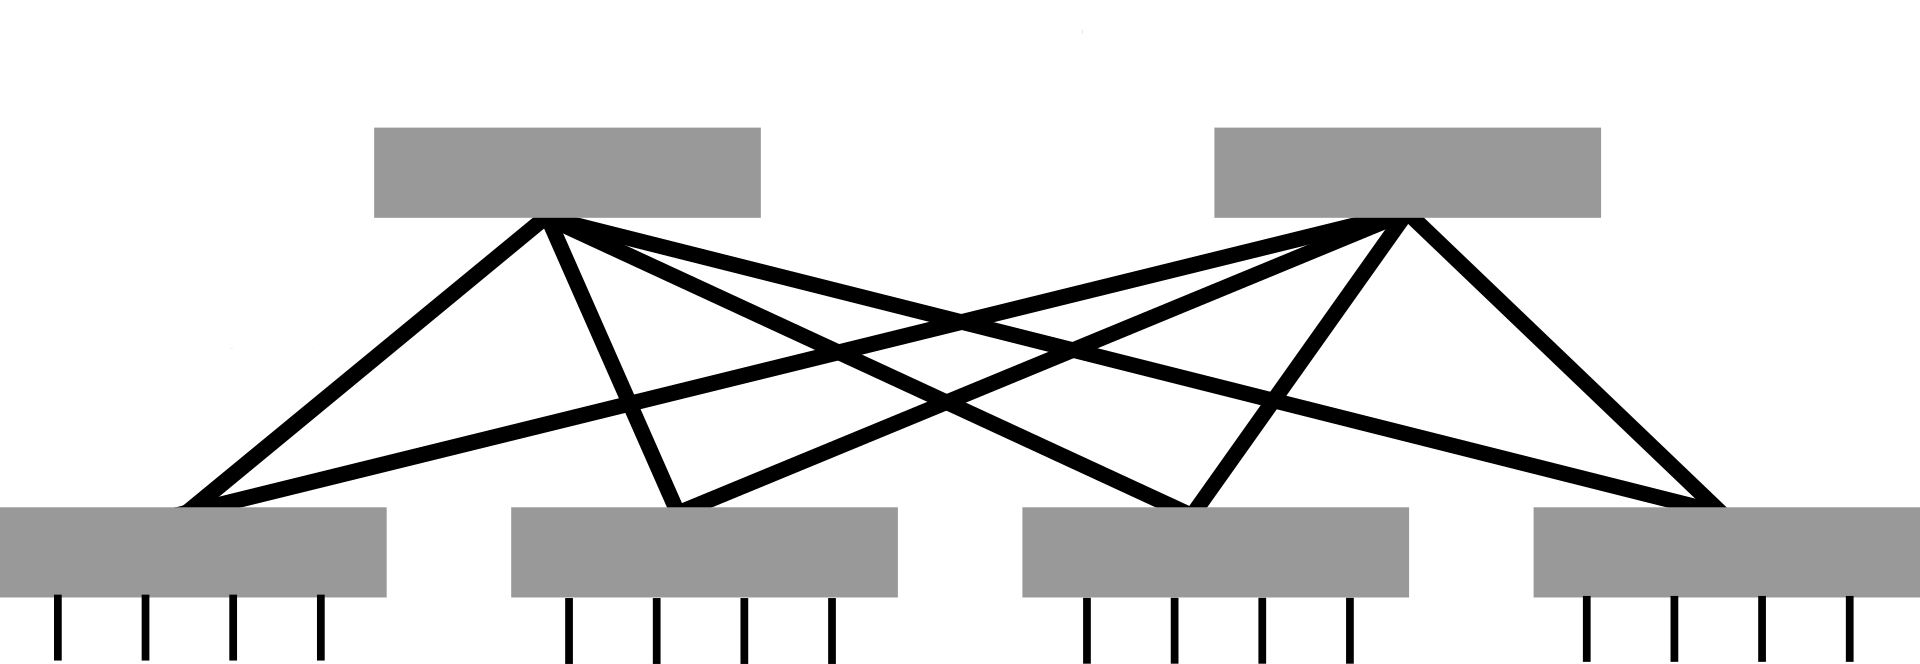
\includegraphics[width = 4.5in]{3_Chapters/2_Chapter_Background/Figs/FatTree.png}
	\caption[Sample fat tree network]{
     Sample fat tree network.
     There are 16 nodes, connected to 4 leaf switches, connected to 2 spine switches acting as the root.
     The thickness of each link represents its bandwidth.
     }
	\label{fig:fat-tree-topology}
\end{figure}


The network topology describes how the nodes are connected, it is often modelled as a graph where vertices are either nodes or switches, and edges represent the network links connecting resources.
In the past, large systems would deploy switchless fabrics, with popular topologies including mesh and torus networks.
Some production clusters still use switchless networks as they map well to the communication patterns of certain HPC applications, but modern commodity hardware has converged on switched topologies, as they are easier to deploy, scale, and manage. 
There are many switched topologies used in practice and proposed in the literature, popular ones include Clos and dragonfly, but the most common switched topology deployed in HPC clusters is fat-tree.
A sample fat tree topology with 16 nodes and two levels is demonstrated in Figure \ref{fig:fat-tree-topology}, similar to a tree data structure, there is a spine switch (the root of the tree) connected to leaf switches (children of the root) which connect to the nodes (leaves of the tree).
Fat-tree get their name because links at the top of the tree will have more bandwidth than links at the bottom, this is because all nodes can potentially send data across the root at the same time.
To save costs, fat trees can be designed with a blocking factor which describes the ratio of available bandwidth at the root compared to the number of children attached to a leaf node, so a non-blocking fat-tree can afford to have all nodes send data across the root at the same time, while a tree with a 5:1 blocking ratio will grind down to 1/5 of the potential bandwidth if all processes go through the spine at the same time.

In HPC communities, the most widely adopted type of network is InfiniBand. 
Similar to PCIe, InfiniBand is a networking standard published by the \textit{InfiniBand Trade Association} (IBTA).
The first InfiniBand spec was published in 2001 with hardware that could support speeds around two Gb/s, but over time the standard and technology have evolved, and now modern InfiniBand networks can transfer data at 400 Gb/s.
The other key characteristic of an HPC network is tremendously low latency, network designers have poured countless hours into removing any possible overhead from the communication code path, some of these key technologies include kernel bypass, hardware tag matching, and network offload.
The InfiniBand specification outlines both the physical characteristics of the network hardware, as well as the InfiniBand verbs programming interface \cite{IBSpec}.
InfiniBand is not the only programming interface, though, and many players have moved in and out of the HPC networking market.
Cornelis Networks develops OmniPath, and Cray has their own line of SlingShot networks, all of which share similar performance and foundational ideas in their design but differ enough to fall across a diverse price/performance spectrum.

\section{Communication libraries} 

There are limits to how applications can interact with the network.
Modern networks have message latencies on the order of microseconds, but with L1 cache latency being on the order of nanoseconds, network transfers are excruciatingly slow.
With drastic performance limits that need to be designed around and a diverse set of network hardware to choose from, a unique set of programming tools are needed to expose network resources. 
There are vast differences in vendor technology as well, different networks have different software layers built on top of them, and portability between networks is an important requirement for many applications. 
So over time, a series of APIs have formed, each targeting different types of users, exposing more/less granularity of the hardware and different types of convenience functions designed to help write code for each layer.
The lowest layer would be device-specific libraries, these are vendor-specific data structures and functions designed to interact directly with hardware on the network card.
Above the device layer would be the transport layer, these are APIs that are designed to lightly wrap around different communication endpoints, they are still not that user-friendly, but they provide more portability and can more easily manage different sets of resources.
The transport layer is used to build programming models, the best example of which is MPI, this is the layer application developers are expected to interact with, it provides the most flexibility and portability for scientific codes.

\subsection{Device APIs and the Transport Layer}

The lowest possible layer of network software are device-specific interfaces, and each vendor has their own; for example, InfiniBand has verbs, Cray's Aries interconnect has GNI, and Intel/Cornellis Netwoks' OmniPath has PSM2 \cite{IBSpec,LibfabricGNICauseCrayisabut,IntelPSM2ProgGuide}.
These APIs are often tightly coupled to device drivers and directly manage memory and registers directly on the network card.
There are often two types of data transfer models, two-sided communication and one-sided communication.
The two-sided model can be thought of as point-to-point messages, applications post send messages indicating which buffers to move to across the network, and the remote peer posts a receive buffer indicating where to place the data.
This model heavily corresponds to MPI send/recv, and network cards often have hardware built in specifically to handle parts of this API.  
The one-sided model, often referred to as Remote Direct Memory Access (RDMA), cuts out the involvement of the remote process.
The remote peer registers a memory region, and the communicating processes can put/get data in that region without remote CPU involvement.
Network cards will also provide atomic memory operations like compare-and-swap and fetch-and-increment, these endpoints perform their function in remote memory without being interrupted by other processes.
These one-sided functions loosely map to MPI's \textit{Remote Memory Access} API, as well as other one-sided programming models like UPC and SHMEM.

Device APIs are the most performant layer, as they are as close as possible to the hardware, but they are often difficult to use and not portable at all.
This is where the transport layer comes in, with the two most well-known interfaces being libfabric and \textit{Unified Communication X} (UCX).
Transport layer libraries provide a programming model that can be easily mapped to multiple types of hardware but still be abstract and portable enough so that vendors can add/remove features specific to their hardware.
When instantiating a libfabric endpoint, users explicitly chose the type of network they want to establish, and options can include specific vendors, TCP sockets, shared memory, and many more.
So libfabric provides an abstraction of the network resources, some registration routines, and a work queue-based communication model for one-sided and two-sided communications \cite{libfabric}.
In the work queue model, processes post communication requests on a work queue and poll a corresponding completion queue for communication completion, the benefit of this model is that it maps very closely to how the hardware works.
One catch with libfabric is that higher-level programming models still have to manage multiple types of resources to ensure that the proper hardware is used for the appropriate transactions. 
However, UCX avoids this problem by handling transport selection.
UCX provides similar abstractions for network resources, memory registration and one/two-sided communication, but the communication model is based on callbacks to notify completion \cite{shamis2015ucx}.
This callback-based model provides more flexibility to user implementation at the cost of increased overhead.
While their completion models differ, both support point-to-point messages (tagged and untagged) and one-sided operations, and both communication models are frequently used by higher-level libraries or have hardware optimizations built into high-performance network cards.
Both libraries also support (or at least specify support for) accelerators, this means it is possible to pass device buffers into communication operations and expose device memory for RDMA.

These interfaces are a lot friendlier and provide nicer and more portable endpoints than vendor APIs, but they still have a lot of rough edges, and the target audience is systems developers, not domain scientists.
Transport layer libraries often expect users to perform a lot of memory and device management, which can place a lot of unnecessary burdens on application developers.
That's why there is one more layer above the transport layer, the programming model layer, which is intended to be used by a more science-focused audience.

\subsection{MPI}
At the highest level, application developers are expected to use a programming model to build their scientific apps. 
While there are multiple types of distributed memory programming models, MPI is by far the most prevalent and widely used.
The MPI-forum, the academic/industry body that is responsible for standardizing MPI, is often the bridge between the application community and the networking community.
The first MPI specification was released in 1994 and started as a two-sided programming model with support for collective communications, and has evolved over time with MPI-2, published in 1997, adding support for a one-sided programming model, and the latest spec, MPI-4, specifying many more features like neighbourhood collectives, partitioned communication, virtual topologies, datatype management, distributed I/O and more.

MPI is a programming model for multi-process distributed memory programming, so at program launch, each process needs to be created by a call to \texttt{fork()}, and connection information (including but not limited to hostname and PID) needs to be distributed among all processes. 
Process creation is handled by \texttt{mpiexec}, a program MPI implementations must provide, and users can specify how many processes to launch, how to bind processes to resources and the location of the executable file.
Inside the user's code, the first MPI routine that can be called is \texttt{MPI\_Init()}, which is responsible for instantiating the MPI library, and performs tasks like network card initialization and wireup.
One of the data structures \texttt{MPI\_Init()} sets up is the global communicator \texttt{MPI\_COMM\_WORLD}, communicators are a structure encapsulating a set of processes that can exchange data with each other, and \texttt{MPI\_COMM\_WORLD} contains every process launched by \texttt{mpiexec}.
Each process in a communicator is assigned a rank, a unique identifier ranging from zero to the size of the communicator minus 1, and these ranks are used to identify an individual process within a communicator.
\texttt{MPI\_Init()} instantiates the global communicator, but applications can create new communicators, this can be used to carve out smaller groups of processes or renumber processes to map to a topological structure.

In order to comprehend why MPI is so powerful, it is necessary to understand MPI's message-passing model, this interface specifies how two processes exchange data.
Point-to-point messages can be extended to a collective model where multiple processes exchange data in a pre-determined manner, these communication routines are extremely powerful and heavily relied upon. 
Further, the one-sided model is also important, as it provides a set of tools for managing communication without peer involvement.

\subsubsection{Two-Sided Communications}

The two-sided model is built around sending and receiving messages across a communicator.
Messages are specified as a vector of MPI datatypes, which can vary from a simple array of integers to complex structures of derived datatypes that require special handling to pack into buffers. 
\texttt{MPI\_Send()} specifies a segment of data to send to a remote process, and the remote process must post a corresponding \texttt{MPI\_Recv()} indicating where the data will be placed. 
The send operation identifies the destination through a tuple containing a rank, tag, and communicator, the corresponding receive must match these fields or contain wildcard values for \texttt{MPI\_ANY\_SOURCE} or \texttt{MPI\_ANY\_TAG}.

There are a few nuances and gotchas to the message-passing model.
Messages are non-overlapping, so if two back-to-back sends can match the same receive operation, then the first message needs to complete before the second, and standard MPI operations are blocking, this means program execution halts at the communication call until the operation is complete.
If the programmer is not careful, this can lead to deadlocks, for example, a process can get stuck in a blocking receive that doesn't have a corresponding send, and the program will hand.

In a later version of the MPI specification, non-blocking messages were introduced with corresponding \texttt{MPI\_Isend()}/\texttt{MPI\_Irecv()} functions.
These endpoints return immediately but don't complete communication, instead, they populate an \texttt{MPI\_Request} object with information about the ongoing communication.
The programmer needs to progress the \texttt{MPI\_Request} object in order to ensure completion, this can be done with \texttt{MPI\_Test} to check if it's done and \texttt{MPI\_Wait} to block communication until completion.
Non-blocking communications provide more flexibility and freedom in setting up complex communication patterns, as well as more opportunities to establish computation communication overlap.

\subsubsection{One-sided Communication}
The term two-sided exists because both processes have to actively be involved in communication (a send needs a matching receive), the model is popular because it is easy to understand and learn quickly but is limited by the tightly coupled nature of the communication model.
Certain applications do not map well to the two-side model, there are codes where processes need to send/receive data between iterations but don't necessarily know who they will need to exchange with, and while solutions can be coded using a one-sided model, it requires the use of heavy global synchronizations heavily impacting performance, 
The one-sided model, also known as Remote Memory Access (RMA), provides a model where only one process needs to provide the communication information, message data, message destination, and participating ranks.
One-sided operations are performed on a window, an opaque object encapsulating network-exposed memory on a communicator, the target rank is the process that owns memory in the window, and the origin process is the remote rank accessing the target's data.
Load/store operations are triggered on a window using \texttt{MPI\_Get()}/\texttt{MPI\_Put()} functions, and remote arithmatic can be done using \texttt{MPI\_Accumulate()} or \texttt{MPI\_Fetch\_and\_op()}.
Many of the data parameters for one-sided can be mapped to values in the sided model, a rank is specified, and operations accept buffers of MPI\_Datatypes for the origin's local data and the target's data within the window.

The challenge with RMAs is synchronization, shared memory type models are prone to data races, and the MPI standard tries to establish a series of guard rails to make writing applications much easier.
By default, all MPI RMA operations are non-blocking, calling \texttt{MPI\_Get()}/\texttt{MPI\_Put()} triggers a communication operation but does not guarantee completion.
MPI RMA operations have multiple mechanisms to choose from for enforcing ordering and completion.
The most straightforward synchronization method is to use \texttt{MPI\_Win\_Fence()}, this operation acts as a collective barrier across a window, and all processes must call \texttt{MPI\_Win\_Fence()} before proceeding, but it guarantees that all outstanding one-sided operations are completed on a window before proceeding. 
There is an active communication model which relies on four endpoints (\texttt{MPI\_Win\_start}, \texttt{MPI\_Win\_complete}, \texttt{MPI\_Win\_post}, and \texttt{MPI\_Win\_wait}) and provides a mechanism for the target process to dictate when remote processes can access its window.
The target starts an access epoch with \texttt{MPI\_Win\_start}, next the origin rank must call \texttt{MPI\_Win\_post} to synchronize with the remote peer and gain exclusive access to the window, now the target can issue put/get/accumulate calls as necessary.
To finish communication, the origin calls \texttt{MPI\_Win\_wait}, this cleans up all outstanding communication requests, now another rank can try and gain access through their own call to \texttt{MPI\_Win\_post}, or the target can close the window by calling \texttt{MPI\_Win\_complete}.
The last mechanism is \texttt{MPI\_Win\_lock}/\texttt{MPI\_Win\_unlock}, these primitives are essentially mutexes, they let ranks establish shared or exclusive access to a window, and all outstanding operations are guaranteed completion on MPI\_Win\_unlock().


\subsubsection{Collective Communication}

\begin{figure}
	\centering
	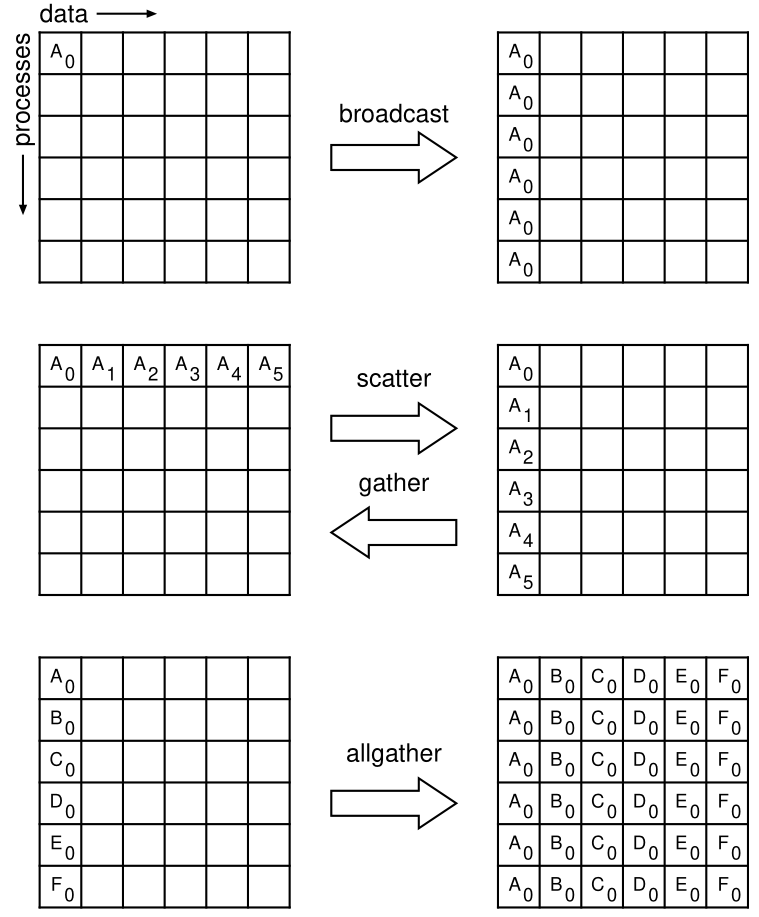
\includegraphics[width = 4.5in]{3_Chapters/2_Chapter_Background/Figs/mpispec_collective.png}
	\caption[Demonstration of collective communications]{
     Demonstration of collective communications taken from \cite{mpi40}.
     Columns specify each process' rank, and rows specify elements in the input vector.
     }
	\label{fig:mpispec_collectives}
\end{figure}

MPI's point-to-point and RMA models specify data transfers between two processes, but often when writing MPI codes, several common patterns arise which require data exchanges among multiple processes at the same time.
These patterns are known as collective communications, and they are common enough that the MPI-forum has standardized several of them.
A few example collectives are outlined in figure \ref{fig:mpispec_collectives}, collectives take a data buffer and transfer the data buffer across all ranks in a communicator.
Collectives can be generalized into two groups, \textit{all-to-one} and \textit{all-to-all} collectives.
All-to-one collectives have a specified root that can act as the main source/destination for all data, for example, \texttt{MPI\_Bcast()} distributes a chunk of data specified by the root to all processes in the communicator.
All-to-all collectives have every process both contribute and receive some set of data within the operations, with, for example, in \texttt{MPI\_Allgather()} each process specifies a segment of data and all the segments are combined into a larger vector (indexed by rank) with a copy of the final result distributed to each process.

The reduction collectives, \texttt{MPI\_Reduce()} and \texttt{MPI\_Allreduce()}, are collectives of particular interest as they are heavily relied upon and can take up large parts of overall application run time.
Their defining characteristic is that accepts an operation which is applied to the data in flight.
\texttt{MPI\_Reduce()} is an all-to-one collective where each process specified a buffer and result is placed at the root, while \texttt{MPI\_Allreduce()} is an all-to-all style collective where each process receives a copy of the final result. 
As an example, if each process had a double and the average across all doubles was necessary for the next step of the computation, each process could call \texttt{MPI\_Allreduce()} with a type \texttt{MPI\_DOUBLE} with the op \texttt{MPI\_SUM} to get the sum of each rank's double, and then divide the result by the communicator size to get the average.

Collective communications are considerably powerful as they can express a lot of data movement in a single operation, and for this reason, they are heavily used in production codes.
But, the inherent downside of collectives is the amount of synchronization they can apply to parallel programs. 
Collectives can be blocking operations, and they require all processes in a communicator to participate in the operation, so they often have the side effect of stalling the entire program waiting for processes to arrive.
Non-blocking collectives do exist, like the point-to-point interface, they return an \texttt{MPI\_Request} object that needs to be progressed with \texttt{MPI\_Test}/\texttt{MPI\_Wait}, but adoption isn't that large and many codes still rely on blocking operations.
The popularity, yet simultaneous optimization challenges, have led to a large body of research on the topic of collective communication. 
There are plethora of strategies for designing collective algorithms, two of which we rely on for this thesis including topology-awareness and process arrival pattern awareness.

\subsubsection{Algorithm Structure}
Under the hood, collective algorithms are implemented as a series of point to point messages. 
There are different ways to structure the exchanges in order to implement a specified collective, and different structures have different performance tradeoffs depending on the collective's parameters.
One of the most impactful parameters in communication is the size of the message, and it is best examplified through Hockney's model \cite{Hockney1994HockenyModel}.
Hockney's model states that the time to send a message of $n$ bytes can be modeled as $T_{msg}=\alpha+n\beta$, where $\alpha$ represents the startup overhead cost (seconds) and $\beta$ is inverse bandwidth (seconds per byte).
What tends to happen in practice is that small messages are bound by $\alpha$, while large messages spend most of their time bandwith bound by $n\beta$.
This principle extends this to collective algorithms, where designes tend to fall into the same two categories, latency bound for small messages and bandwidth bound for large messages.
Latency bound algorithms try to minimize the number of messages sent as the fewer times we invoke $\alpha$ the faster the algorithm, while large message algorithms will break the data vector into components and issue multiple smaller message minimizing the total amount of data sent.
When dealing with reduction operations, we can add a $\gamma$ term which represents the time to perform a reduction in seconds per flop, similar to the $\beta$ term this scales by $n$.

\begin{figure}
    \centering
    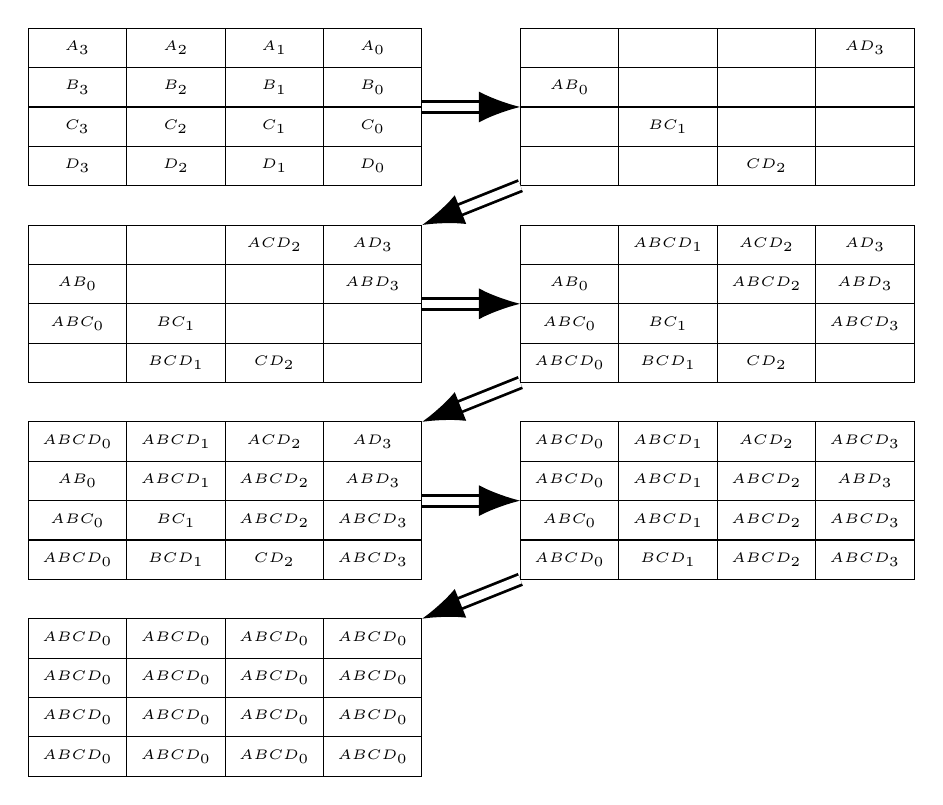
\begin{tikzpicture}[auto]
    
        \def \bkxscale {1.25}
        \def \bkyscale {0.5}
        \begin{scope}[every node/.style={draw, rectangle}, minimum height=0.5cm, minimum width=1.25cm, font=\tiny]
            \foreach \y in {0,1,2,3} \foreach \x in {0,1,2,3} \node at (\x*\bkxscale,\y*\bkyscale) (a\x\y) {$ABCD_{0}$};
            \foreach \y in {10,11,12,13} \foreach \x in {0,1,2,3} \node at (\x*\bkxscale,\y*\bkyscale) (d\x\y) {};
            \foreach \y in {10,11,12,13} \foreach \x in {5,6,7,8} \node at (\x*\bkxscale,\y*\bkyscale) (e\x\y) {};
            \foreach \y\ly in {15/D,16/C,17/B,18/A} \foreach \x\lx in {0cm / 3,1cm / 2,2cm / 1,3cm / 0} \node at (\x*\bkxscale,\y*\bkyscale) (f\x\y) {$\ly_{\lx}$};
            \foreach \y in {15,16,17,18} \foreach \x in {5,6,7,8} \node at (\x*\bkxscale,\y*\bkyscale) (g\x\y) {};
        
            \draw[line width=1pt, double distance=3pt, arrows = {-Latex[length=0pt 3 0]}] (3.5*\bkxscale, 16.5*\bkyscale) -- (4.5*\bkxscale, 16.5*\bkyscale);
            \draw[line width=1pt, double distance=3pt, arrows = {-Latex[length=0pt 3 0]}] (3.5*\bkxscale, 11.5*\bkyscale) -- (4.5*\bkxscale, 11.5*\bkyscale);
            \draw[line width=1pt, double distance=3pt, arrows = {-Latex[length=0pt 3 0]}] (3.5*\bkxscale, 6.5*\bkyscale) -- (4.5*\bkxscale, 6.5*\bkyscale);
            \draw[line width=1pt, double distance=3pt, arrows = {-Latex[length=0pt 3 0]}] (4.5*\bkxscale, 14.5*\bkyscale) -- (3.5*\bkxscale, 13.5*\bkyscale);
            \draw[line width=1pt, double distance=3pt, arrows = {-Latex[length=0pt 3 0]}] (4.5*\bkxscale, 9.5*\bkyscale) -- (3.5*\bkxscale, 8.5*\bkyscale);
            \draw[line width=1pt, double distance=3pt, arrows = {-Latex[length=0pt 3 0]}] (4.5*\bkxscale, 4.5*\bkyscale) -- (3.5*\bkxscale, 3.5*\bkyscale);
            
            \node at (5*\bkxscale, 17*\bkyscale) (comebacktome) {$AB_0$};
            \node at (6*\bkxscale, 16*\bkyscale) (comebacktome) {$BC_1$};
            \node at (7*\bkxscale, 15*\bkyscale) (comebacktome) {$CD_2$};
            \node at (8*\bkxscale, 18*\bkyscale) (comebacktome) {$AD_3$};
            
            \node at (0*\bkxscale, 12*\bkyscale) (comebacktome) {$AB_0$};
            \node at (1*\bkxscale, 11*\bkyscale) (comebacktome) {$BC_1$};
            \node at (2*\bkxscale, 10*\bkyscale) (comebacktome) {$CD_2$};
            \node at (3*\bkxscale, 13*\bkyscale) (comebacktome) {$AD_3$};
            \node at (0*\bkxscale, 11*\bkyscale) (comebacktome) {$ABC_0$};
            \node at (1*\bkxscale, 10*\bkyscale) (comebacktome) {$BCD_1$};
            \node at (2*\bkxscale, 13*\bkyscale) (comebacktome) {$ACD_2$};
            \node at (3*\bkxscale, 12*\bkyscale) (comebacktome) {$ABD_3$};
            
            \node at (5*\bkxscale, 12*\bkyscale) (comebacktome) {$AB_0$};
            \node at (6*\bkxscale, 11*\bkyscale) (comebacktome) {$BC_1$};
            \node at (7*\bkxscale, 10*\bkyscale) (comebacktome) {$CD_2$};
            \node at (8*\bkxscale, 13*\bkyscale) (comebacktome) {$AD_3$};
            \node at (5*\bkxscale, 11*\bkyscale) (comebacktome) {$ABC_0$};
            \node at (6*\bkxscale, 10*\bkyscale) (comebacktome) {$BCD_1$};
            \node at (7*\bkxscale, 13*\bkyscale) (comebacktome) {$ACD_2$};
            \node at (8*\bkxscale, 12*\bkyscale) (comebacktome) {$ABD_3$};
            \node at (5*\bkxscale, 10*\bkyscale) (comebacktome) {$ABCD_0$};
            \node at (6*\bkxscale, 13*\bkyscale) (comebacktome) {$ABCD_1$};
            \node at (7*\bkxscale, 12*\bkyscale) (comebacktome) {$ABCD_2$};
            \node at (8*\bkxscale, 11*\bkyscale) (comebacktome) {$ABCD_3$};
            
            \node at (0*\bkxscale, 7*\bkyscale) (comebacktome) {$AB_0$};
            \node at (1*\bkxscale, 6*\bkyscale) (comebacktome) {$BC_1$};
            \node at (2*\bkxscale, 5*\bkyscale) (comebacktome) {$CD_2$};
            \node at (3*\bkxscale, 8*\bkyscale) (comebacktome) {$AD_3$};
            \node at (0*\bkxscale, 6*\bkyscale) (comebacktome) {$ABC_0$};
            \node at (1*\bkxscale, 5*\bkyscale) (comebacktome) {$BCD_1$};
            \node at (2*\bkxscale, 8*\bkyscale) (comebacktome) {$ACD_2$};
            \node at (3*\bkxscale, 7*\bkyscale) (comebacktome) {$ABD_3$};
            \node at (0*\bkxscale, 5*\bkyscale) (comebacktome) {$ABCD_0$};
            \node at (1*\bkxscale, 8*\bkyscale) (comebacktome) {$ABCD_1$};
            \node at (2*\bkxscale, 7*\bkyscale) (comebacktome) {$ABCD_2$};
            \node at (3*\bkxscale, 6*\bkyscale) (comebacktome) {$ABCD_3$};
            \node at (0*\bkxscale, 8*\bkyscale) (comebacktome) {$ABCD_0$};
            \node at (1*\bkxscale, 7*\bkyscale) (comebacktome) {$ABCD_1$};
            \node at (2*\bkxscale, 6*\bkyscale) (comebacktome) {$ABCD_2$};
            \node at (3*\bkxscale, 5*\bkyscale) (comebacktome) {$ABCD_3$};
            
            \node at (5*\bkxscale, 7*\bkyscale) (comebacktome) {$ABCD_0$};
            \node at (6*\bkxscale, 6*\bkyscale) (comebacktome) {$ABCD_1$};
            \node at (7*\bkxscale, 5*\bkyscale) (comebacktome) {$ABCD_2$};
            \node at (8*\bkxscale, 8*\bkyscale) (comebacktome) {$ABCD_3$};
            \node at (5*\bkxscale, 6*\bkyscale) (comebacktome) {$ABC_0$};
            \node at (6*\bkxscale, 5*\bkyscale) (comebacktome) {$BCD_1$};
            \node at (7*\bkxscale, 8*\bkyscale) (comebacktome) {$ACD_2$};
            \node at (8*\bkxscale, 7*\bkyscale) (comebacktome) {$ABD_3$};
            \node at (5*\bkxscale, 5*\bkyscale) (comebacktome) {$ABCD_0$};
            \node at (6*\bkxscale, 8*\bkyscale) (comebacktome) {$ABCD_1$};
            \node at (7*\bkxscale, 7*\bkyscale) (comebacktome) {$ABCD_2$};
            \node at (8*\bkxscale, 6*\bkyscale) (comebacktome) {$ABCD_3$};
            \node at (5*\bkxscale, 8*\bkyscale) (comebacktome) {$ABCD_0$};
            \node at (6*\bkxscale, 7*\bkyscale) (comebacktome) {$ABCD_1$};
            \node at (7*\bkxscale, 6*\bkyscale) (comebacktome) {$ABCD_2$};
            \node at (8*\bkxscale, 5*\bkyscale) (comebacktome) {$ABCD_3$};
            
        \end{scope}
        
    \end{tikzpicture}
    \caption{
        Ring allreduce algorithm. Each grid represents a step in the algorithm, where rows are ranks and columns are segments of the data vector.
    }
    \label{fig:ring-allreduce-grid} 
\end{figure}
Figure \ref{fig:ring-allreduce-grid} outlines a four rank ring allreduce.
The ring algorithm is oftenly used for large message allreduce because bandwitdh based performance scales linearly.
During each step of the algorithm, each rank $r$ sends a message to rank $r+1$ and recieves a message from rank $r-1$, this is where the ring algorithm gets its name from.
For a ring of $p$ processes, the first $p-1$ steps consist of a data exchange and reduction operation, where each chunk of data conssists of $n/p$ Bytes of data. 
At the midway point, each rank will hold $1/n$ of the fully reduced vector, this data distribution can be considered as a reduce-scatter.
The algorithm finishes with another $p-1$ messages of size $n/p$, this time without the reduce, which act as an allgather distributing the final result.
In total, $2(p-1)$ messages of size $n/p$ are sent, with half of them requireing a reduction, this can give us a total collective time of $T_{ring} = 2(p-1)\alpha + 2((p-1)/p)n\beta + ((p-1)/p)n\gamma$.
The ring algorithm can be generalized to a reduce-scatter folowed by an allgather, and it is possible to implement both in a recussive-doubling method, this is also known as Rabenseifner's algorithm \cite{Thakur2005OptMPICH}.
This change can lower the number of data exchanges to $2\log(p)$, but will require an extra communication stage to ballance data if $p$ is not a power of 2.

One-to-all type collective algorithms can often modelled as trees where vertices are ranks, edges between verticeis are messages, and the root of the tree is the root of the collective.
The stucture of the tree will have an imact on collective time, for example, a binary would theorheticly perform better than a linear tree (also known as a chain) due to the logarithmic nature of its height.
Collective algorithms can also leverage message pipelineing techniques, where a message is broken into segments and be propogated through a tree letting different segments overlap each other.
By default, a chain broadcast would take $T_{chain}=p\alpha+pn\beta$, but with a segment size of $k$ it could be performed in $T_{chain\_pipe}=(n/k+p-1)\alpha+(n+(p-2)k)\beta$.
Pipelining leverages concurrency by sending multiple stages in parallel and shows the most benifit from a bandwith perspective.

\subsubsection{Topology Awareness}
The desing of the machine is important
Adding topology awareness, 
Hierarchical algs
\subsubsection{Process Arrival Pattern Awareness}
Not all procs arrive at the same time
\subsubsection{Algorithm selection}
Different algs are better in different scenarios


% Chapter 3 - Methodology

% \glsresetall % reset the glossary to expand acronyms again
\chapter[Large Scale Distributed Deep Learning]{Large Scale Distributed Deep Learning}\label{ch:CH3-DistributedDL}
\index{Distributed Deep Learning}
Over the past decade, \gls{ML}, specifically \gls{DL}, has exploded in popularity.
Several incredibly challenging problems have recently been solved using emerging techniques, classic examples include computer vision \cite{Krizhevsky2012AlexNet}, and natural language processing \cite{Vaswani2017AttentionTransformer}.
Furthermore, more traditional scientific \gls{HPC} fields like climate modelling \cite{Ham2019DLENSOForcasts} and cosmology \cite{Mathuriya2019Cosmoflow} are starting to adopt \gls{DL} methods.
There is an incredible demand for \gls{DL} as academia and industry rush to develop new models to solve more problems.
However, \gls{DL} is incredibly computationally intensive, and depending on the number of model parameters and the dataset size, training time can span from hours to weeks.
To address these issues, \gls{DL} practitioners are adopting \gls{HPC} techniques to parallelize the training process at a massive scale and build larger models faster.
Parallelization strategies are diverse, but the three methods used at scale are hyperparameter search for evaluating different architectures, model parallelism to stretch a model across multiple nodes, and data parallelism to process numerous samples concurrently and lower time to convergence.
Data parallelism is the most well-understood parallelization strategy, having existed long before the recent AI revolution \cite{Zhang1990BPonCM2}.
It is relatively easy to deploy, has a well-understood communication pattern, and is highly scalable.

This chapter contains a high-level overview of current distributed \gls{DL} practices focusing on data-parallel strategies.
We then outline the state-of-the-art tools used at scale and investigate \gls{HPC} methods that have accelerated data-parallel training in literature.

\section{Deep Learning}
DL is a supervised learning technique where a model is trained to approximate some ground truth source, typically a dataset.
Formally, \gls{DL} training tries to find a function $f: X\longrightarrow Y$ which maps data from sample space $X$ to label space $Y$.
To predict how accurate $f$ is for a sample $x$, we define a loss function \\ $L_D(f)=\mathbb{P}[f(x)\neq h(x)]$, where $x$ is a sample in dataset $D$ with label $h(x)$.
In practice, $f$ will belong to a class of function $\mathcal{H}$ containing functions $f_w$, where $w$ is a vector of parameters.
To train a model, a training algorithm will try to find some value for $w$ which minimizes the loss function of $f$ over $D$, formally:
\begin{equation}
    \argmin_{w\in\mathcal{H}} L_D(f_w) = \argmin_{w\in\mathcal{H}} \mathbb{E}_{x\in D}[\ell (w,x)]
    \label{eq:argmin-loss}
\end{equation} 
where $\ell:\mathcal{H}\times X\longrightarrow \mathbb{R}^+$ is the loss function for an individual sample. 

Many optimization algorithms can solve Equation \ref{eq:argmin-loss}, but the most widely adopted algorithm is \gls{SGD}.
Standard gradient descent relies on a continuous optimization space to intelligently sample points, but the datasets used in \gls{DL} are not continuous.
SGD methods used in practice randomly sample points in the dataset, and while they do converge, they tend to take much longer than traditional gradient descent \cite{Robbins1951StochasticAproxmethod}.
Traditional \gls{SGD} samples one data point at a time, but on modern hardware, we can increase device utilization, and throughput by grouping multiple data points using a batch method \cite{Le2011OnOptMethodsforDL}.
Batch methods sample a set of data points to assemble a batch, calculate an update step for each sample in the batch, and apply the average update of the batch to the model. 

\begin{algorithm}[h]
    \DontPrintSemicolon
    \For {t = 0 \textbf{to} $\frac{|D|}{B}*epochs$} {
        $\Bar{x}\leftarrow$ Vector of $B$ Random elements from $D$ \;
        $w_{mb}\leftarrow w^{(t)}$ \;
        $f\leftarrow \ell(w_{mb},\Bar{x},h(\Bar{x}))$ \;
        $g_{mb}\leftarrow \nabla \ell(w_{mb}, f)$ \;
        $\Delta w \leftarrow u(g_{mb}, w^{(0,...,t)}, t)$ \;
        $w^{(t+1)}\leftarrow w_{mb} + \Delta w$ \;
    }
    \caption{Minibatch SGD}
    \label{alg:MinibatchSGD}
\end{algorithm}

Algorithm \ref{alg:MinibatchSGD} provides a textbook example of a minibatch \gls{SGD} algorithm.
The main loop of the algorithm iterates over the entire dataset in what is known as an epoch, often done a predefined number of times. 
Still, other stopping criteria can include an evaluation threshold on an external validation dataset or a collapse in the loss function.
A batch of data is sampled from the training dataset in Line 2, the dataset is shuffled between epochs to generate different minibatches for each epoch.
The minibatch samples are propagated through the model in the forward pass on Line 4, and the set of forward pass results is used to calculate a set of gradients in Line 5. 
Line 6 uses an update function to calculate the weight updates.
This function is responsible for combining the gradients of all the samples into weight updates to be applied to the next iteration of the model (Line 7).

While this algorithm seems straightforward, the research space is massive, spanning from the model's architecture to tweaking parts of the training algorithm.
The optimization space can have multiple minimums, and deliberate steps must be taken to ensure the global minimum is found. 
Weight initialization is another issue since the final accuracy can be heavily influenced by $w^{(0)}$.
There is a wide body of research proposing different initialization methods, and popular techniques involve random values, informed decisions, or transfer learning from other pre-trained models \cite{Glorot2010XavierInitalization}.
The weight update rule $u$ has also undergone a lot of research.
If update steps are too large, the model will not generalize and will be unstable, but if updates are too small, training can take an exceedingly long time and fail to converge.
The most straightforward rule, $u_{sgd}(g)=-\eta \cdot g$, multiplies the gradient by a learning rate $\eta$, but the learning rate can be changed over time, with a common practice of exponentially shrinking the gradient with larger values of $t$.
More clever methods can include momentum, which uses the difference between current and past weights to influence update magnitude, and modern techniques, like Adam \cite{Kingma2015Adam}, leverage the first and second moments of the gradient to update learning rates individually for each weight in the model.

The model's architecture also plays an important role.
The founding idea for neural networks was to approximate the structure of neurons in the brain mathematically.
Individual neurons take a set of inputs, calculate a weighted sum across a set of weights, apply an activation function to introduce nonlinearity, and pass the output on to other neurons. 
Neurons are organized into layers, often structured in a fully connected manner where the output of one neuron is connected to every neuron in the next layer.
The model's width is defined by the number of neurons in a layer, while the number of layers defines the depth.
These early feed-forward networks have a powerful ability to learn non-linear relationships and can be efficiently implemented using \gls{GEMM}.
However, different layer types have been proposed which can extract specific features of different kinds of data; famous examples include convolutional layers for images \cite{Krizhevsky2012AlexNet}, recurrent layers for sequence data \cite{cho2014PhraseRepresentationRNN}, and transformer layers for text \cite{Vaswani2017AttentionTransformer}.
Further, many different activation functions can be used, with popular choices including sigmoid and rectified linear units \cite{Nair2010ReLU}.

However, one prevalent trend of \gls{DL} (in fact, this is where the 'deep' in \textit{deep learning} comes from) is that larger models and larger datasets give better performance \cite{Kaplan2020ScalingLawsForNLModels, Ben-Nun2019DemystifyDL}.
There is a consistent trend of larger models training on larger datasets; however, the more these factors increase in scale, the required training time scales in tandem.
To address these issues, several parallelization strategies have been applied.

Individual layer operations were the initial target for optimization. 
Many hardware providers have released software libraries designed to run layer-specific operations like convolutions and \gls{GEMM} as fast as possible; examples include Intel's MKL \cite{MKL} and Nvidia's cuDNN \cite{cuDNN}. 
The compute-intensive nature of \gls{DL} models has led to the wide adoption of \gls{GPU}s as the massively parallel capabilities of these accelerators can blast through training and inference orders of magnitude faster than \gls{CPU}s.
\gls{GPU}s still have a limit to how many T\gls{FLOPS} they can drive, and there are limits to the amount of accelerator memory, but both limitations can be broken by scaling across a cluster.

\section{Deep Learning Parallelization Strategies}
Mapping \gls{DL} training to a distributed memory environment creates several unique challenges.
The three most common strategies for parallelizing \gls{DL} are hyperparameter search, where model architectures are evaluated concurrently; model parallelism, where a model's weights are distributed across resources; and data parallelism, which leverages parallelism in the training algorithm to concurrently evaluate samples in a batch.
Each method has its strength and targets a slightly different aspect of \gls{DL} scaling while having its corresponding performance characteristics that must be accounted for.

\subsection{Hyperparameter search}
The features specifying a \gls{DL} model can be lumped into two categories, parameters and hyperparameters.
Parameters are values filled by the optimization algorithm and is essentially synonymous with the model's weights. 
Conversely, hyperparameters focus on specifying the structure of the model and remain unchanged during training.
Hyperparameters include structural features of the model, like the number and types of layers, activation function, and loss function. 
They can also extend to the training algorithm with tunables like learning rate, learning rate decay, and batch size.
The setup has an outsized impact on model performance, so often, a lot of model development time goes into hyperparameter selection. 
However, each new hyperparameter adds another search dimension and exponentially increases the search space.
Therefore, automated hyperparameter search strategies are a popular target for parallelization at scale.

Research in hyperparameter search systems tends to investigate the search algorithm. 
Initially proposed search algorithms include sequential search heuristics, like grid search \cite{Hadjis2016Omnivore}, where a series of candidates are identified, models are trained for each, and the search space is iteratively refined based on the training results.
More clever techniques have used evolutionary algorithms \cite{Young2017EvolveNLWithHPC, Real2017LargeScaleEvolutionOfCV}, which generates a population of candidate models and iteratively removes underperforming models and replaces them with higher-performing models with random perturbations, or reinforcement learning \cite{Zoph2017NeuralArchSearchReinformceLearn} which uses gradient-based optimization to discover more optimal model architectures.

At its core, hyperparameter search trains a \gls{DL} model (which can take tens of minutes to hours), validates the model's performance, and updates a search space (send and receive a few megabytes).
This makes hyperparameter search an incredibly compute-intensive task with little communication, making it a great candidate for parallelization.
Large-scale hyperparameter search systems are often based on a server/worker design, where the centralized server manages the search algorithm and issues models for worker nodes to train and evaluate.
These systems generate relatively little communication as model architectures can be specified in a few bytes, workers can take hours to train a model, and they have been relatively easy to scale to exceedingly large systems \cite{Young2017EvolveNLWithHPC}.

\subsection{Model Parallelism}
\begin{figure}
    \centering
        \begin{tikzpicture}[
        nsty/.style={draw,circle,minimum height=0.5cm},
        psty0/.style={fill=blue!40},
        psty1/.style={fill=yellow!40},
        psty2/.style={fill=red!40},
        imgsty/.style={draw,rectangle,fill=white,
            minimum height=1.5cm,
            minimum width=1.5cm,
        },
        arrowsty/.style={draw, single arrow, rotate=-90,
            fill=white,
            minimum height=0.7cm,
        },
        snsty/.style={draw,circle,minimum height=0.2cm},
        simgsty/.style={draw,rectangle,minimum height=0.5cm,minimum width=0.5cm},
        sarrowsty/.style={draw, single arrow, rotate=-90,
            fill=white,
            minimum height=0.4cm,
            minimum width=0.01cm,
        },
    ]

    \foreach \x in {0,1,2}
        \foreach \y in {0,1,2}
            \node[snsty,psty0] at (\x/2-4.5, \y/2+2) (s\x\y0) {};
    \node[simgsty,psty0] at (-4,4) (si0) {};
    \draw[->] (si0) -- node[midway,right, font=\tiny]{Input} (s120);
    \draw[->] (s100) -- node[midway,right, font=\tiny]{Output} +(0,-0.5);
    \node[left=0.01cm of s020.130] {$p_0$};
            
    \foreach \x in {0,1,2}
        \foreach \y in {0,1,2}
            \node[snsty,psty1] at (\x/2-6, \y/2) (s\x\y1) {};
    \node[simgsty,psty1] at (-5.5,2) (si1) {};
    \draw[->] (si1) -- node[midway,right, font=\tiny]{Input} (s121);
    \draw[->] (s101) -- node[midway,right, font=\tiny]{Output} +(0,-0.5);
    \node[left=0.01cm of s021.130] {$p_1$};
    
            
    \foreach \x in {0,1,2}
        \foreach \y in {0,1,2}
            \node[snsty,psty2] at (\x/2-3, \y/2) (s\x\y2) {};
    \node[simgsty,psty2] at (-2.5,2) (si2) {};
    \draw[->] (si2) -- node[midway,right, font=\tiny]{Input} (s122);
    \draw[->] (s102) -- node[midway,right, font=\tiny]{Output} +(0,-0.5);
    \node[left=0.01cm of s022.130] {$p_2$};

    \foreach \n in {0,1,2}
        \foreach \x in {0,1,2}
            \foreach \y in {0,1,2}{
                \draw[] (s\x0\n) -- (s\y1\n);
                \draw[] (s\x2\n) -- (s\y1\n);
            }


    \foreach \x in {0,1,2}
        \foreach \y in {0,1,2}
            \node[nsty,psty\x] at (\x,\y) (n\x\y) {};
            
    \foreach \x in {4,5,6}
        \foreach \y in {0,1,2}
            \node[nsty,psty\y] at (\x,\y) (n\x\y) {};
            
            
    \foreach \x in {0,1,2}
        \foreach \y in {0,1,2}{
            \draw[] (n\x0) -- (n\y1);
            \draw[] (n\x2) -- (n\y1);
        }
    \foreach \x in {4,5,6}
        \foreach \y in {4,5,6}{
            \draw[] (n\x0) -- (n\y1);
            \draw[] (n\x2) -- (n\y1);
        }
        
    \foreach \x in {0,1,2}{
        \node[left=0.01cm of n\x2.110] {$p_\x$};
        \node[left=0.01cm of n4\x.110] {$p_\x$};
    }

    \node[imgsty] at (0.9,4.3) (){};
    \node[imgsty] at (1,4.2) (){};
    \node[imgsty] at (1.1,4.1) (){};
    \node[arrowsty] at (1,2.9) (arrowinsp) {};
    \node[right=0.1cm of arrowinsp.before tip] {Input};
    \node[arrowsty] at (1,-0.7) (arrowoutsp) {};
    \node[right=0.1cm of arrowoutsp.before tip] {Output};
    
    \node[imgsty] at (4.9,4.3) (){};
    \node[imgsty] at (5,4.2) (){};
    \node[imgsty] at (5.1,4.1) (){};
    \node[arrowsty] at (5,2.9) (arrowinlp) {};
    \node[right=0.1cm of arrowinlp.before tip] {Input};
    \node[arrowsty] at (5,-0.7) (arrowoutlp) {};
    \node[right=0.1cm of arrowoutlp.before tip] {Output};

    \draw[dashed] (-1.2,5) -- +(0,-7);
    \draw[dashed] (3.1,5) -- +(0,-7);
    \node[align=center, font=\footnotesize] at (-4,-1.5) {a) Data Parallelism};
    \node[align=center, font=\footnotesize] at (1,-1.7) {b) Model Parallelism\\(Spacial Decomposition)};
    \node[align=center, font=\footnotesize] at (5,-1.7) {c) Model Parallelism\\(Layer Decomposition)};
    
    \end{tikzpicture}
    \caption[Methods of Decomposing Deep Learning for Parallel Execution]{
        Methods for partitioning a neural network across resources.
        Method a) uses data parallelism, where each process gets its own copy of the model and its own shard of the dataset. 
        Methods b) and c) use model parallelism, where the model is divided up across the width (spacial decomposition) or by layers (layer decomposition).
        Adapted from \cite{Ben-Nun2019DemystifyDL}.
    }
    \label{fig:dl_parallel_decomp}
\end{figure}

Model parallelism splits the model's architecture into chunks and distributes partitions across processing resources, the two basic decomposition patterns are given in Figure \ref{fig:dl_parallel_decomp} b) and \ref{fig:dl_parallel_decomp} c).
\gls{DL} models can be decomposed across the depth in a layer-wise manner or decomposed spatially across the width.
Layer-wise model parallelism uses individual layers as units for work and issues one or more layers on each processing resource \cite{Abadi2015TensorflowWhitepaper}. 
Spatial decomposition takes a finer-grained approach, it breaks individual layers into sections and can map a single layer across multiple ranks \cite{VanEssen2015LBANN}.
It is also possible for both strategies to be used in parallel, which provides flexibility to map network elements to compute to maximize machine utilization \cite{Dean2012DistBelif}.

The critical benefit of model parallelism is how it removes model size scaling limits.
The amount of available memory often limits the number of model parameters, but these techniques allow networks to access a larger memory pool. 
However, the added complexity of a distributed memory environment can add several complications to model design. 
Layer-wise decomposition can introduce 'bubbles' of idle time, as the forward pass must be complete before weight updates can be calculated, forcing ranks earlier in the network to stall as deeper ranks complete their work \cite{Huang2019Gpipe}.
The distribution of parameters leads to complicated communication patterns.
Spatial decomposition can generate several complicated communication patterns, these can vary from halo exchange to all-to-all collectives and are often dependant on the model's architecture \cite{Coates2013DLwithCOTSHPC, Dryden2019ImprvScaleofCNN}.
Furthermore, these drawbacks can compound when spatial and layer decomposition are combined, increasing the complexity needed in model parallel training systems.
For this reason, there is currently a lot of ongoing research in model-parallel training.

\subsection{Data Paralleism}

Recall that in minibatch \gls{SGD}, samples within a batch are not computationally dependent on each other.
Data parallelism leverages this fact to evaluate multiple samples within a minibatch concurrently and speed up the time to convergence.
The division of labour is outlined in Figure \ref{fig:dl_parallel_decomp} a), where each process gets its own copy of the model.
During a training step, each process performs a forward and backward pass on a subset of the minibatch and calculates a local weight update, and the global average of all weight updates is applied to the model for the next iteration.
However, there are mathematical challenges to scaling, adding more processes implicitly increases the batch size, which impacts the model's final convergence, and larger batch sizes tend to perform poorly \cite{Keskar2016LargeBatchTraining}.
To combat this, models need to be adjusted accordingly, common strategies include tuning the update rules and adding regularization layers like batch normalization \cite{You2018ImgNetInMin, Goyal2017FacebookImgNet1Hour}. 

The other challenge is the added communication.
$\Delta w$ needs to be identical across all ranks, this adds synchronization and communication to every epoch and can become the scaling bottleneck.
The first forays into large-scale data-parallel \gls{DL} were built around a centralized parameter server \cite{Dean2012DistBelif, Chilimbi2014ProjectAdam}.
This architecture, outlined in Figure \ref{fig:param_svr_arch}, designates a coordinator process to manage the global state of the model, and issue weights and minibatches to workers which calculate weight updates in parallel, then return their $\Delta w$ to the server which updates the model for the next round.
This design is fault-tolerant, workers can drop out, and training can continue without hiccups. 
However, the fatal flaw of this design is how the server can become a communication choke point.
Using communication modelling established in Section \ref{sec:CH2-MPI-AlgStructure}, a singular server would need to receive $p$ messages and perform $p$ reductions, introducing a whopping cost of $p(\alpha+n(\beta+\gamma))$, the linear scaling w.r.t $p$ makes this architecture prohibitively expensive to run at scale.
There have been attempts to mitigate this issue using techniques like a hierarchical pool of parameter servers \cite{Gupta2016Rudra}.
However, the centralized nature of the system still adds a fundamental scaling limit.

\begin{figure}
    \centering
    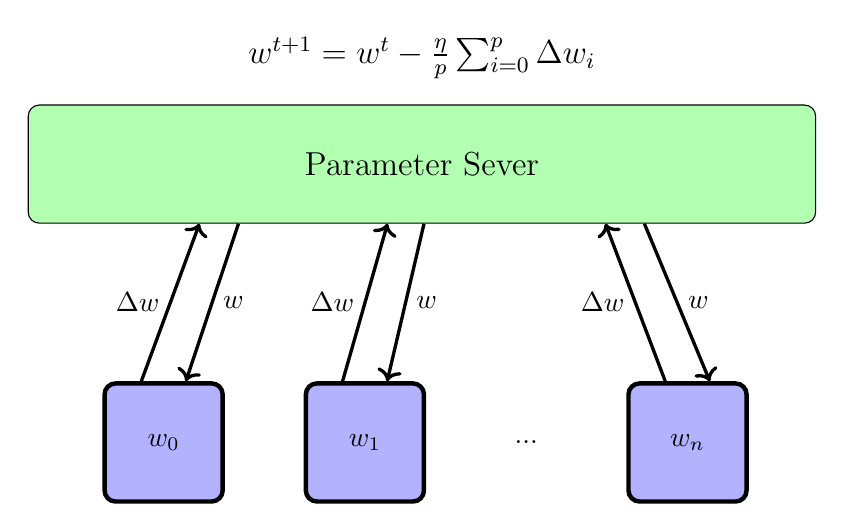
\begin{tikzpicture}[
        wkrsty/.style={
            rounded corners, ultra thick,
            draw, rectangle,
            minimum height=1.5cm,
            minimum width=1.5cm,
            fill=blue!30,
        },
        svrsty/.style={
            font=\large, fill=green!30,
            draw, rectangle, rounded corners,
            minimum height=1.5cm,
            minimum width=10cm,
        },
        arrowsty/.style={->, very thick},
        msgsty/.style={midway},
    ]
    
    \node[svrsty] at (0,0) (svr) {Parameter Sever};

    \node[above=0.2cm of svr, font=\large] {$w^{t+1} =w^t - \frac{\eta}{p} \sum^{p}_{i=0}\Delta w_i$};
    
    \node[wkrsty,below=2cm of svr.193] (w0) {$w_0$};
    \node[wkrsty, right=of w0] (w1) {$w_1$};
    \node[right=of w1] (dots) {...};
    \node[wkrsty, right=of dots] (wn) {$w_n$};

    \draw[arrowsty] (w0.110) -- node[msgsty,left] {$\Delta w$} (svr.195);
    \draw[arrowsty] (svr.198) -- node[msgsty,right] {$w$} (w0.70);
    
    \draw[arrowsty] (svr.272) -- node[msgsty,right] {$w$} (w1.70);
    \draw[arrowsty] (w1.110) -- node[msgsty,left] {$\Delta w$} (svr.240);
    
    \draw[arrowsty] (wn.110) -- node[msgsty,left] {$\Delta w$} (svr.342);
    \draw[arrowsty] (svr.345) -- node[msgsty,right] {$w$} (wn.70);

    \end{tikzpicture}
    
    \caption[Paramater Server Architecture]{
    Outline of a parameter server architecture for data parallelism.
    Blue squares represent workers who perform training, and green squares represent the parameter server that manages the ground truth of the model.
    Workers receive a set of weights from the server, perform SGD to calculate weight updates, and contribute their updates to the parameter server.
    Adapted from \cite{Dean2012DistBelif}}
    \label{fig:param_svr_arch}
\end{figure}



To eliminate the parameter server, a decentralized approach must be taken.
To accomplish this, the parameter server's jobs of aggregating, averaging, and distributing the model update can be replaced by an allreduce operation.
Caffe was the first software package where many of these ideas were evaluated, see Figure \ref{fig:caffe-dp-arch}.
Early results demonstrated how adopting tree-based allreduce/broadcast techniques could lessen communication pressure \cite{Iandola2016FireCaffe}, and further work adopting \gls{HPC} techniques like communication/computation, improved data staging, and more sophisticated allreduce algorithms could significantly improve scaleability \cite{Awan2017SCaffe}.

\begin{figure}
    \centering
    \begin{tikzpicture}[
        nnodesty/.style={draw, circle, minimum width=0.5cm},
        psty0/.style={fill=blue!40},
        psty1/.style={fill=yellow!40},
        psty2/.style={fill=red!40},
        passtxtsty/.style={midway,sloped,below,font=\scriptsize},
        imgsty/.style={draw, rectangle, 
            minimum height=1cm,
            minimum width=1cm,
        },
        arrsty/.style={single arrow, rotate=-90,draw, minimum height=0.5cm, minimum width=0.5cm},
    ]
    
    \foreach \x in {0,1,2}
        \foreach \y in {0,1,2}
            \node[nnodesty,psty0] at (\x,\y) (n\x\y0) {};
            
    \foreach \x in {0,1,2}
        \foreach \y in {0,1,2}
            \node[nnodesty,psty1] at (\x+4,\y) (n\x\y1) {};
            
    \foreach \x in {0,1,2}
        \foreach \y in {0,1,2}
            \node[nnodesty,psty2] at (\x+8,\y) (n\x\y2) {};
            
    \foreach \nn in {0,1,2}
        \foreach \x in {0,1,2}
            \foreach \y in {0,1,2}{
                \draw (n\x0\nn) -- (n\y1\nn);
                \draw (n\x1\nn) -- (n\y2\nn);
            }

    \node[rectangle, draw, minimum height=0.5cm, minimum width=4cm] at (5,-4) (avgbuf) {$\Delta w = 1/p * \sum_{i=0}^p \Delta w_i$};
    \node[draw,rectangle, above=3.5cm of n121] (initw) {$w^{t+1} = u(w^t,\Delta w, t)$};

    \foreach \nn in {0,1,2}{
        \node[imgsty, psty\nn, above=of n02\nn,xshift=0.4cm,yshift=0.1cm] () {}; 
        \node[imgsty,psty\nn,above=of n02\nn,xshift=0.5cm] () {}; 
        \node[imgsty,psty\nn,above=of n02\nn,xshift=0.6cm,yshift=-0.1cm] () {}; 
        \node[arrsty,above=0.2cm of n02\nn, yshift=0.125cm, xshift=-0.25cm] (im\nn) {};
        
        \draw[->, very thick] (n02\nn) ++(-0.5, 0) -- node [passtxtsty] {Forward Pass} +(0,-2);
        \draw[->, very thick] (n20\nn) ++(0.5, 0) -- node [passtxtsty] {Backward Pass} +(0,2);
        \node[arrsty,below=0.2cm of n10\nn, yshift=0.325cm, xshift=0.25cm] (dw\nn) {};
        \node[rectangle, draw, minimum height=0.5cm, minimum width=2cm, below=of n10\nn] (dw\nn){$\Delta w_\nn$};  
        \draw[->] (dw\nn) -- node[midway,passtxtsty] {\texttt{MPI\_Reduce}} (avgbuf);

    }

    \draw[->](initw.200)-- ++(0,-0.5) -- ++(-2,0) -- node[midway,passtxtsty,above] {\texttt{MPI\_Bcast}} (n220);
    \draw[->](initw.270) -- ++(0,-0.5) -- ++(1,0) -- node[midway, passtxtsty,above] {\texttt{MPI\_Bcast}} (n221);
    \draw[->] (initw.345) -- ++(0,-0.5) -- ++(3.6,0) -- node[midway,passtxtsty,above] {\texttt{MPI\_Bcast}} (n222);

    \draw[->] (avgbuf.east) -- ++(4.5,0) -- node[midway, passtxtsty,below] {Apply weight updates} ++(0,10) --(initw.east);
    
    \end{tikzpicture}
    \caption[Decentralized Data Parallelism Implemented in Caffe]{
        Decentralized data parallel architecture of Caffe.
        Instead of direct updates to a parameter server, weight updates are reduced to some specified leader, and weights for the next round of training are broadcast.
        This allows for more optimal reduce/broadcast algorithms as opposed to the linear reduce/broadcast enforced by parameter servers.
        Adapted from \cite{Awan2017InDepthPerfCharOfDNN}
    }
    \label{fig:caffe-dp-arch}
\end{figure}

Some of the earliest work noted that load imbalance would significantly impact training performance. 
If any individual rank were significantly delayed, the entire training process would have to stall waiting for it to arrive.
This led to the idea of asynchronous training.
Thanks to its stochastic and iterative characteristics, the \gls{SGD} algorithm is resilient to model disruptions and can still converge even if work is lost or iterations take missteps.
Many researchers have proposed \gls{SGD} variations that break consistency assumptions to remove synchronization and increase performance.
Dean et al. \cite{Dean2012DistBelif} propose Downpour \gls{SGD}, a parameter server-based algorithm where workers only send $\Delta w$ during synchronization and infrequently receive a local copy from the parameter server so as not to deviate too far from the global model. 
Recht et al. \cite{Recht2011HogWild} take it a step further and demonstrate that \gls{SGD} does not need any synchronization at all, the authors show that a pool of workers can update global weights in an \gls{SMT} environment without any locking mechanisms.
Their algorithm, which they call Hogwild, shows how data loss due to race conditions does not adversely affect training.
Noel and Osindero extend this idea to a distributed environment with Dogwild \cite{Noel2014Dogwild}.

Asynchronous training was initially proposed for, and is implemented on, parameter server architectures, but they do not entirely mitigate the scaling issue of centralized systems.
Adapting asynchronous training methods to decentralized training is more difficult, as existing allreduce methods only support synchronous training, however this has not stopped researchers from trying.
Using an \gls{MPI}-based distributed training library, Kurth et al. proposed gradient lag, a method where weight updates are an iteration behind, i.e. Line 7 in Algorithm \ref{alg:MinibatchSGD} becomes $w^{(t+1)}\leftarrow w_{mb} + \Delta w^{(t-1)}$, to increases computation/communication overlap, and allow training to utilize large scale systems fully \cite{Kurth2018ExascaleDLClimate}.
Li et al. propose the concept of partial collectives, which require a subset of the processes to synchronize instead of the entire communicator \cite{Li2020DLPartialColl}.
If any process takes too long to arrive, its values from the previous allreduce are used, this lessens the required synchronization while maintaining enough training stability to promote convergence.

While loosening the constraints of minibatch \gls{SGD} can lower synchronization and increase performance, it requires technical expertise in both \gls{HPC} communication and \gls{DL} training, making the barrier to entry incredibly costly.
Often, techniques are built on standardized \gls{HPC} libraries, so there is a vested interest for legacy \gls{HPC} researchers to adapt existing methods to emerging \gls{DL} methods.

\subsection{Collective Optimizations for Deep Learning}
There are a plethora of \gls{DL} libraries that support distributed data-parallel DL.
Earlier methods would rely on explicit reduce/broadcast operations to achieve the desired effect, but over time more performant techniques and optimizations were proposed and incorporated.
Modern model parallel \gls{DL} tools have a broad set of design targets, including leveraging high-performance allreduce algorithms, overlapping as much communication and computation as possible, and load balancing the workload across the cluster.
However, the running theme through all this research is that data-parallel training is highly reliant on large-message \gls{GPU}-based allreduce. 

Caffe was one of the first libraries to provide data-parallel training and was a proving ground for allreduce techniques in \gls{DL}.
Awan et al. \cite{Awan2017InDepthPerfCharOfDNN} identify a handful of issues with Caffe, including the bulk-synchronous-parallel structure and lack of efficient communication, and they demonstrate that preexisting \gls{MPI} algorithms can greatly improve performance.
In further work, they propose S-Caffe \cite{Awan2017SCaffe}, a fork adapted for scalability that leverages non-blocking operations to increase overlap and propose a \gls{DL}-targeted hierarchical \texttt{MPI\_Reduce} for large \gls{GPU} buffers.

Cho et al. \cite{Cho2019BlueConnect} propose their own hierarchical topology-aware allreduce algorithm for large \gls{GPU} buffers, which they dub BlueConnect. 
Their method decomposes \gls{RSA} into multiple reduce-scatters and allgathers and maps each pair of collectives to a layer in the cluster's hierarchy.
They evaluate their work by embedding it in Caffe2, demonstrating \gls{DL}'s reliance on large message allreduce.

Bayatpour et al. \cite{Bayatpour2018SALaR} design a pipelined hierarchical allreduce algorithm for large messages on \gls{CPU} systems, with a focus on overlapping the internode and intranode stages to maximize utilization, and the bandwidth usage improvements showed increased performance on multiple \gls{DL} frameworks including \gls{CNTK} and Horovod. 

Chu et al. \cite{Chu2020NVGroup} propose a similar algorithm with support for \gls{GPU}s, which also shows increased Horovod performance.
To maximize the usage of intranode resources, their method leverages persistent kernels, this allows them to saturate NVLink while seamlessly performing the local reduction, significantly increasing overall performance. 
To integrate the \gls{GPU} kernel-based communication with the network, the authors define a communication management engine that pipelines data between the intranode and internode stages.

Proposed \gls{DL}-focused allreduce algorithms tend to leverage a common set of tools, including hierarchical structures, pipelining, and \gls{GPU}-based reductions.
The hierarchical structure is a form of implicit topology awareness and ensures that the most performant interconnect are used as much as possible.
Pipelining allows the overlap of multiple types of communication if resources can shuffle data concurrently, this lower overall allreduce latency. 
\gls{GPU}-Kernels greatly diminish the time spent performing local reduction computations, and while there is a penalty in the form of host-to-device copies, these can be designed around and hidden.
Therefore, future large-message algorithms should attempt to leverage these techniques where possible to maximize performance. 

Outside of raw performance, there are other angles to tackle allreduce performance.
Since process imbalance can be an issue with \gls{DL}, there have been attempts to mitigate the impact of synchronization using \gls{PAP} awareness.
Proficz proposes a \gls{PAP} estimation method \cite{Proficz2018ImprvAllReduceForImbPAP} targeting allreduce.
As the application approaches the collective, it notifies the \gls{MPI} runtime that synchronization is imminent, which allows the library to construct a collective schedule minimizing process idle time, and the author demonstrates how \gls{PAP} awareness can accelerate training on CFIAR-10.
Alizadeh et al. \cite{Alizadeh2022PAPCollDL} analyze the impact of process imbalance on Horovod and demonstrate that allreduce operations are frequently subject to process arrival imbalance. 
Further, they demonstrate that hierarchical algorithms are more imbalance tolerant than flat algorithms and that hierarchical algorithms can increase training throughput.

A handful of methods leverage characteristics specific to \gls{DL} to increase communication efficiency.
Key observations include gradient update sparsity and \gls{SGD}'s ability to recover from missteps during training.
Renggli et al. \cite{Renggli2019SparCML} proposed a communication method that leverages gradient sparsity to minimize the amount of data communicated.
They encode update vectors as a set of index/value tuples which can significantly compress update vectors depending on the amount of sparsity.
To apply their work to \gls{DL}, the authors define an allreduce algorithm that can adaptively switch between sparse and dense data representation as sparsity decreases during the allreduce operation and validate their work by integrating it within \gls{CNTK}.
Dryden et al. \cite{Dryden2016CommQuantDPDNN} combine update sparsity with \gls{SGD} resilience to propose adaptive quantization. 
Quantization is a method for encoding 32-bit values as a single-bit, the authors' method selects a portion of the update values and sends a vector of 32-bit values where bit 31 is the update indicator and bits 30-0 are the value's index.
They implemented their work in LBANN and demonstrated that they could achieve increased performance without sacrificing accuracy.

Another handful of ideas involves breaking the constraints of \gls{MPI}.
As mentioned before, Li et al. \cite{Li2020DLPartialColl} proposed partial collectives, which lower synchronization by only requiring a subset of a communicator to contribute to the allreduce. 
Dryden et al. \cite{Dryden2018Aluminum} identified that \gls{MPI} is unaware of \gls{GPU} streams, forcing application developers to use overly-heavy synchronizations when moving data between MPI and \gls{CUDA}.
Their proposal, Aluminum, is a collective library that accepts a \gls{CUDA} stream when performing non-blocking allreduce operations and does an efficient job mitigating synchronization issues between \gls{MPI} and \gls{CUDA}.
They also validate their library by demonstrating improved strong and weak scaling of LBANN.

\subsection{Horovod}\label{sec:CH3-horovod}
The most widely used library for orchestrating data-parallel training is Horovod \cite{Sergeev2018Horovod}, its popularity is derived from its ease of use since it builds on top of existing \gls{DL} frameworks like TensorFlow and Pytorch and how it uses efficient collective libraries like \gls{MPI} and \gls{NCCL}.
Horovod has been widely adopted in the \gls{DL} community, and the \gls{MPI} community has used it as a target for optimization.
Horovod has been shown to be capable of tackling immense scale and fully utilize some of the world's largest systems, like 8000 Xeon Phi nodes on Cori \cite{Mathuriya2019Cosmoflow}, or 4000 V100 nodes on Sumit \cite{Kurth2018ExascaleDLClimate}.

Horovod builds on top of existing \gls{DL} libraries, hooking into internal data representations to seamlessly provide scalability.
\gls{DL} frameworks internally represent the model as a \gls{DAG}, where vertices are layers and edges represent the data flow between layers, 
At runtime, \gls{DAG} elements are scheduled on an execution engine which maps the computations and dataflow to the available hardware.
To maximize performance, operations can be issued in any order, and this can differ between runs of the same network \cite{Abadi2015TensorflowWhitepaper}. 
Horovod ties into existing \gls{DL} frameworks by hooking into the internal \gls{DAG} through a \textit{distributed optimizer} object, which embeds allreduce operations on the appropriate \gls{DAG} vertices.

All communication is issued on a background thread to increase compute/communication overlap.
However, allreduce operations in \gls{MPI} require strict ordering, so when there is a potential race between two layers like in Figure \ref{fig:ResNet-controll-dependency}, Horovod must determine which ranks have finished which layers to schedule allreduces accordingly \cite{Kurth2019TFatScaleAnalysisOfHvdAndCPEML}.  
To determine which layers are ready, the communication thread performs a bitwise and allreduce on a bit-vector where each bit represents a layer.
This check happens continuously through training generating frequent small size (order of 8B) \gls{CPU}-based allreduces.
When all ranks have agreed upon a set of layers to average, the weight updates are packed into a buffer (known as the tensor fusion buffer), a large (order of 64MB) \gls{GPU}-based allreduce is issued, and the reduced result is copied back into the appropriate data location.
Profiling of Horovod by Alizadeh et al. \cite{Alizadeh2022PAPCollDL} echos this communication pattern, with a mix of frequent small \gls{CPU}-based allreduces and large \gls{GPU}-based allreduce operations.

\begin{figure}
    \centering
        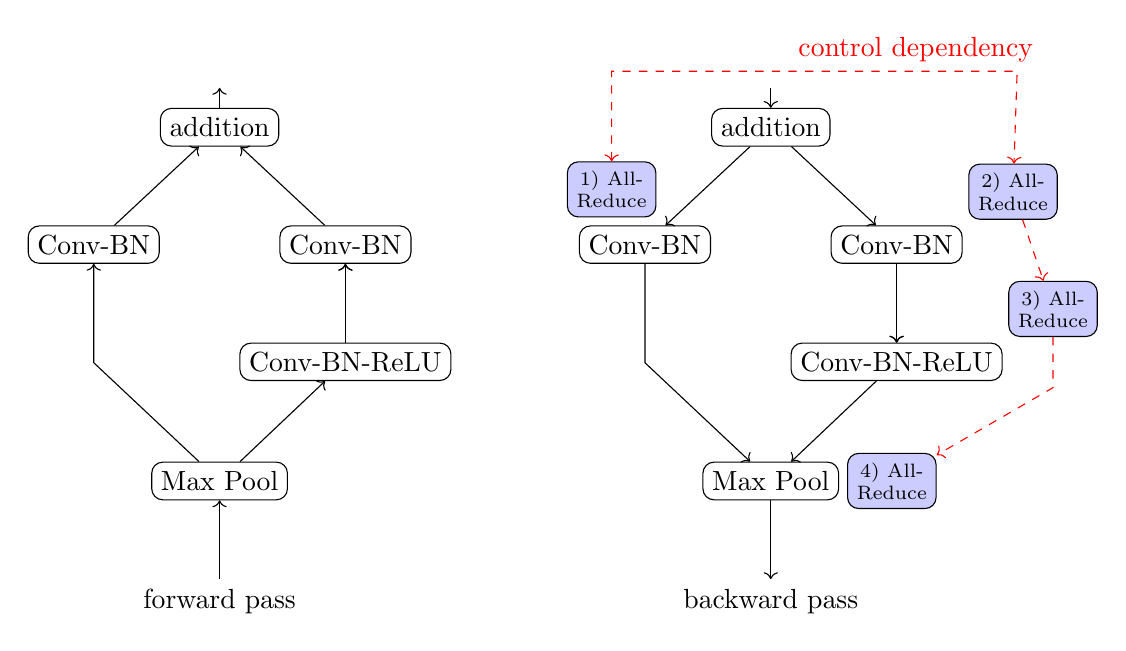
\begin{tikzpicture}[
        elemsty/.style={
            draw, rectangle, rounded corners,
        },
        cdsty/.style={
            draw, fill=blue!20,align=center,rounded corners,
            font=\scriptsize,
        },
        cdlinesty/.style={
            red,dashed
        }
    ]
    
    \foreach \x in {0,1}{
        \node[elemsty] at (\x*7,0) (add1\x) {addition};
        \node[elemsty,below left=of add1\x, xshift=1cm] (convbn1\x) {Conv-BN};
        \node[elemsty,below right=of add1\x, xshift=-1cm] (convbn2\x) {Conv-BN};
        \node[elemsty,below=of convbn2\x] (convbnrelu1\x) {Conv-BN-ReLU};
        \node[elemsty,below=4cm of add1\x] (mp1\x) {Max Pool};
    }
    \node[below=of mp10] (fp) {forward pass};
    \node[below=of mp11] (bp) {backward pass};

    \draw[->] (fp) -- (mp10);
    \draw[->] (mp10) -- (convbnrelu10);
    \draw[->] (convbnrelu10) -- (convbn20);
    \draw[->] (convbnrelu10) -- (convbn20);
    \draw[->] (convbn20) -- (add10);
    \draw[->] (convbn10) -- (add10);
    \draw[->] (add10) -- +(0,0.5);
    \draw[<-] (convbn10) -- +(0,-1.5) -- (mp10);
    
    \draw[<-] (bp) -- (mp11);
    \draw[<-] (mp11) -- (convbnrelu11);
    \draw[<-] (convbnrelu11) -- (convbn21);
    \draw[<-] (convbnrelu11) -- (convbn21);
    \draw[<-] (convbn21) -- (add11);
    \draw[<-] (convbn11) -- (add11);
    \draw[<-] (add11) -- +(0,0.5);
    \draw[->] (convbn11) -- +(0,-1.5) -- (mp11);

    \node[cdsty, above=0.1cm of convbn11.150] (cd0) {1) All-\\Reduce};
    \node[cdsty, above right=0.1cm of convbn21] (cd1) {2) All-\\Reduce};
    \node[cdsty, above right=0.1cm of convbnrelu11] (cd2) {3) All-\\Reduce};
    \node[cdsty, right=0.1cm of mp11] (cd3) {4) All-\\Reduce};

    \draw[<->,cdlinesty] (cd0) -- ++(0,1.5) -- node[above,near end] {control dependency} ++(5.15,0) -- ++(cd1);
    \draw[->,cdlinesty] (cd1) -- (cd2);
    \draw[->,cdlinesty] (cd2) -- ++(0,-1) -- (cd3);
        
    \end{tikzpicture}
    \caption[Ambiguity in ResNet Block Operation Ordering]
    {ResNet blocks generate ambiguity in terms of reduction order.
    Distributed DL frameworks must handle allreduce ordering in order to avoid deadlocks and data corruption.
    Figure adapted from \cite{Li2020DLPartialColl}}
    \label{fig:ResNet-controll-dependency}
\end{figure}


There are tunable environment variables that can affect the communication performance of Horovod.
\texttt{HOROVOD\_CYCLE\_TIME} manages the frequency with which the fusion buffer is flushed, it accepts a value in milliseconds denoting the period between \gls{GPU} allreduce calls.
\texttt{HOROVOD\_FUSION\_THRESHOLD} specifies the size of the tensor fusion buffer, by default, it is set to 64MB, but this can be increased to generate larger allreduce operations.
Further, the fusion buffer can be set to 0, which effectively disables the fusion buffer.
This replaces a few large allreduce operations with several smaller allreduce operations but can show improved performance depending on the underlying hardware \cite{Awan2019CommProfDLonClusters}.

\section{Conclusion}
Over the past decade \gls{ML} and \gls{DL} have exploded in popularity, with more powerful models being deployed across a vast set of domains.  
However, as \gls{DL} research advances, there is a constant desire to train larger models on bigger datasets.
In order to accommodate the ever-increasing need for compute, we can use weak scaling to train large-scale \gls{DL} models on highly parallel systems in a reasonable amount of time.

The foundations of \gls{ML}, namely \gls{SGD} and neural networks, have existed for decades, and there are several methods of decomposing the problem across compute resources.
We outline three strategies, hyperparameter search, model parallelism and data parallelism.
Each method targets a different aspect of \gls{DL} and generates its own unique communication patterns.
Hyperparameter search evaluates different architectures in parallel and often relies on a central server to manage the search algorithm. 
Model parallelism distributes chunks of the network across resources and generates all-to-all collectives as \gls{GEMM} operations are performed across distributed memory.  
Data parallelism leverages concurrency in minibatches to iterate through the dataset more efficiently.
Initial data parallel training frameworks would rely on a parameter server, however, this has become a chokepoint for scaling, and modern systems heavily rely on allreduce operations. 

At this point in time, data parallelism is the most well-understood strategy, and production-ready libraries like Horovod are in wide use today.  
We break down some of the design characteristics of Horovod, outline how large message \texttt{MPI\_Allreduce} can limit performance, and highlight existing works that attempt to alleviate this issue.
The next two chapters of this thesis each propose a new allreduce algorithm.
Both algorithms target large message \gls{GPU} allreduce, and even though they use two different approaches, both algorithms are designed with the goal of improving Horovod's performance.

\clearpage
% Chapter 4 - Topology Awareness

\glsresetall % reset the glossary to expand acronyms again
\chapter[Topology]{Topology Awareness}\label{ch:TopologyAwareness}
\index{Topology Awareness}

% Topology Awareness

\begin{itemize}
    \item Horovod, even though there's barely any improvement?
\end{itemize}

The first technique investigated to improve MPI collective communication performance is topology awareness.
The overarching idea is to accelerate computation by leveraging the knowledge of the underlying hardware.
Topology awareness is an often-used technique applied to many areas in both MPI and the greater HPC ecosystem.

This chapter builds on work by Mirsadeghi and Afsahi \cite{Mirsadeghi2016TopoAwareCollRR}, where the authors propose a method for applying topology awareness to allgather and broadcast.
Their work relies on the notion that collective algorithms have an implicit communication pattern and that the ranks in a communicator can be reordered to better fit the communication pattern to the host topology.
We start by extending their work to multiple new algorithms in allreduce and broadcast.
Microbenchmark evaluation shows that we can see up to 80\% performance improvement under certain scenarios, and our proposed mapping heuristics can outperform the established SCOTCH graph partitioning library \cite{Pellegrini2012SCOTCH}.

This chapter will start by outlining existing methods for applying topology awareness within MPI.
Next, we propose a method of accelerating MPI collectives and build an implementation targeting multiple MPI\_Allreduce and MPI\_Bcast algorithms.
Our work is evaluated in both CPU and GPU environments and on a fat-tree cluster.

\section{Motivation}
MPI provides a programming model so that processes on a distributed memory system can share data and work together.
MPI users are meant to assume that messages exchanged between any two ranks will have the same communication characteristics no matter what their ranks are. 
This abstraction provides a convenient programming environment allowing users to focus on building their application without worrying about the underlying hardware. 
Its simplicity also has the benefit of making portability easier, dissuading users from tying their application to a specific architecture.
But in reality, this assumption is false because modern computers are anything but simple. 
Compute nodes have expansive memory hierarchies spanning multiple caches, NUMA domains, and even GPU memory.
Furthermore, modern fabric interconnects have complex network topologies with variable performance depending on node location.
So, in reality, the hardware topology of the system has an outsized impact on message performance, which has a knock-on effect on overall application performance. 

MPI applications often have consistent and predictable data-transfer patterns, this means any one rank will often send and receive the same set of messages to and from the same set of peers on consecutive runs of the application.
Since data-transfer patterns are predictable, and the programming model doesn't bind processes to specific locations, this gives MPI implementations the flexibility to map ranks to processing elements to make the most optimal use of the underlying hardware.
This problem of mapping ranks to processing elements can be formalized as an instance of a graph-embedding problem. However, previous work has shown this to be an NP-Hard problem \cite{Hoefler2011GenericTopoMappingStrats}. 
Solving this problem at scale (on the order of millions of processes) is not feasible. Therefore heuristics and simplifications are often used instead.

To apply topology awareness to collectives, we can leverage how collective algorithms are structured as a series of point-to-point communications.
MPI providers will often include multiple algorithms for different collectives with common patterns, including ring, recursive doubling, knomial-tree, etc...
This gives MPI implementations the flexibility to select a performant algorithm depending on the collective's parameters like message size and the number of processes.
This framework for algorithm selection neglects the host topology, but there is room to incorporate it.
The collective algorithm defines the pattern to disseminate data, but the value of the ranks in the graph often does not matter (there are some algorithms where this does matter, like allgather, alltoall and commutative allreduce, but these can be accounted for).
So in this work, we evaluate the efficacy of mapping collective communication graphs to the underlying hardware topology on-the-fly during application runtime.

\section{Related works}
Topology awareness is a commonly used technique for accelerating MPI applications. 
Within MPI, there are many scenarios and methods where topology information can be applied to accelerate communication.
At the highest level, topology awareness can be applied to the application's entire communication graph \cite{Hoefler2011GenericTopoMappingStrats, Mirsadeghi2016PTRAM, Faraji2016TopoAwareGPUSelection, Mirsadeghi2016MAGC, Galvez2017AutoTopoMap}.
These strategies require profiling the entire application to build the communication graph.
This communication graph is then used in future runs of the application to devise a mapping for each job allocation.
The efficiency of a mapping is evaluated using metrics such as hop-bytes or congestion.
So to achieve the best application performance, mapping algorithms try to minimize/maximize their chosen metric.
There are multiple research fronts with this strategy, efforts have gone into optimizing the metrics, the mapping algorithm itself, and the types of systems mappings are supported for.

Hoefler and Snir \cite{Hoefler2011GenericTopoMappingStrats} propose a general process mapping tool targeting CPU clusters.
They evaluate three algorithms, a greedy algorithm based on vertex weights, a recursive bisecting that makes minimum weighted edge-cuts, and a graph similarity mapping using the Reverse Cuthill McKee algorithm. 
They use these algorithms, along with a \textit{Threshold Accepting} optimization step, to minimize congestion and dilation on large-scale SMP clusters.

Mirsadeghi and Afsahi \cite{Mirsadeghi2016PTRAM} propose a system targeting large-scale Infiniband clusters.
Their system leverages the network topology plus Infiniband's static routing tables to further reduce congestion.
They propose a hybrid metric which is a linear combination of hop-bytes and three types of congestion statistics. 
The mapping, along with further refinements, are calculated using a parallel greedy algorithm.

Faraji et al. l \cite{Faraji2016TopoAwareGPUSelection} focus their efforts on building a system targeting intranode GPU communication.
While their system only works on a single node and relies on SCOTCH's \cite{Pellegrini2012SCOTCH} graph bisecting method to perform the mapping, Mirsadehi et al. \cite{Mirsadeghi2016MAGC} expand the work to a full cluster.
The complete system uses a 3-step process, first mapping ranks to nodes to minimize network communication, then ranks to core to optimize intranode communication, and lastly, the GPU-to-rank step for optimal GPU-to-GPU communications.

Existing systems struggle to manage collective communications.
The profiling stage is often built on top of the PMPI profiling interface, which can intercept MPI calls, but doesn't break collectives into their constituent point-to-point messages.
Galvez et al. \cite{Galvez2017AutoTopoMap} identify this problem and propose a profiler that groups types of communications into weighted classes.
Their system leverages a parallel algorithm that uses the communication classes, along with a set of weighted metrics, to calculate a near-ideal mapping.
While a step in the right direction, their solution still treats collective communications as a black box, focusing on the collective's communicator and not disassembling the collective into its constituent point-to-point messages.

In order to decompose collectives into point-to-point messages, Bosilica et al. \cite{Bosilica2017OnlineMonitoringMPI} implemented a monitoring layer in OpenMPI that is accessible through the MPI Tools interface.
This provides much more granular profiling for point-to-point messages, which allowed Jeannot and Sartori \cite{Jeannot2020ImprvMPICommMonitoring} to propose a rank reordering method for applications with iterative compute, but their solution is required to be implemented within the user's application. 
So while it is possible to apply topology awareness to all communication, including collectives, there is a large burden on application developers to implement it within their software.

One of the common shortcomings most of these systems have in common is the required application profiling.
The application needs to run at least once to build the communication graph, and this can be expensive for large-scale runs. 
An ideal solution would be able to build a graph for a moderate amount of processes and project a solution for a large-scale system, but no existing solution can perform this yet. 

The MPI standard does provide a few interfaces to allow application developers to inform the runtime of expected communication patterns.  
One of these solutions are virtual topologies. 
This is a structure attached to a communicator that tells the implementation how communications are likely to occur between ranks.
Mercer and Jeannot \cite{Mercer2011ImprvMPIWithRR} leverage the MPI\_Dist\_graph\_create endpoint to reorder processes on a graph topology.
Their solution centralizes the topology information and uses the TreeMatch algorithm \cite{Jeannot2010TreeMatch} to calculate a process reordering.
Gropp \cite{Gropp2019CartTopoMapping} proposes a method for reordering processes in a cartesian topology.
His method relies on MPI\_COMM\_TYPE\_SHARED and neglects network topology as well as memory hierarchy information.

The most common way to apply topology awareness within collectives is to use a hierarchical strategy.
This is done by splitting the communicator into intra-node and inter-node sub-communicators.
The intra-node communicator consists of processes that are all placed on the same node.
Each node selects a leader process which is a member of the inter-communicator.
The collective communication pattern is then implemented across the hierarchical structure, ensuring efficient hardware use between shared memory and network resources.

Lue et al. \cite{Luo2018ADAPT} propose a library for event-based collectives.
While the crux of their work is focused on minimizing synchronization dependencies within collectives, they do demonstrate how their work could easily be mapped to a hierarchical type algorithm.
Awan et al. \cite{Awan2016NCCLBcast} build a GPU-aware hierarchical bcast algorithm.
Their work leverages NCCL for optimal intra-node communication for large messages and relies on existing algorithms in MVAPICH2 for inter-node communication.

Subramoni et al. \cite{Subramoni2011SpeedAwareBcast} designed a broadcast algorithm that can take Infiniband topology and network speeds into account.
They gather network information using OFED management tools like ibnetdiscover and ibroute and use the information to build a reordered communicator using either a depth-first traversal or a breath-first traversal.
They only evaluate knomial and scatter-allgather collectives.

The work presented in this thesis is an extension of work by Mirsadeghi and Afsahi \cite{Mirsadeghi2016TopoAwareCollRR}.
Instead of building a communication graph to custom fit the host topology, this work leverages the existing algorithm but renumbers the ranks under the hood to better map the communication graph to the hardware.
Their work focuses on broadcast and allgather collectives, with remapping algorithms targeting ring, recursive doubling and binomial communication patterns.
We extend their work by looking at allreduce and the additional challenges the reduction operation adds to their method.
We also propose mapping algorithms for reduce-scatter-allgather, knomial and binary-tree communication patterns.

\section{Method}
When applying topology awareness to collectives there are two common strategies.
Either build a communication pattern that is designed to fit the hardware or take an existing pattern and efficiently map it to the hardware.
This work uses the latter strategy, we take the collective algorithm selected by the implementation and silently renumber the processes to better utilize communication resources.
When a collective is called, the MPI library selects an algorithm based on the message size and number of processes.
The communication pattern is implicit to the collective algorithm, so we define a heuristic tailored to specific algorithms that calculate how ranks should be renumbered.
To make the calculation efficient and scalable, each proposed remapping heuristic leverages a greedy strategy, and an outline of the general strategy is given in algorithm \ref{alg:toporr-strat}.
The basic structure starts with a reference rank, all process remappings will try to use hardware as close to the reference rank as possible.
Then the heuristic loops through the ranks, selecting the next rank to map based on the communication pattern, updating the reference rank when required.

The mapping is enforced by creating a new communicator.
Each process calls MPI\_Comm\_split() requesting their new rank, and then the selected algorithm is run on the resulting communicator.
Since communicator creation is an expensive operation, this shadow communicator is cached so that it can be used again if the same communicator uses the same algorithm.

This structure is flexible and allows us to evaluate multiple types of collectives.
Mirsadeghi and Afsahi \cite{Mirsadeghi2016TopoAwareCollRR} propose heuristics targeting ring allgather, recursive doubling allgather, and binomial tree broadcast. 
We reimplement their ring and recursive doubling algorithms and evaluate them on allreduce collectives, and evaluate their binomial-broadcast heuristic in the context of a scatter-allgather broadcast.
To extend their work while targeting large message allreduce, we propose a new reordering heuristic for reduce-scatter-allgather allreduce.
Furthermore, since broadcast can be used as a component in allreudce, we also propose heuristics for two broadcast algorithms, knomial and binary tree broadcast.

% \lstset{style = bklstc}
% \lstset{label = lst:topo-generic-strategy}
% \lstset{caption = General greedy heuristic for topology-aware rank reordering.}
% \lstinputlisting[float=!htbp]{3_Chapters/4_Chapter_TopologyAwareness/Figures/TopoRR_strat.c}
\begin{algorithm}
    \caption{General Mapping Heuristic Strategy}
    \label{alg:toporr-strat}
    \begin{algorithmic}[1]
        \Require Number of Processes $p$, physical topology distance matrix $D$
        \Ensure  Mapping array $M$ representing the new rank for each process
        \State Bind rank 0 to its current core
        \State Set rank 0 as the reference rank
        \While{There are processes to map}
            \State Select the target rank to map
            \State Find an unmapped core with the minimum distance to the reference core  
            \State Bind the target rank to the selected core
            \State Optionally update the reference core
        \EndWhile
    \end{algorithmic}
\end{algorithm}

\subsection{Reduce-Scatter-Allgather Allreduce}
Reduce-scatter-allgather (RSA) allreduce, also known as Rabenseifner's algorithm, is a popular algorithm implemented in most MPI implementations and even used in external collective libraries like UCC \cite{UCC}.
The algorithm starts with each process performing a recursive-vector halving reduce-scatter, this distributes a segment of the fully reduced vector to each rank.
At this point, each rank needs to gather the other reduced segments from the other ranks, this is achieved through a recursive doubling allgather.
RSA is used for large message allreduce because it efficiently uses system bandwidth.
For an allreduce with $p$ processes on $n$ bytes of data, each rank sends $2((p-1)/p)n\beta$ bytes of data, linear scaling with message size is ideal for large message collectives.
In terms of structure, since both phases rely on a recursive pattern, data is only exchanged with ranks that are a power of 2 distance away.
The other important feature of RSA is that more data is exchanged with numerically closer ranks.
Figure \ref{fig:graph-rsa} demonstrates this phenomenon with eight processes.
Most data is exchanged with immediate neighbours, this accounts for the first stage of reduce-scatter and the last stage of the allgather.

So while designing our heuristic, we want to map communicating pairs that are a power of two distances away, focusing on small distances first.
With these goals in mind, we propose the heuristic in algorithm \ref{alg:rsa} to target the RSA algorithm.
This heuristics starts by mapping rank 0 (line 1), then walks to the power of 2 communication graph mapping processes that have not been mapped yet (lines 5-10). 
While looping through all the ranks, the reference rank is updated every two mappings (lines 11-14), this ensures that communicating pairs that are distance one away are mapped as close as possible. 

% RSA
\begin{figure}
    \centering
    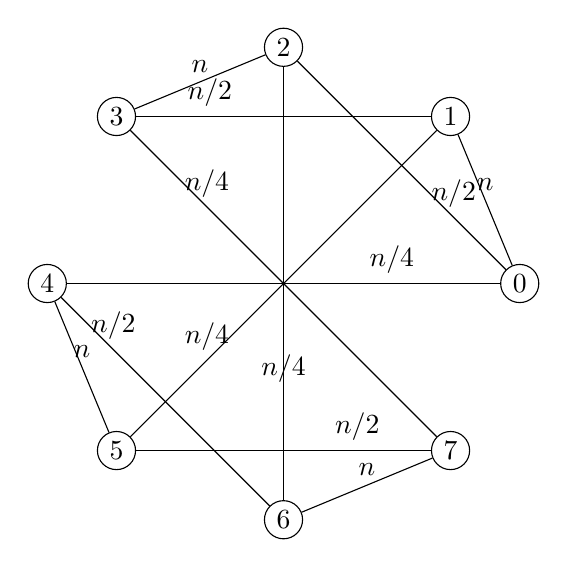
\begin{tikzpicture}
        \def\mycircleofnodes{C0}
        \foreach \x in {0,1,...,7}
            {
                \node[circle,draw,inner sep=2pt] (C\x) at (\x*45:3) {\x} ;
                \ifnum\x>0\relax\xdef\mycircleofnodes{\mycircleofnodes,C\x}\fi
            }

        \foreach \x/\y in {0/1, 2/3, 4/5, 6/7}
            {
                \draw (C\x) -- (C\y) node [above, midway] {$n$};
            }
        \foreach \x/\y in {0/2, 3/1, 4/6, 7/5}
            {
                \draw (C\x) -- (C\y) node [above, near start] {$n/2$};
            }
        \foreach \x/\y in {0/4, 5/1, 6/2, 3/7}
            {
                \draw (C\x) -- (C\y) node [above, near start] {$n/4$};
            }
    \end{tikzpicture}
    \caption{Eight process reduce scatter allgather, where message size is $n$.}
    \label{fig:graph-rsa}    
\end{figure}

% \lstset{label = lst:topo-rsa}
% \lstset{caption = Heuristic for rank reordering the reduce-scatter-allgather algorithm.}
% \lstinputlisting[float=!htbp]{3_Chapters/4_Chapter_TopologyAwareness/Figures/Topo_RSA.c}
\begin{algorithm}
  \caption{Reduce Scatter Allgather Heuristic}
  \label{alg:rsa}
  \begin{algorithmic}[1]
    \Require Number of processes p, physical topology distance matrix D
    \Ensure  Mapping array M representing the new rank for each process

    \State M[0] = 0;
    \State ref\_rank = 0;
    \State mask = 1;
    \While {\textit{there exist more processes to map}}
      \While {\textit{ ref\_rank $\oplus$ mask is already mapped }}
        \State mask *= 2;
      \EndWhile
      \State new\_rank = mask $\oplus$ ref\_rank;
      \State target\_core = find\_closest\_core(ref\_rank, D);
      \State M[new\_rank] = target\_core;
      \If {\textit{two processes have been mapped close to ref\_rank}}
        \State ref\_rank = new\_rank;
        \State mask = 1;
      \EndIf
      \EndWhile
  \end{algorithmic}
\end{algorithm}

\subsection{Binary Tree Broadcast}
Binary trees benefit from their simplicity.
Ranks receive one message and forward it to two child ranks.
The tree structure provides logarithmic scaling to the number of messages sent, so binary trees are often used for smaller message sizes. 
A typical structure for a binary tree is provided in Figure \ref{fig:graph-bin-tree}.
For a rank $r$, the height in the tree can be calculated as $h_r = \lfloor log_2(r+1) \rfloor$, and ranks will send messages to $r + 2^{h_r}$ and $r + 2^{h_r + 1}$
This leads to a structure where processes further down the tree are send messages to ranks further and further away.
Furthermore, binary trees are constructed slightly lopsided,  as nodes are added to the left side of the tree before the right side. 
This can lead to situations where one direction has slightly more nodes than the other, this should be accounted for when designing the heuristic.

To ensure that ranks reside on the same node as their children, we propose a depth-first-traversal heuristic with the code provided in algorithm \ref{alg:bintree}.
We employ a recursive function to traverse the tree efficiently. 
We start by mapping the tree's root (line 1) and passing it in as the reference rank to the recursive function (line 2).
The recursive function starts by calculating the reference rank's height and child processes (lines 4-7). 
Then, depending on if the child processes are in the communicator, we bind them close to the reference rank and recuse with the new process set as the reference rank (lines 8-15).
To account for lopsidedness, the heuristics traverses the potentially smaller side first by mapping the numerically greater child first.
We found that this does a more consistent job mapping the tree to system architectures we evaluated on.

\begin{figure}
    \centering
    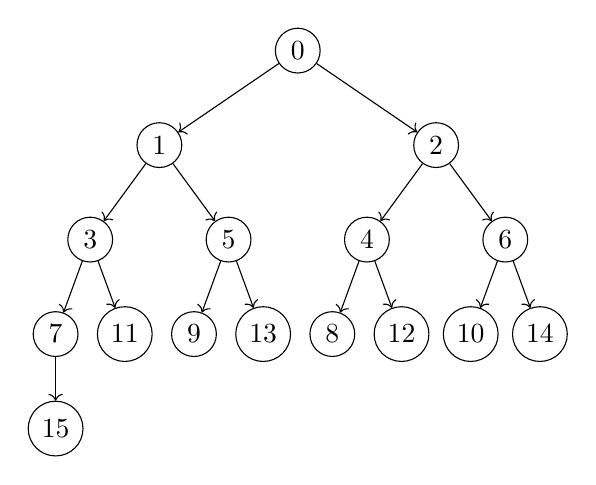
\begin{tikzpicture} [every node/.style = {shape=circle, draw, align=center}, inner sep=1mm, level distance=12mm]
        \tikzstyle{level 1}=[sibling distance=10em]
        \tikzstyle{level 2}=[sibling distance=5em]
        \tikzstyle{level 3}=[sibling distance=2.5em]
        \node {0}
        child [->] { node {1}
                child { node {3}
                        child {node {7} child {node {15}}}
                        child {node {11}}
                    }
                child { node {5}
                        child {node {9}}
                        child {node {13}}
                    }
            }
        child [->] { node {2}
                child { node {4}
                        child {node {8}}
                        child {node {12}}
                    }
                child { node {6}
                        child {node {10}}
                        child {node {14}}
                    }
            };
    \end{tikzpicture}
    \caption[Sixteen process binary tree broadcast graph]{
        16 processes structured in a binary tree.
        Each process receives one message and sends two, and all messages are the same size.
    }
    \label{fig:graph-bin-tree}
\end{figure}

% \lstset{label = lst:topo-bintree}
% \lstset{caption = Heuristic for rank reordering binary trees.}
% \lstinputlisting[float=!htbp]{3_Chapters/4_Chapter_TopologyAwareness/Figures/Topo_BinTree.txt}
\begin{algorithm}
  \caption{Binary Tree Heuristic}
  \label{alg:bintree}
  \begin{algorithmic}[1]
    \Require Number of Processes p, physical topology distance matrix D
    \Ensure  Mapping array M representing the new rank for each process

    \State M[0] = 0;
    \State REC\_BIN\_MAP(0)

    \Procedure{rec\_bin\_map}{ref\_rank}
    \State level = $\lfloor log_2(ref\_rank + 1)\rfloor$;
    \State delta = $2^{level}$;
    \State c1 = ref\_rank + delta;
    \State c2 = ref\_rank + 2*delta;

    \If{\textit{c2 $<$ p}}
    \State M[c2] = find\_closest\_core(ref\_rank, D);
    \State REC\_BIN\_MAP(child2)
    \EndIf

    \If{\textit{c1 $<$ p}}
    \State M[c1] = find\_closest\_core(ref\_rank, D);
    \State REC\_BIN\_MAP(child1)
    \EndIf

    \EndProcedure
  \end{algorithmic}
\end{algorithm}


\subsection{Knomial Broadcast}
Knomial is a generalization of a binomial tree, and its structure can be defined inductively.
For a knomial tree $T_{k,h}$ of height $h$ and radix $k$, if $h=0$ then $T_{k,h}$ is a single node. For $h>0$, $T_{k,h}$ is build from $k$ coppies of $T_{k,h-1}$, where the root of the first copy is the parent node of the other $k-1$ coppies.
Figure \ref{fig:graph-knomial} provides an example of a knomial tree with radix 4 and 16 processes.
While any value of $k$ can be used, implementations commonly use either 2 (binomial tree) or 4. 
While the tree's structure is heavily lopsided, in theory, this provides the opportunity to overlap message transfers at lower layers of the tree with transfers higher in higher layers.
Due to the inductive definitions, high $k$ value trees will have a lot of leaf nodes, as each subtree will contain of $k-1$ subtrees with $h=0$.

In algorithm \ref{alg:knomial}, we propose another depth-first traversal algorithm, focusing on mapping smaller subtrees first.
By focusing on subtrees we are trying to group bunches of leaf nodes on the same node as their parent.
Since this is a depth-first traversal, we use another recursive function to traverse the tree. 
Once again, we start by mapping the tree's root (line 1) and passing it in as the reference rank of the recursive function (line 2).
In the recursive function, we immediately map the $k-1$ subtrees of height 0 (lines 4-6).
Then we use a while loop to calculate the values for subtrees that are further away (lines 8-19).
If the root of a subtree does exist in the communicator, we map it as close as possible to the reference rank (line 14), calculate its depth (line 15), and recurse on it as the reference rank (line 16).

\begin{figure}
    \centering
    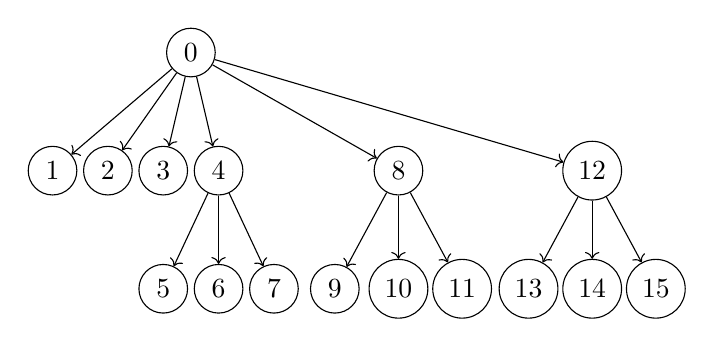
\begin{tikzpicture} [every node/.style = {shape=circle, draw, align=center}]
        % \tikzstyle{level 1}=[sibling distance=4em]
        % \tikzstyle{level 2}=[sibling distance=2em]
        \node {0}
        child [->, sibling distance=2em] { node {1}}
        child [->, sibling distance=2em] { node {2}}
        child [->, sibling distance=2em] { node {3}}
        child  [->, sibling distance=2em] { node {4}
            child [sibling distance=2em] {node {5}}
            child [sibling distance=2em] {node {6}}
            child [sibling distance=2em] {node {7}}
        }
        child [->, sibling distance=5em] { node {8}
            child [sibling distance=2.3em] {node {9}}
            child [sibling distance=2.3em] {node {10}}
            child [sibling distance=2.3em] {node {11}}
        }
        child [->, sibling distance=5.8em] { node {12}
            child [sibling distance=2.3em] {node {13}}
            child [sibling distance=2.3em] {node {14}}
            child [sibling distance=2.3em] {node {15}}
        };


    \end{tikzpicture}
    \caption{4-nomial broadcast with 16 processes.}
    \label{fig:graph-knomial}
\end{figure}
% \lstset{label = lst:topo-knomial}
% \lstset{caption = Heuristic for rank reordering knomial trees.}
% \lstinputlisting[float=!htbp]{3_Chapters/4_Chapter_TopologyAwareness/Figures/Topo_Knomial.c}
\begin{algorithm}
  \caption{Knomial Heuristic}
  \label{alg:knomial}
  \begin{algorithmic}[1]
    \Require Number of Processes p, physical topology distance matrix D, knomial fan-out k
    \Ensure  Mapping array M representing the new rank for each process

    \State M[0] = 0;
    \State REC\_KNOM\_MAP(0, p)

    \Procedure{rec\_knom\_map}{ref\_rank, upper\_lim}
    \For{\textit{i from ref\_rank + 1 to ref\_rank + k - 1}}
    \State M[i] = find\_closest\_to(ref\_rank, D);
    \EndFor
    \State mask = 1
    \While{\textit{(mask*k) $<$ upper\_lim}}
    \For{\textit{i from 1 to k}}
    \State new\_rank = ref\_rank + (mask * k * i)
    \If {\textit{new\_rank $\geq$ upper\_lim}}
    \State \textbf{break};
    \EndIf
    \State M[new\_rank] = closest\_core(ref\_rank, D);
    \State new\_lim = ref\_rank + k * mask
    \State REC\_KNOM\_MAP(new\_rank, new\_lim)
    \EndFor
    \State mask *= k
    \EndWhile
    \EndProcedure

  \end{algorithmic}
\end{algorithm}

\subsection{Hessam's work on Binomial, Ring, and Recursive Doubling}

Previous work by Mirsadeghi and Afsahi \cite{Mirsadeghi2016TopoAwareCollRR} proposed a series of algorithms targeting recursive doubling allgather, ring, binomial broadcast, and binomial gather. 
While their work is evaluated in the context of allgather, the reordering heuristics they propose can also be used to accelerate allreduce. 

The ring and recursive doubling allgather heuristics can be transplanted directly to ring and recursive doubling allreduce, respectively, and the intuition behind both algorithm's utilities generally holds. 
The ring targets nearest neighbour ranks, it starts at rank 0 and walks through the communicator mapping $r+1$ as close as possible to reference rank $r$, then setting $r+1$ as the new reference rank.
Since both ring allreduce and ring allgather only communicate with immediate neighbours (i.e. rank $r+1$ and $r-1$), the intuition of this heuristic is portable across collectives.
The recursive doubling algorithm targets the last two stages of the algorithm, as message sizes are the largest during those phases. 
It's similar to our proposed RSA heuristic but focuses on the last rounds of communication instead of the first. 
Recursive doubling allreduce and allgather share the same communication pattern, but while the message sizes double each round in allgather,  it remains fixed in allreduce.
So migrating the heuristic to allreduce might not see the same performance gains, but it will ensure that most communications take an efficient path.

We also evaluated the previously proposed recursive doubling allgather heuristic in the context of the scatter-allgather broadcast.
Scatter-allgather, also known as Van de Geijn's algorithm, is often used for large message broadcasts as it is incredibly bandwidth efficient, 
This is achieved by splitting the message up into segments, scattering the segments across the communicator with a binomial algorithm, and then reconstructing the message with an allgather of the segments.
The recursive doubling allgather has already been studied in \cite{Mirsadeghi2016TopoAwareCollRR}, it has an even communication pattern where the last stages of the algorithm have the largest message sizes.
On the other hand, the binomial scatter is similar to the binomial broadcast algorithm, with the difference that the message size halves between stages. 
The communication graph generated by the binomial pattern is essentially a subgraph of recursive doubling, so it can be layered on top of recursive doubling without adding any new communication dependencies. 
Therefore, we applied the recursive doubling reordering heuristic to scatter allgather broadcasts.

\section{Experiments and Analysis}
To evaluate our new heuristics, as well as the previously proposed heuristics, we orchestrated everything into OpenMPI.
We compare our heuristics against SCOTCH, a commonly used graph partitioning library previously applied to topology-aware works.
Through microbenchmark evaluation, we are able to demonstrate that our method can improve allreduce performance, depending on the initial mapping.

\subsection{Software Implementation}
We implemented our method within OpenMPI v4.0.5 \cite{gabriel2004OpenMPI}.
Building on top of OpenMPI let us leverage the existing collective implementations as well as the algorithm selection mechanism.
OpenMPI also has support for Hwloc integrated within the runtime, making topology detection easier.

There are some caveats with collective rank reordering as not all collectives can support it seamlessly.
By default, MPI\_Allreduce algorithms assume operations are commutative, but a user can specify an operation to be non-commutative with respect to process's ranks. 
To support non-commutative operations, Allreduce algorithms must be carefully designed to ensure operations are applied in the correct order, but renumbering processes break that careful design.
Therefore, this work only supports commutative operations.
Furthermore, both broadcast heuristics assume rank 0 is the root which is not always true. 
So when rank 0 isn't the broadcast root, it needs to receive the data from the real root before it can start the broadcast on the shadow-communicator.
In retrospect, a smarter design would have been to assign virtual ranks by shifting each rank according to the root's value, this would make the root 0.
But I last looked at the code for remapping a year ago, and the performance difference provided by this step would be negligible; furthermore, OMB only calls bcast w/ root 0, and Horovod doesn't use bcast.

We leverage existing system topology detection tools to generate the host topology matrix.
Hwloc \cite{Broquedis2010hwloc} is a tool for gathering intranode topology information, this includes NUMA domains and cache hierarchies.
To extract the network topology, we started by collecting topology information using cluster-provided tools, ibnetdiscovee for Beluga's InfiniBand network and Opareport for Cedar's OmniPath fabric.
We then transformed both files into a common format and saved them to disk.
When creating a topology matrix, each node is responsible for generating the row corresponding to its rank, this is done by indexing to the topology file and checking neighbouring ranks with Hwloc, then an allgather is performed to combine all processes' node information and generate the final results.
This method can require is not scalable as the memory requirements are on the order of $O(n^2)$ with respect to the number of processes, but it is viable for the scale we're running at.

OpenMPI does support CUDA memory transfers, but their implementation is not efficient. 
When allreduce is called on GPU memory, the data is copied to a temporary host buffer, then a CPU-based allreudce is performed and the final result is copied back up to the GPU.
While this does fulfill the MPI specification, it neglects to use the available GPU hardware like compute kernel reduction or GPU to GPU data transfers with NVLinks.
So we modified OpenMPI's RSA algorithm to make use of GPU hardware, this is also more in line with how modern collective libraries like NCCL and UCC implement allreduce \cite{UCC, NCCL}.

To compare our proposed heuristics against an established topology mapping tool, we also integrated the SCOTCH graph embedding tool \cite{Pellegrini2012SCOTCH} into the rank reordering method.
SCOTCH uses a graph bisecting method to perform graph partitioning and embedding, and it has been used in previous work to incorporate topology awareness \cite{Mirsadeghi2016TopoAwareCollRR}.

The rank reordering strategy finds performance improvements by rearranging the process to core bindings, which implies that any performance improvements are dependent on the initial process to core bindings.
MPI implementations provide flags for users to specify how processes should be distributed at job launch. 
While not exhaustive, this interface does provide a starting point for users to optimize the process to node mappings.
Our method can calculate more complicated mappings, as well as mappings for subsets of processes for when an application uses subcommunicators.  

In OpenMPI, users can specify a resource and processes are bound to that resource in a round-robin fashion.
Figure \ref{fig:init-mappings} provides an example outlining the three initial mappings we evaluated.
The default initial mapping is by-package, this takes a node and fills it with processes alternating between packages until the node is full, it then repeats this on the next node until all processes are bound.
By-core mapping places processes to consecutively numbered cores filling up a node before moving to the next, and by-node scatters processes across nodes by cycling through nodes and placing processes one at a time.

\begin{figure}
  \centering
  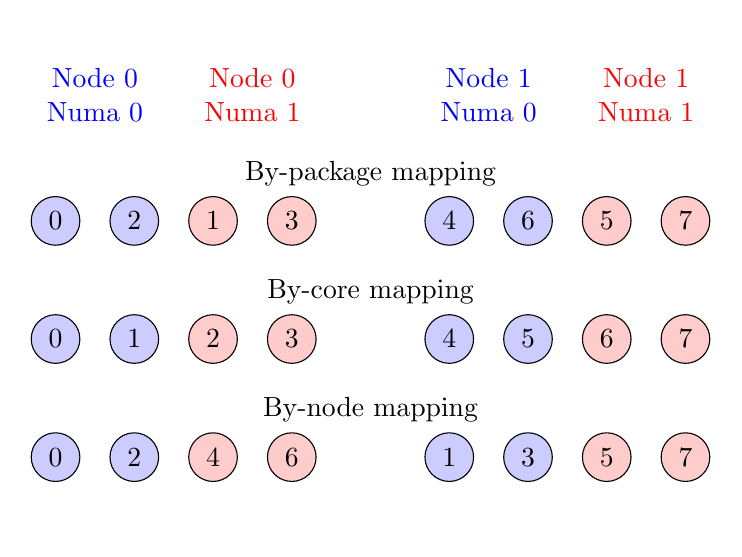
\begin{tikzpicture}[every node/.style = {shape=circle, draw, align=center}]
    \node at (0.5, 4.6) [draw=none, text=blue] {Node 0\\Numa 0};
    \node at (2.5, 4.6) [draw=none, text=red] {Node 0\\Numa 1};
    \node at (5.5, 4.6) [draw=none, text=blue] {Node 1\\Numa 0};
    \node at (7.5, 4.6) [draw=none, text=red] {Node 1\\Numa 1};
  
    \node at (0, 3) [fill=blue!20] {0};
    \node at (1, 3) [fill=blue!20] {2};
    \node at (2, 3) [fill=red!20] {1};
    \node at (3, 3) [fill=red!20] {3};
    \node at (4, 3.6) [draw=none] {By-package mapping};
    \node at (5, 3) [fill=blue!20] {4};
    \node at (6, 3) [fill=blue!20] {6};
    \node at (7, 3) [fill=red!20] {5};
    \node at (8, 3) [fill=red!20] {7};
    
    \node at (0, 1.5) [fill=blue!20] {0};
    \node at (1, 1.5) [fill=blue!20] {1};
    \node at (2, 1.5) [fill=red!20] {2};
    \node at (3, 1.5) [fill=red!20] {3};
    \node at (4, 2.1) [draw=none] {By-core mapping};
    \node at (5, 1.5) [fill=blue!20] {4};
    \node at (6, 1.5) [fill=blue!20] {5};
    \node at (7, 1.5) [fill=red!20] {6};
    \node at (8, 1.5) [fill=red!20] {7};

    \node at (0, 0) [fill=blue!20] {0};
    \node at (1, 0) [fill=blue!20] {2};
    \node at (2, 0) [fill=red!20] {4};
    \node at (3, 0) [fill=red!20] {6};
    \node at (4, 0.6) [draw=none] {By-node mapping};
    \node at (5, 0) [fill=blue!20] {1};
    \node at (6, 0) [fill=blue!20] {3};
    \node at (7, 0) [fill=red!20] {5};
    \node at (8, 0) [fill=red!20] {7};
  \end{tikzpicture}
  \caption[OpenMPI Process to core binding options]{
      Example of by-package, by-core and by-node initial mappings on 2 nodes with 2 2-core processors per node. 
      The blue dots represent package 0, and the red dots represent package 1.
  }
  \label{fig:init-mappings}
\end{figure}

\subsection{Hardware}\label{sec:topo-eval-hardware}
% We evaluated our work on two heterogeneous clusters, Beluga and Cedar, provided by Compute Canada. 
% Beluga is Infiniband based, structured as a 5:1 blocking fat tree with static routing.  
% The CPU nodes have dual socket Xeon Gold 6148 Skylake processors, and the GPU nodes use the same processors attached to 4 V100s fully connected with NVLink.
% Cedar, on the other hand, is OmniPath based.
% It also has a fat-tree topology configured, bus it is configured with 2:1 blocking and has adaptive routing.
% Cedar's CPU allocation has dual-socket 24-core Xeon Platinum 8260 Cascade Lake processors, while the GPU nodes have two 20-core Xeon Silver 4216 Cascade Lake processors hosting four v100s GPUs interconnected by NVLink.

We evaluated our work on Beluga, a heterogeneous cluster hosted by Polytechnique Montréal and with access provided by Compute Canada. 
Beluga is an Infiniband based cluster, structured with a 5:1 blocking fat tree with static routing.
The CPU nodes have dual socket Xeon Gold 6148 Skylake processors, and the GPU nodes use the same processors attached to 4 V100s fully connected with NVLink.

\subsection{Results}

% \begin{figure*}
    \centering
    \begin{tikzpicture}
        \begin{groupplot}[group style={
                        group size=2 by 3,
                        xlabels at=edge bottom,
                        ylabels at=edge left,
                        xticklabels at=edge bottom,
                        yticklabels at=edge left,
                        vertical sep=1.5cm,
                    },
                height=5.7cm,
                width=7.5cm,
                xlabel={Message Size (Bytes)},
                ylabel={Fractional Improvement},
                legend style={at={(-0.1,-0.3)}, anchor=north},
                legend columns=3,
                ymin = -0.5,
                ymax = 1,
                xmin = 1,
                xmax = 1073741824,
                grid=both,
            ]
            \nextgroupplot[xmode=log, title=GPU By Socket]
            \addplot table[x=msize, y=rsa_dif] {3_Chapters/4_Chapter_TopologyAwareness/Figures/data/beluga/ar/bysoc_gpu_2.dat};
            \addplot table[x=msize, y=ring_dif] {3_Chapters/4_Chapter_TopologyAwareness/Figures/data/beluga/ar/bysoc_gpu_2.dat};
            \addplot table[x=msize, y=rdouble_dif] {3_Chapters/4_Chapter_TopologyAwareness/Figures/data/beluga/ar/bysoc_gpu_2.dat};
            
            \nextgroupplot[xmode=log, title=CPU By Socket]
            \addplot table[x=msize, y=rsa_pdif] {3_Chapters/4_Chapter_TopologyAwareness/Figures/data/beluga/ar/bysoc_cpu_2.dat};
            \addplot table[x=msize, y=ring_pdif] {3_Chapters/4_Chapter_TopologyAwareness/Figures/data/beluga/ar/bysoc_cpu_2.dat};
            \addplot table[x=msize, y=rdouble_pdif] {3_Chapters/4_Chapter_TopologyAwareness/Figures/data/beluga/ar/bysoc_cpu_2.dat};
            
            \nextgroupplot[xmode=log, title=GPU By Core]
            \addplot table[x=msize, y=rsa_dif] {3_Chapters/4_Chapter_TopologyAwareness/Figures/data/beluga/ar/bycore_gpu_2.dat};
            \addplot table[x=msize, y=ring_dif] {3_Chapters/4_Chapter_TopologyAwareness/Figures/data/beluga/ar/bycore_gpu_2.dat};
            \addplot table[x=msize, y=rdouble_dif] {3_Chapters/4_Chapter_TopologyAwareness/Figures/data/beluga/ar/bycore_gpu_2.dat};
            
            \nextgroupplot[xmode=log, title=CPU By Core, legend]
            \addplot table[x=msize, y=rsa_pdif] {3_Chapters/4_Chapter_TopologyAwareness/Figures/data/beluga/ar/bycore_cpu_2.dat};
            \addplot table[x=msize, y=ring_pdif] {3_Chapters/4_Chapter_TopologyAwareness/Figures/data/beluga/ar/bycore_cpu_2.dat};
            \addplot table[x=msize, y=rdouble_pdif] {3_Chapters/4_Chapter_TopologyAwareness/Figures/data/beluga/ar/bycore_cpu_2.dat};
            
            \nextgroupplot[xmode=log, title=GPU By Node, xticklabels={8B, 1kB, 64kB, 8MB}]
            \addplot table[x=msize, y=rsa_dif] {3_Chapters/4_Chapter_TopologyAwareness/Figures/data/beluga/ar/bynode_gpu_2.dat};
            \addplot table[x=msize, y=ring_dif] {3_Chapters/4_Chapter_TopologyAwareness/Figures/data/beluga/ar/bynode_gpu_2.dat};
            \addplot table[x=msize, y=rdouble_dif] {3_Chapters/4_Chapter_TopologyAwareness/Figures/data/beluga/ar/bynode_gpu_2.dat};
            
            
            \nextgroupplot[xmode=log, title=CPU By Node, xticklabels={8B, 1kB, 64kB, 8MB}]
            \addplot table[x=msize, y=rsa_pdif] {3_Chapters/4_Chapter_TopologyAwareness/Figures/data/beluga/ar/bynode_cpu_2.dat};
            \addplot table[x=msize, y=ring_pdif] {3_Chapters/4_Chapter_TopologyAwareness/Figures/data/beluga/ar/bynode_cpu_2.dat};
            \addplot table[x=msize, y=rdouble_pdif] {3_Chapters/4_Chapter_TopologyAwareness/Figures/data/beluga/ar/bynode_cpu_2.dat};
            
            \addlegendentry{RSA}
            \addlegendentry{Ring}
            \addlegendentry{Recursive Doubling}
            
        \end{groupplot}
    \end{tikzpicture}
    \caption{Fractional improvement of Allreduce heuristics on Beluga.
    CPU and GPU were evaluated with by-socket, by-core and by-node initial mappings.
    Messages varry from 4B to 128MB.}
    \label{fig:beluga-ar-frac-imprv}
\end{figure*}


% \begin{figure*}
    \centering
    \begin{tikzpicture}
        \begin{groupplot}[group style={
                        group size=2 by 3,
                        xlabels at=edge bottom,
                        ylabels at=edge left,
                        xticklabels at=edge bottom,
                        yticklabels at=edge left,
                        vertical sep=1.5cm,
                    },
                height=5.7cm,
                width=7.5cm,
                xlabel={Message Size (Bytes)},
                ylabel={Fractional Improvement},
                legend style={at={(-0.1,-0.3)}, anchor=north},
                legend columns=3,
                ymin = -0.5,
                ymax = 1,
                xmin = 1,
                xmax = 1073741824,
                grid=both,
            ]
            \nextgroupplot[xmode=log, title=GPU By Socket]
            \addplot table[x=msize, y=k_dif] {3_Chapters/4_Chapter_TopologyAwareness/Figures/data/beluga/bc/bysoc_gpu.dat};
            \addplot table[x=msize, y=bin_dif] {3_Chapters/4_Chapter_TopologyAwareness/Figures/data/beluga/bc/bysoc_gpu.dat};
            \addplot table[x=msize, y=scag_dif] {3_Chapters/4_Chapter_TopologyAwareness/Figures/data/beluga/bc/bysoc_gpu.dat};
            
            \nextgroupplot[xmode=log, title=CPU By Socket]
            \addplot table[x=msize, y=k_dif] {3_Chapters/4_Chapter_TopologyAwareness/Figures/data/beluga/bc/bysoc_cpu.dat};
            \addplot table[x=msize, y=bin_dif] {3_Chapters/4_Chapter_TopologyAwareness/Figures/data/beluga/bc/bysoc_cpu.dat};
            \addplot table[x=msize, y=scag_dif] {3_Chapters/4_Chapter_TopologyAwareness/Figures/data/beluga/bc/bysoc_cpu.dat};
            
            \nextgroupplot[xmode=log, title=GPU By Core]
            \addplot table[x=msize, y=k_dif] {3_Chapters/4_Chapter_TopologyAwareness/Figures/data/beluga/bc/bycore_gpu.dat};
            \addplot table[x=msize, y=bin_dif] {3_Chapters/4_Chapter_TopologyAwareness/Figures/data/beluga/bc/bycore_gpu.dat};
            \addplot table[x=msize, y=scag_dif] {3_Chapters/4_Chapter_TopologyAwareness/Figures/data/beluga/bc/bycore_gpu.dat};
            
            \nextgroupplot[xmode=log, title=CPU By Core, legend]
            \addplot table[x=msize, y=k_dif] {3_Chapters/4_Chapter_TopologyAwareness/Figures/data/beluga/bc/bycore_cpu.dat};
            \addplot table[x=msize, y=bin_dif] {3_Chapters/4_Chapter_TopologyAwareness/Figures/data/beluga/bc/bycore_cpu.dat};
            \addplot table[x=msize, y=scag_dif] {3_Chapters/4_Chapter_TopologyAwareness/Figures/data/beluga/bc/bycore_cpu.dat};
            
            \nextgroupplot[xmode=log, title=GPU By Node, xticklabels={8B, 1kB, 64kB, 8MB}]
            \addplot table[x=msize, y=k_dif] {3_Chapters/4_Chapter_TopologyAwareness/Figures/data/beluga/bc/bynode_gpu.dat};
            \addplot table[x=msize, y=bin_dif] {3_Chapters/4_Chapter_TopologyAwareness/Figures/data/beluga/bc/bynode_gpu.dat};
            \addplot table[x=msize, y=scag_dif] {3_Chapters/4_Chapter_TopologyAwareness/Figures/data/beluga/bc/bynode_gpu.dat};
            
            
            \nextgroupplot[xmode=log, title=CPU By Node, xticklabels={8B, 1kB, 64kB, 8MB}]
            \addplot table[x=msize, y=k_dif] {3_Chapters/4_Chapter_TopologyAwareness/Figures/data/beluga/bc/bynode_cpu.dat};
            \addplot table[x=msize, y=bin_dif] {3_Chapters/4_Chapter_TopologyAwareness/Figures/data/beluga/bc/bynode_cpu.dat};
            \addplot table[x=msize, y=scag_dif] {3_Chapters/4_Chapter_TopologyAwareness/Figures/data/beluga/bc/bynode_cpu.dat};
            
            \addlegendentry{Knomial}
            \addlegendentry{Bin-Tree}
            \addlegendentry{SCAG}
        \end{groupplot}
    \end{tikzpicture}
    \caption{Fractional improvement of Broadcast heuristics on Beluga. 
    CPU and GPU were evaluated with by-socket, by-core and by-node initial mappings.
    Messages varry from 1B to 128MB.}
    \label{fig:beluga-bc-frac-imprv}
\end{figure*}

% \begin{figure*}
    \centering
    \begin{tikzpicture}
        \begin{groupplot}[group style={
                        group size=2 by 3,
                        xlabels at=edge bottom,
                        ylabels at=edge left,
                        xticklabels at=edge bottom,
                        yticklabels at=edge left,
                        vertical sep=1.3cm,
                    },
                height=5.7cm,
                width=7.5cm,
                xlabel={Message Size (Bytes)},
                ylabel={Speedup},
                legend style={at={(-0.2, -0.3)}, anchor=north},
                legend columns=4,
                ymin = -1,
                ymax = 1,
                xmin = 1,
                xmax = 1073741824,
                grid=both,
            ]

            \nextgroupplot[xmode=log, title=GPU By Socket]
            \addplot[blue, mark=*] table[x=msize, y=tt_pdif] {3_Chapters/4_Chapter_TopologyAwareness/Figures/data/beluga/mandm/data/ar_gpu_bysoc_64.dat};
            \addplot[dashed, blue, mark=star] table[x=msize, y=s_pdif] {3_Chapters/4_Chapter_TopologyAwareness/Figures/data/beluga/mandm/data/ar_gpu_bysoc_64.dat};
            \addplot[red, mark=*] table[x=msize, y=tt_pdif] {3_Chapters/4_Chapter_TopologyAwareness/Figures/data/beluga/mandm/data/bc_gpu_bysoc_64.dat};
            \addplot[dashed, red, mark=star] table[x=msize, y=s_pdif] {3_Chapters/4_Chapter_TopologyAwareness/Figures/data/beluga/mandm/data/bc_gpu_bysoc_64.dat};

            \nextgroupplot[xmode=log, title=CPU By Socket]
            \addplot[blue, mark=*] table[x=msize, y=remap_pdif] {3_Chapters/4_Chapter_TopologyAwareness/Figures/data/beluga/mandm/data/cpu/ar_bysoc.dat};
            \addplot[blue, mark=star] table[x=msize, y=scotch_pdif] {3_Chapters/4_Chapter_TopologyAwareness/Figures/data/beluga/mandm/data/cpu/ar_bysoc.dat};
            \addplot[red, mark=*] table[x=msize, y=remap_pdif] {3_Chapters/4_Chapter_TopologyAwareness/Figures/data/beluga/mandm/data/cpu/bc_bysoc.dat};
            \addplot[red, mark=star] table[x=msize, y=scotch_pdif] {3_Chapters/4_Chapter_TopologyAwareness/Figures/data/beluga/mandm/data/cpu/bc_bysoc.dat};

            \nextgroupplot[xmode=log, title=GPU By Core]
            \addplot[blue, mark=*] table[x=msize, y=tt_pdif] {3_Chapters/4_Chapter_TopologyAwareness/Figures/data/beluga/mandm/data/ar_gpu_bycore_64.dat};
            \addplot[dashed, blue, mark=star] table[x=msize, y=s_pdif] {3_Chapters/4_Chapter_TopologyAwareness/Figures/data/beluga/mandm/data/ar_gpu_bycore_64.dat};
            \addplot[red, mark=*] table[x=msize, y=tt_pdif] {3_Chapters/4_Chapter_TopologyAwareness/Figures/data/beluga/mandm/data/bc_gpu_bycore_64.dat};
            \addplot[dashed, red, mark=star] table[x=msize, y=s_pdif] {3_Chapters/4_Chapter_TopologyAwareness/Figures/data/beluga/mandm/data/bc_gpu_bycore_64.dat};
            
            \nextgroupplot[xmode=log, title=CPU By Core]
            \addplot[blue, mark=*] table[x=msize, y=remap_pdif] {3_Chapters/4_Chapter_TopologyAwareness/Figures/data/beluga/mandm/data/cpu/ar_bycore.dat};
            \addplot[blue, mark=star] table[x=msize, y=scotch_pdif] {3_Chapters/4_Chapter_TopologyAwareness/Figures/data/beluga/mandm/data/cpu/ar_bycore.dat};
            \addplot[red, mark=*] table[x=msize, y=remap_pdif] {3_Chapters/4_Chapter_TopologyAwareness/Figures/data/beluga/mandm/data/cpu/bc_bycore.dat};
            \addplot[red, mark=star] table[x=msize, y=scotch_pdif] {3_Chapters/4_Chapter_TopologyAwareness/Figures/data/beluga/mandm/data/cpu/bc_bycore.dat};
            
            \nextgroupplot[xmode=log, title=GPU By Node, xticklabels={1B, 10kB, 100kB, 10MB, 1GB}]
            \addplot[blue, mark=*] table[x=msize, y=tt_pdif] {3_Chapters/4_Chapter_TopologyAwareness/Figures/data/beluga/mandm/data/ar_gpu_bynode_64.dat};
            \addplot[dashed, blue, mark=star] table[x=msize, y=s_pdif] {3_Chapters/4_Chapter_TopologyAwareness/Figures/data/beluga/mandm/data/ar_gpu_bynode_64.dat};
            \addplot[red, mark=*] table[x=msize, y=tt_pdif] {3_Chapters/4_Chapter_TopologyAwareness/Figures/data/beluga/mandm/data/bc_gpu_bynode_64.dat};
            \addplot[dashed, red, mark=star] table[x=msize, y=s_pdif] {3_Chapters/4_Chapter_TopologyAwareness/Figures/data/beluga/mandm/data/bc_gpu_bynode_64.dat};

            \nextgroupplot[xmode=log, title=CPU By Node, xticklabels={1B, 10kB, 100kB, 10MB, 1GB}]
            \addplot[blue, mark=*] table[x=msize, y=remap_pdif] {3_Chapters/4_Chapter_TopologyAwareness/Figures/data/beluga/mandm/data/cpu/ar_bynode.dat};
            \addplot[blue, mark=star] table[x=msize, y=scotch_pdif] {3_Chapters/4_Chapter_TopologyAwareness/Figures/data/beluga/mandm/data/cpu/ar_bynode.dat};
            \addplot[red, mark=*] table[x=msize, y=remap_pdif] {3_Chapters/4_Chapter_TopologyAwareness/Figures/data/beluga/mandm/data/cpu/bc_bynode.dat};
            \addplot[red, mark=star] table[x=msize, y=scotch_pdif] {3_Chapters/4_Chapter_TopologyAwareness/Figures/data/beluga/mandm/data/cpu/bc_bynode.dat};
            
            \addlegendentry{Allreduce remap}
            \addlegendentry{Allreduce SCOTCH}
            \addlegendentry{Bcast remap}
            \addlegendentry{Bcast SCOTCH}

        \end{groupplot}
    \end{tikzpicture}
    \caption{Perforamce improvement over out-of-the-box OpenMPI on 16 GPU nodes, and 32 CPU nodes. 
    Red lines are MPI\_Allreduce, blue lines are MPI\_Bcast.
    Solid lines are reordered with proposed heuristics, and dashed lines are reordered with scotch.
    }
    \label{fig:beluga-mandm-dual-64-1024}
\end{figure*}


We used OSU-Microbenchamrks v5.7 \cite{Bureddy2012OMB} to evaluate the performance of our proposed method. 
This tool performs 1000 loops over MPI\_Allreduce, measures the runtime of each function call, and outputs the average latency. 
It also provides the option to locate the data buffer in either CPU memory or GPU memory.

Figure \ref{fig:beluga-ar-frac-imprv} demonstrates allreduce's rank reordering for both CPU and GPU nodes.
GPU jobs were evaluated with 16 nodes (64 GPUs total), while CPU jobs were run across 32 nodes with 32 processes per node (1024 ranks total).
The ring and RSA algorithms show ideal performance in that they're often on-par or better than the initial mapping, save for a few outliers.
This shows how the proposed heuristics find a near-ideal mapping or at least a mapping equivalent to the initial conditions.

One immediately obvious observation is that any improvements are more pronounced on CPUs compared to GPUs, but this can be explained by the amount of contention on underlying resources.
When using CPUs, any cross-socket communication needs to traverse the QPI link, which can easily become a bottleneck when multiple processes try to concurrently send large messages across it.
Take RSA applied to a by-package initial mapping as an example.
The by-package initial mapping places consecutive ranks on different nodes, forcing all the largest messages to traverse the QPI link. 
If 32 ranks perform a 64MB allreduce, that would generate 512MB of unidirectional contention across 16 ranks during the first stage.
The reordering moves all these large message transfers to within the same socket, removing the QPI bottleneck and gaining 10\% performance improvement.   
Further, the ring algorithm sees even more improvement with a by-socket mapping since each rank has to send every message to a different NUMA region.
By moving as many messages as possible within the same socket, the ring heuristic can find near 50\% performance improvement.
% The best example for this would be a ring algorithm with a by-package initial mapping.
% With a by-package mapping, consecutive ranks are placed on different sockets, and since communications in ring only happen between consecutive ranks, all intranode communication needs to traverse the QPI.
% Reordering fixes this by rearranging consecutive ranks to be as close as possible, leading to only one message needing to traverse the QPI link, removing QPI contention and providing up to 50\% performance improvements. 
But, GPUs don't generate the same contention since there are only four processes per node, so the resource demand is much smaller.
Further, the GPUs are fully connected with NVLINK intranode, so there is no single link bottleneck.
This hardware difference leads to the same reordering heuristics generating no performance differences when using GPUs.

The next thing to note would be how the most dramatic performance improvements are seen on the by-node mapping, specifically for ring and RSA. 
The by-node initial mapping places the most intense communications of the RSA algorithm on inter-node links, and literally, all communication in the ring algorithm is forced over the network.
The reordering results in massive performance improvements by moving large chunks of communication internode and provides up to 80\% improvement for ring and RSA on CPUs.
This large performance improvement is justified as the Infiniband link is the lowest bandwidth component in the system, as well as there only being one NIC having to service all 4/32 processes per node.

In retrospect, using recursive doubling is dumb, it produces mappings where one process per node has the bulk of its partners on the same node, but the rest of the processes need to exchange their data off the node. 
It's hard to notice with small communicator sizes, but when you scale it up so that $numnodes > processes per node$, it becomes more evident.
But at the same time, I should have seen the negative performance when I was developing this trash and gone, "\textit{That's weird, I should investigate why that deteriorates...}".
Now I feel like a complete idiot for proposing this idea, should scrap it and pretend it never happened?

The results for the evaluated broadcast remappings are presented in figure \ref{fig:beluga-bc-frac-imprv}.
The broadcast algorithms see substantial improvements across the board. 
Many of the same characteristics map to the broadcast remappings, CPU results are much more dramatic than GPU results as there is more resource contention, and improvements are also greater when communication can be pulled off the network. 
The most obvious example of saving network resources would be the by-node knomial broadcast, as this moves all child communications from off-rank to within the same node, where they can leverage more efficient shared memory communications. 
Another example of saving network resources is the binary tree broadcast.
The by-package and by-core mappings see between 50\% to 80\% performance improvements across both GPU and CPU allocations, but near 0 improvements for by-node, this outlines how OpenMPI's binary tree implementation drives most of the communication to the network for core/socket initial mappings. 

Scatter allgather is an interesting case, as it can see strong improvements for by-core and by-package initial mappings, showing how moving the large transfers in binomial scatter can save time. 
Interestingly though, it loses performance on a by-node mapping, so clearly, there is performance left on the table, and more work could be done.

To compare our work against other graph reordering tools, we integrated SCOTCH \cite{Pellegrini2012SCOTCH} into our method and show its performance results in figure \ref{fig:beluga-mandm-dual-64-1024}.
Once again, we ran with 16 GPU nodes and 32 CPU nodes, but this time we used OpenMPI's tuning table to select which algorithm to use based on its tuning table.
Each heuristic provides a more efficient mapping than anything SCOTCH can generate, as is evidenced by the superior performance. 
That said, OpenMPI's algorithm selection works efficiently out-of-the-box for both by-core and by-node mappings, but we are able to provide improvements when using a by-node mapping.  

\section{I can't believe it's not a conclusion ™}
This chapter expands on the work proposed by Mirsadeghi and Afsahi \cite{Mirsadeghi2016TopoAwareCollRR} by expanding their idea to new collective communication algorithms.
We show that their methods can viably be applied to RSA, ring, and recursive doubling allreduce, along with binary-tree, knomial, and scatter-allgather broadcast.
Depending on the initial mapping, we can see performance improvements in the range of 10\% to 80\%.
While this work is best applied to dense CPU allocations, it can be applied to GPU allocations as well. 

The idea of this work was to accelerate allreduce through the topology-aware algorithms, with the motivation of decreaseing deep learning training time.
Topology awareness has been exhaustively evaluated by many researchers, with a plethora of ideas existing in the literature.
But, topology awareness is not the only strategy for accelerating allreduce.
In the next chapter, we tackle the same problem of accelerating allreduce but from the angle of process arrival pattern awareness.
This is still in the domain of large-message allreudce so many existing algorithms are applicable, but there are numerus differences and new challenges which require clever and innovative ideas to solve.

% Conseptualy, this problem can be treated as a graph mapping problem. 
% The MPI application is modeld as weighted graph $G=(V_G, w_G)$, where verticeis are processes and weights are the amount of communication between processes.
% The host topology is also models as a weighted graph $H=(V_h, w_H)$, where vertices are processing elements and weights represent the capacity of the interconnect between any two processing elements.
% % $G$ and $H$ are both fully connected graphs, and $|V_G| = |V_H|$.
% When running the application, the grpah $G$ is mapped to $H$ so that each rank in $V_G$ is overlayed on a processing element in $V_H$, and communication weights in $w_G$ are tied to a hardware link $w_H$.
% Lastly, a mathematical metric is defined to estimate the performance of the mapping.
% So the goal of topology-awareness is to find a mapping from $G$ to $H$ that minimized/maximized a defined metric.
% This problem, which is a subset of graph-embedding, is NP-hard, so finding optimal solutions for large scale instances of this problem is not feasable \cite{Hoefler2011GenericTopoMappingStrats}.
% Solutions used in practice often rely on heuristics to find near-optimal solutions in a reasonable amount of time.
% Chapter 5 - Process Arrival Pattern Awareness

% \glsresetall % reset the glossary to expand acronyms again
\chapter[Process Arrival Pattern Awareness]{Process Arrival Pattern Awareness}\label{ch:PAPAwareness}
\index{Process Arrival Pattern Awareness}

\begin{itemize}
    \item Background on Process Arrival Pattern Awareness
    \begin{itemize}
        \item Pedram's characterization work, mention that Horovod can see PAP imbalacen in range of 2-6, \cite{Alizadeh2022PAPCollDL, Mohammadalizadehbakhtevari2021Thesis}
        \item Maximum/Average Imbalance Factor and EQs
    \end{itemize}
    \item Methods
    \item Evaluation
    \begin{itemize}
        \item Horovod? Cos  moflow?
    \end{itemize}
\end{itemize}

\section{Motivation}

This chapter approaches allreduce collective design through the lens of process arrival pattern (PAP) awareness. 
When designing collective algorithms, developers often assume that all processes arrive at the same time, but this is not a safe assumption.
The order and timing that processes enter the collective can have an impact on the algorithm's performance, and this work tries to leverage the arrival imbalance to improve the overall collective performance.
Deep learning is a difficult application to load balance due to the stochastic nature of datasets, leading to increased arrival imbalance at collectives \cite{Mohammadalizadehbakhtevari2021Thesis, Alizadeh2022PAPCollDL, Li2020DLPartialColl}. 
While PAP-aware collective algorithms do exist, no existing algorithms target multi-node GPU deployments, so to fill this gap, we propose a UCX-RMA-based PAP distribution mechanism with an accompanying allreduce algorithm which shows \_\% improvement over default allreduce algorithms performance under arrival imbalance.  

There are previously proposed methods and algorithms that leverage PAP awareness to accelerate collectives, this chapter starts by surveying existing work.
We outline some analysis on how PAP affects collectives, outlining our approach to accelerate allreduce.
The main contribution is a novel cluster-wide method of sharing PAP information with an accompanying allreduce algorithm designed to perform better than existing algorithms under a processes arrival imbalance.
We evaluate our work using an imbalance factor-inducing benchmark and show that we can see \_\% improvement over state-of-the-art algorithms.  


\subsection{Related Work}
Mamidala et al. \cite{Mamidala2004BarrierAllreduceIBAdaptive} propose a PAP-Aware tree-based algorithm that can be applied to barrier and allreduce collectives.
Their method involves rebalancing a k-ary tree by passing a token between ranks.
For the process holding the token, when $k-1$ child processes have arrived, the token is passed to the $k^{th}$ child through an RDMA write.
If an arriving process is holding the token and all its child processes have arrived, it knows it's the last to arrive, so it triggers a multicast releasing all ranks from the barrier. 

Faraj et al. \cite{Faraj2008StudyProcArrivalMPIColl} evaluate process arrival imbalance at collectives across a handful of MPI kernels.
The PMPI profiling interface was used to introspect the kernel runtime and collect PAP statistics on two different clusters.
The authors determine that process imbalance is unavoidable; even if the workload is perfectly balanced at the application level, the complexity of these massive systems will inevitably lead to differences in arrival time. 
But, regular imbalance patterns do emerge during application runtime, and specific collective call sites will exhibit the same imbalance multiple times during execution.
They also measure the effect of process imbalance on specific algorithms for broadcast and alltoall outlining how process imbalance can be an important factor in algorithm selection.
The authors propose a method for PAP-Aware dynamic algorithm selection based on STAR-MPI \cite{Faraj2006StarMPI}.
This method monitors collective execution at the granularity of each call site, and selects an optimal algorithm based on observed PAP Imbalance. 

Patarsuk and Yuan \cite{Patarasuk2008EffBcastDifProcArr} investigate the impacts of PAP on broadcast algorithms.
Through modelling, they show how all existing algorithms can suffer from substantial performance loss to process imbalance. 
The authors propose a new broadcast algorithm that dynamically assembles sub-groups to perform the broadcast operation.

Qian and Afsahi \cite{Qian2009ProcArrivalSHMA2AIB} propose a method for applying PAP-Awareness to alltoall in Infiniband Clusters.
They modify a direct alltoall algorithm so that data exchanges are not ordered.
The algorithm is built on top of InfiniBand's RDMA semantics, which means processes need to share destination addresses that peers can write data into. 
Their method relies on using the RDMA address as a notification mechanism alerting processes of when their peers have arrived and where to write relevant data.
They also extend this idea to a hierarchical type algorithm, allowing them to leverage shared memory for intranode transfers.

Parsons and Pai \cite{Parsons2015ExpProcImbMPICollHierarcialSys} study process imbalance on their Cray XE6 in a similar way to Faraj et al. \cite{Faraj2008StudyProcArrivalMPIColl}.
They go a bit more in-depth by investigating performance counters using PAPI \cite{Mucci1999PAPI}, but they arrive at the same conclusion that the system is too complex and that none of the observable counters strongly correlate with processing imbalance. 
The authors propose a dynamic leader selection method to build hierarchical pap-aware algorithms for reduce and broadcast.
They use a shared memory structure for intranode communications, where the last/first processes to arrive is selected as the leader for the reduce/broadcast algorithms, respectively. 
Since any rank could be dynamically selected as a leader, parent/child relationships for the internode binomial tree are established using control messaged with \texttt{MPI\_ANY\_SOURCE}. 
They also propose an alltoall algorithm, but they found that the overhead of the control messages is too great, so instead they impose a static multileader hierarchical pattern.
In order to take advantage of arrival patterns, the authors propose \textit{opportunistic message fragmentation}, criteria that leaders can use to select chunks of data to send before all processes have arrived.
This work only applies PAP awareness at an intra-node level; while there is a leader identification mechanism to set up inter-node exchanges, it does not leverage any PAP information.

Omer et al. \cite{Arap2015AdaptiveRDForCC} propose a method for decoupling the synchronization between rounds of a recursive doubling allreduce algorithm. 
This is accomplished by removing the strict ordering imposed through rounds of communication and instead managing messages through tag values.
The relaxed ordering can possibly lead to duplicate reductions being done, so ranks are responsible for tracking which sets of reduced ranks they've received and when they need to drop messages.
They evaluated their work on a NetFPGA platform \cite{Lockwood2007NetFPGA}, allowing them to fully offload their collective algorithm, and exploit network-level features like multicast, but limited their work to only use min/max operations.

Marendic et al. \cite{Marendic2016Clairvoyant} propose a PAP-aware reduction algorithm.
Through theoretical analysis, they identify a lower bound for PAP-Aware reduction, demonstrating that no matter the PAP, any algorithm is bound by the times it takes for two processes to make a reduction, so they focus their efforts on doing that step as fast as possible. 
Their solution is a greedy algorithm to build a reduction schedule, but they have no method of detecting the PAP and assume it is known beforehand.

Proficz published a series of algorithms for different collectives, all based on a process arrival estimation method \cite{Proficz2018ImprvAllReduceForImbPAP, Proficz2020PAPAwareScatterGather, Proficz2021AllGatherResilientToImbPAP}.
Their method targets a bulk-synchronous parallel type application, where there are distinct computation and communication phases.
In order to estimate a process's arrival time, application developers embed a callback to notify a background process when the computation phase is almost complete.
This background thread uses this information to reorder processes in a collective algorithm as to make more optimal use of arrival imbalance.
The author proposes methods of reordering direct, ring, and binomial algorithms to accelerate allreduce, scatter, gather and allgather collectives.

Mohammadalizadehbakhtevari \cite{Mohammadalizadehbakhtevari2021Thesis} presented a series of ideas for handeling PAP in collectives. 
The author proposed two methods, targeting both small and large messages, for handeling arrival syncronization and message exchanges within a node.
The proposed work relies on shared memory, but they also evalute the efficacy of extending to a hierarchical algorithm to handle cluster-wide collectives.

\section{Method}
In order for ranks to determine the arrival order, we use a structure consisting of a counter for arrival position, and an array for arrival-to-rank translations.
This datastructure resides in netowrk exposed memory on a predetermined process.
When a process arrives at the collective, it fetch-and-increments the couter and then writes its rank into the arrival array indexed at its arrival position.
The accessing of the counter creates a critical section, which can potentialy add overhead if not accounted for.
The memory requirements scale linearly with the number of processes, but is well within reason for the system we evaluated on.
Futhur, a more complicated design could distribute the arrival array so that each process exposes one index, more evenly distirbuting both memory requirements and network resource demand.

When a process arrives it can determine which ranks have arrived before it by indexing their arrival position in the arrival-to-rank translation array.
This setups allows us to build reduction/broadcast trees in terms of process' arrvial posittion.
One sticking point is that later arriving ranks can easily know the rank of earlier processes, but earlier processes won't know the value of later ranks untill they've arrived.
MPI ranks must know the destination before they can send their data, so if an early ranks needs to send data to a later rank it can either poll that rank's location in remote memory, or the late rank can notify the earlier process once it arrives.
While this does create a litle overhead, it is negligbale compared to large message transfer time.

In terms of implementation we want to leverage a higher-level programming interface for portability, and our first choice would be MPI's one-sided communications, but the problem with MPI is that message completion and synchronization model is too burdensome. 
The counter can be incremented though \texttt{MPI\_Fetch\_and\_op()}, but atomicity and completion has to be enforced thorugh a syncronization mechanism. 
Active target communication is out of the question as one of our goals is to minimize the amount of synchronization, and \texttt{MPI\_Win\_Fence()} is a collective, so it also defeats the purpose.
This leaves \texttt{MPI\_Win\_lock()}/\texttt{MPI\_Win\_unlock()} as the only viable synchronization mechanism.
Alternatively, we could go a bit deeper down the stack and use a transport layer API since they provide the desired portability with an aceptable performance penalty.
Specificly, we use UCX's RMA and Atomic operations, \texttt{ucp\_atomic\_op\_nbx()} is specified to be atomic accross all other network operations alowing us to atomicly increment the counter variable, and operation completion is gaurneteed on a per-message level, removing the requirements for the heavy barrier-like syncronizations MPI enforces.

In desinging an algorithm to outperform ring/rsa, our approach to is to minimize the amount of time the last arriving process needs to take, i.e. the last process should perform less work than $2n(\beta+\gamma)$. 
If we simplify the problem and look at a 2 process allreduce, the minimum amout of work involves recieving a message, performing a local reduction and sending a message.
We can remove the initial recive by sending the data ahead of time to pre-determined location, and the final send will need to become a broadcast. 
We also want to incoporate pipelining into our solution to furthur overlap the reduction message transfers.
Therefore, out proposed solution involves the last arriving process recieving the fully reduce data of the other $n-1$ ranks before it arrives, and then triggering a pipelined local reduce/broadcast to distribute the data as efficiently as possible. 
Theoreticly, the last proces only needs to reuduce and send one message divided accross $k$ segments, i.e. $T_{last\_proc\_reduce}=k\alpha+n(\beta+\gamma)$.
This is roughly half of ring and rsa bandwith requirements.

To ensure scalability, we embed our method in a hierarchical algorithm. 
Ranks perform an intranode reduction to a local leader process, then the leader processes perform the PAP-Aware inter-node allreduce, the intra-node bcast is also incorporated into the pipeline used to distribute the data at the end of the collective. 
The intranode reduction/bcast is a binomial-tree, while the internode reduction and broadcast are based on a linear-tree where arrival $r$ recieved data from $r-1$ and sends data to $r+1$.

\section{Evaluation}
\subsection{Syncronizatoin method benchmark}
In deciding to use UCX over MPI, we wrote a benchmark to evaluate the overhead of one-sided operations and synchronization, the structure of which is provided in algorithm \ref{alg:sync_struct_bmark}.
The core of the benchmark is evaluating how long it takes to atomically increment a memory location and perform a write to a separate location.
We built two implementaions of this benchmark, one with MPI and the other with UCX. 
The most critical parts of the benchmarks would be the remote syncronization calls (lines 9 and 11), this is where the differneces between MPI and UCX will become apperent.  
In order to ensure memory completion in MPI, users need to open and close and access epoch, this is done with blocking calls to \texttt{MPI\_Win\_lock()}/\texttt{MPI\_Win\_unlock()} before and after each rempote memory call.
On the other hand, completion in UCX is gaurenteed at a per-operation level. 
Every communication call returns a pointer to a memory reigon which indicates the status of the operation, and at some point in the future (during a call to \texttt{ucp\_progress()}) the UCX runtime will update that address to indicate completion.
So to wait for remote memory completion, the UCX benchmark polls the pointer while calling \texttt{ucp\_progress()} until completion.

We ran our benchmark on Narval, a 200G HDR InfiniBand cluster, using 32 nodes and scaling from 1 to 32 processes per node, and the results are presented in figure \ref{fig:sync_bmark_32n}.
As is evident, the synchronization with MPI has much more overhead than UCX.
The benchmark time of UCX scales linearly with the number of processes from 10$\mu s$ for 32 processes to 400$\mu s$ for 1024.
MPI has more overhead, as with 32 processes, it still takes 312$\mu s$, and scales exponentially to 453737$\mu s$ at 1024 processes.
Therefore, we decided to use UCX to build our PAP management mechanism, as UCX provides wrappers around the nececary RDMA and atomic network operations, there is no enforced synchronization model, and there are strong guarantees on operation completion. 

\begin{algorithm}
  \caption{Generic sturcture of syncronization structure benchmark}
  \label{alg:sync_struct_bmark}
  \begin{algorithmic}[1]
    \Require Number of itterations $n$, Number of warmups $w$, communicator $comm$, remote memory $m$
    \Ensure The cost of syncronization $t$
    
    \State $t\_sum =$ 0
    \For{ $i$ in 0 to $w + i$}
        \If{mpi rank is 0}
            \State reset\_remote\_memory($m$)\Comment{prepare $m$ for syncronization}
        \EndIf
        \State MPI\_Barrier($comm$)
        \State $t\_start =$ MPI\_Wtime()
        \State remote\_fetch\_and\_add(\&$m[0]$, 1, \&$fadd\_val$)\Comment{Atomicly incremet remote value}
        \State wait\_preverous\_remote\_mem\_op()\Comment{Ensure memory operation completes}
        \State remote\_write(\&$m[fadd\_val+1]$, $rand\_val$)\Comment{Write to buffer based on f}
        \State wait\_preverous\_remote\_mem\_op()\Comment{Ensure remote memory operation completes}
        \State $t\_sum += (i-w >= 0)$ ? 0 : MPI\_wtime() - $t\_start$\Comment{save timings if not doing a warmup run}
    \EndFor
    \State MPI\_Reduce($t\_sum$, MPI\_SUM, 0) \Comment{Reduce measure runtimes to rank 0}
    \State $t = (t\_sum/n)/comm\_size$ \Comment{Return the measured time devided by the world size and the number of itterations}
  \end{algorithmic}
\end{algorithm}
\begin{figure}
    \centering
    \begin{tikzpicture}
        \begin{semilogxaxis}[
        % \begin{loglogaxis}[
            title={Syncronization Method Comparison},
            xlabel={Number of Processes},
            ylabel={Sync time ($\mu s$)},
            legend entries={MPI, UCX},
            legend style={anchor=north, at={(0.5, -0.3)}},
            legend columns=2,
            xticklabels={32, 64, 128, 256, 512, 1024},
            xtick={32, 64, 128, 256, 512, 1024},
            % nodes near coords,
        ]
        \addplot table[x=ranks, y=mpirma] {3_Chapters/5_Chapter_PAPAwareness/Figs/bk_eval_ss_32n.dat};
        \addplot table[x=ranks, y=ucp] {3_Chapters/5_Chapter_PAPAwareness/Figs/bk_eval_ss_32n.dat};
        \end{semilogxaxis}
        % \end{loglogaxis}
    \end{tikzpicture}
    \caption{Comparison of rma syncronization methods with 32 nodes on Narval.}
    \label{fig:sync_bmark_32n}
\end{figure}

\subsection{Software}
We evaluated the PAP impact using a microbenchmark similar to \cite{Faraj2008StudyProcArrivalMPIColl}, presentied in listing \ref{alg:mif_microbmark}.
The benchmark evaluates allreduce performance for different maximum imbalance factors. 
It does this by applying a random delay to each process, with process 0 recieving no delay and process $n-1$ recievein the full delay (lines 15-21).
The delay is applied through a call to usleep (line 25).
In preveous work \cite{Faraj2008StudyProcArrivalMPIColl, Alizadeh2022PAPCollDL} delays were applied thorugh a random computation, this work opted to use usleep as it provides a more percise controll.

\begin{algorithm}
  \caption{Allreduce MIF microbenchmark}
  \label{alg:mif_microbmark}
  \begin{algorithmic}[1]
    \Require Number of itterations $n$, Number of warmups $w$, communicator $comm$, message range $m$, specified mif $f$
    \Ensure Array of tupples $t$ coresponding to the avg, min, and max allreduce time for each message in $m$
    
    \For {each $msg\_size$ in $m$}
        \If{mpi rank is 0}
            \State $msg\_lat$ = ping\_pong($m$, $comm\_size - 1$)
        \ElsIf{mpi rank is $comm\_size - 1$}
            \State ping\_pong($m$, 0)\Comment{Find latency for a message of size $msg\_size$}
        \EndIf
        \State MPI\_Bcast($msg\_lat, comm$) 
        
        \State $t\_total = 0$
        \For{$i$ in 0 to $w + i$}
            \If{mpi rank is 0}
                \State $MIF = 0$ \Comment{Rank 0 has no MIF}
            \ElsIf{mpi rank is $comm\_size - 1$}
                \State $MIF = f$\Comment{The last rank has the full MIF}
            \Else
                \State $MIF$ = rand\_num\_between($0, f$) \Comment{Other ranks are between $[0,f]$}
            \EndIf
            \State $sleep\_time = MIF * msg\_lat$
            \State MPI\_Barrier($comm$)
            \State sleep($sleep\_time$) \Comment{Apply randomly calculated delay}
            \State $t\_start$ = MPI\_Wtime()
            \State MPI\_Allreduce($msg\_size, comm$)
            \State $t\_total += (i-w >= 0)$ ? 0 : MPI\_wtime() - $t\_start$\Comment{save timings if not doing a warmup run}
        \EndFor
        \State $t\_total /= i$
        \State MPI\_Reduce($t\_total, t\_sum, 0$, MPI\_SUM, $comm$)
        \State MPI\_Reduce($t\_total, t\_min, 0$, MPI\_MIN, $comm$)
        \State MPI\_Reduce($t\_total, t\_max, 0$, MPI\_MAX, $comm$)
        \State $t\_avg = t\_sum / comm\_size$
        \State $t[msg\_size] = (t\_avg, t\_min, t\_max)$
    \EndFor
  \end{algorithmic}
\end{algorithm}

\subsection{Hardware}
Evaluated on two clusters, Beluga and Narval.
Beluga's architecture is defined in \ref{sec:topo-eval-hardware}.
Narval is very similar to Beluga, but is a newer generation system.
Navval is a fat-tree cluster built on HDR InfiniBand, which can support 200Gb/s speeds, but instead Narval uses splitter cabels to create super fat leaf switches at 100Gb/s speeds, this gives it a blocking factor of 4.7:1.
The GPU nodes have 4 Nvidia A100 GPUs which are fully connected by NVLink and hosted by two MAD Epyc 7413 (codename Milan) for a total of 48 cores per node.

\begin{figure*}
    \centering
    \begin{tikzpicture}
        \begin{groupplot}[group style={
                        group size=3 by 4,
                        xlabels at=edge bottom,
                        ylabels at=edge left,
                        xticklabels at=edge bottom,
                        % yticklabels at=edge left,
                        vertical sep=1cm,
                    },
                height=4.7cm,
                width=5.1cm,
                xlabel={Message Size (Bytes)},
                ylabel={Latency ($\mu$s)},
                xtick={1048579, 16777216, 134217728},
                xticklabels={1MB, 16MB, 128MB},
                legend style={at={(-0.85,-0.5)}, anchor=north},
                legend columns=3,
                grid=major,
                cycle list name=bk_pap_omb_cyclelist,
            ]

            
            \nextgroupplot[title=4 Nodes MIF 0, xmode=log, log basis x=2, ymode=log, log basis y=10]
            \addplot table[x=msize, y=mif0.00_bkpap_alg0_bkpap_seg_size4194304_ucc_en0_ucc_tlsall_avg_lat] {3_Chapters/5_Chapter_PAPAwareness/Figs/data/beluga_4n.dat};
            \addplot table[x=msize, y=mif0.00_bkpap_seg_size134217728_ucc_en0_ucc_tlsall_bkpap_alg0_avg_lat ] {3_Chapters/5_Chapter_PAPAwareness/Figs/data/beluga_4n.dat};
            \addplot table[x=msize, y=mif0.00_bkpap_alg4_bkpap_seg_size4194304_ucc_en0_ucc_tlsall_avg_lat ] {3_Chapters/5_Chapter_PAPAwareness/Figs/data/beluga_4n.dat};
            \addplot table[x=msize, y=mif0.00_bkpap_alg6_bkpap_seg_size4194304_ucc_en1_ucc_tlsucp_avg_lat ] {3_Chapters/5_Chapter_PAPAwareness/Figs/data/beluga_4n.dat};
            \addplot table[x=msize, y=mif0.00_bkpap_alg6_bkpap_seg_size4194304_ucc_en1_ucc_tlsall_avg_lat] {3_Chapters/5_Chapter_PAPAwareness/Figs/data/beluga_4n.dat};
            \addplot table[x=msize, y=mif0.00_wsize16_ppn4_avg_lat] {3_Chapters/5_Chapter_PAPAwareness/Figs/data/beluga_4n.dat};
            
            \nextgroupplot[title=4 Nodes MIF 6, xmode=log, log basis x=2, ymode=log, log basis y=10]
            \addplot table[x=msize, y=mif6.00_bkpap_alg0_bkpap_seg_size4194304_ucc_en0_ucc_tlsall_avg_lat] {3_Chapters/5_Chapter_PAPAwareness/Figs/data/beluga_4n.dat};
            \addplot table[x=msize, y=mif6.00_bkpap_seg_size134217728_ucc_en0_ucc_tlsall_bkpap_alg0_avg_lat ] {3_Chapters/5_Chapter_PAPAwareness/Figs/data/beluga_4n.dat};
            \addplot table[x=msize, y=mif6.00_bkpap_alg4_bkpap_seg_size4194304_ucc_en0_ucc_tlsall_avg_lat ] {3_Chapters/5_Chapter_PAPAwareness/Figs/data/beluga_4n.dat};
            \addplot table[x=msize, y=mif6.00_bkpap_alg6_bkpap_seg_size4194304_ucc_en1_ucc_tlsucp_avg_lat ] {3_Chapters/5_Chapter_PAPAwareness/Figs/data/beluga_4n.dat};
            \addplot table[x=msize, y=mif6.00_bkpap_alg6_bkpap_seg_size4194304_ucc_en1_ucc_tlsall_avg_lat] {3_Chapters/5_Chapter_PAPAwareness/Figs/data/beluga_4n.dat};
            \addplot table[x=msize, y=mif6.00_wsize16_ppn4_avg_lat] {3_Chapters/5_Chapter_PAPAwareness/Figs/data/beluga_4n.dat};
            
            \nextgroupplot[title=4 Nodes MIF 20, xmode=log, log basis x=2, ymode=log, log basis y=10]
            \addplot table[x=msize, y=mif20.00_bkpap_alg0_bkpap_seg_size4194304_ucc_en0_ucc_tlsall_avg_lat] {3_Chapters/5_Chapter_PAPAwareness/Figs/data/beluga_4n.dat};
            \addplot table[x=msize, y=mif20.00_bkpap_seg_size134217728_ucc_en0_ucc_tlsall_bkpap_alg0_avg_lat ] {3_Chapters/5_Chapter_PAPAwareness/Figs/data/beluga_4n.dat};
            \addplot table[x=msize, y=mif20.00_bkpap_alg4_bkpap_seg_size4194304_ucc_en0_ucc_tlsall_avg_lat ] {3_Chapters/5_Chapter_PAPAwareness/Figs/data/beluga_4n.dat};
            \addplot table[x=msize, y=mif20.00_bkpap_alg6_bkpap_seg_size4194304_ucc_en1_ucc_tlsucp_avg_lat ] {3_Chapters/5_Chapter_PAPAwareness/Figs/data/beluga_4n.dat};
            \addplot table[x=msize, y=mif20.00_bkpap_alg6_bkpap_seg_size4194304_ucc_en1_ucc_tlsall_avg_lat] {3_Chapters/5_Chapter_PAPAwareness/Figs/data/beluga_4n.dat};
            \addplot table[x=msize, y=mif20.00_wsize16_ppn4_avg_lat] {3_Chapters/5_Chapter_PAPAwareness/Figs/data/beluga_4n.dat};
            
            \nextgroupplot[title=8 Nodes MIF 0, xmode=log, log basis x=2, ymode=log, log basis y=10]
            \addplot table[x=msize, y=mif0.00_bkpap_seg_size4194304_ucc_en0_ucc_tlsall_bkpap_alg0_avg_lat] {3_Chapters/5_Chapter_PAPAwareness/Figs/data/beluga_8n.dat};
            \addplot table[x=msize, y=mif0.00_bkpap_seg_size134217728_ucc_en0_ucc_tlsall_bkpap_alg0_avg_lat] {3_Chapters/5_Chapter_PAPAwareness/Figs/data/beluga_8n.dat};
            \addplot table[x=msize, y=mif0.00_bkpap_seg_size4194304_ucc_en0_ucc_tlsall_bkpap_alg4_avg_lat] {3_Chapters/5_Chapter_PAPAwareness/Figs/data/beluga_8n.dat};
            \addplot table[x=msize, y=mif0.00_bkpap_seg_size4194304_ucc_en1_ucc_tlsucp_bkpap_alg6_avg_lat] {3_Chapters/5_Chapter_PAPAwareness/Figs/data/beluga_8n.dat};
            \addplot table[x=msize, y=mif0.00_bkpap_seg_size4194304_ucc_en1_ucc_tlsall_bkpap_alg6_avg_lat] {3_Chapters/5_Chapter_PAPAwareness/Figs/data/beluga_8n.dat};
            \addplot table[x=msize, y=mif0.00_wsize32_ppn4_avg_lat] {3_Chapters/5_Chapter_PAPAwareness/Figs/data/beluga_8n.dat};
            
            \nextgroupplot[title=8 Nodes MIF 6, xmode=log, log basis x=2, ymode=log, log basis y=10]
            \addplot table[x=msize, y=mif6.00_bkpap_seg_size4194304_ucc_en0_ucc_tlsall_bkpap_alg0_avg_lat] {3_Chapters/5_Chapter_PAPAwareness/Figs/data/beluga_8n.dat};
            \addplot table[x=msize, y=mif6.00_bkpap_seg_size134217728_ucc_en0_ucc_tlsall_bkpap_alg0_avg_lat] {3_Chapters/5_Chapter_PAPAwareness/Figs/data/beluga_8n.dat};
            \addplot table[x=msize, y=mif6.00_bkpap_seg_size4194304_ucc_en0_ucc_tlsall_bkpap_alg4_avg_lat] {3_Chapters/5_Chapter_PAPAwareness/Figs/data/beluga_8n.dat};
            \addplot table[x=msize, y=mif6.00_bkpap_seg_size4194304_ucc_en1_ucc_tlsucp_bkpap_alg6_avg_lat] {3_Chapters/5_Chapter_PAPAwareness/Figs/data/beluga_8n.dat};
            \addplot table[x=msize, y=mif6.00_bkpap_seg_size4194304_ucc_en1_ucc_tlsall_bkpap_alg6_avg_lat] {3_Chapters/5_Chapter_PAPAwareness/Figs/data/beluga_8n.dat};
            \addplot table[x=msize, y=mif6.00_wsize32_ppn4_avg_lat] {3_Chapters/5_Chapter_PAPAwareness/Figs/data/beluga_8n.dat};
            
            \nextgroupplot[title=8 Nodes MIF 20, xmode=log, log basis x=2, ymode=log, log basis y=10]
            \addplot table[x=msize, y=mif20.00_bkpap_seg_size4194304_ucc_en0_ucc_tlsall_bkpap_alg0_avg_lat] {3_Chapters/5_Chapter_PAPAwareness/Figs/data/beluga_8n.dat};
            \addplot table[x=msize, y=mif20.00_bkpap_seg_size134217728_ucc_en0_ucc_tlsall_bkpap_alg0_avg_lat] {3_Chapters/5_Chapter_PAPAwareness/Figs/data/beluga_8n.dat};
            \addplot table[x=msize, y=mif20.00_bkpap_seg_size4194304_ucc_en0_ucc_tlsall_bkpap_alg4_avg_lat] {3_Chapters/5_Chapter_PAPAwareness/Figs/data/beluga_8n.dat};
            \addplot table[x=msize, y=mif20.00_bkpap_seg_size4194304_ucc_en1_ucc_tlsucp_bkpap_alg6_avg_lat] {3_Chapters/5_Chapter_PAPAwareness/Figs/data/beluga_8n.dat};
            \addplot table[x=msize, y=mif20.00_bkpap_seg_size4194304_ucc_en1_ucc_tlsall_bkpap_alg6_avg_lat] {3_Chapters/5_Chapter_PAPAwareness/Figs/data/beluga_8n.dat};
            \addplot table[x=msize, y=mif20.00_wsize32_ppn4_avg_lat] {3_Chapters/5_Chapter_PAPAwareness/Figs/data/beluga_8n.dat};
            
            \nextgroupplot[title=16 Nodes MIF 0, xmode=log, log basis x=2, ymode=log, log basis y=10]
            \addplot table[x=msize, y=mif0.00_bkpap_alg0_bkpap_seg_size4194304_ucc_en0_ucc_tlsall_avg_lat] {3_Chapters/5_Chapter_PAPAwareness/Figs/data/beluga_16n.dat};
            \addplot table[x=msize, y=mif0.00_bkpap_alg0_bkpap_seg_size134217728_ucc_en0_ucc_tlsall_avg_lat] {3_Chapters/5_Chapter_PAPAwareness/Figs/data/beluga_16n.dat};
            \addplot table[x=msize, y=mif0.00_bkpap_alg4_bkpap_seg_size134217728_ucc_en0_ucc_tlsall_avg_lat] {3_Chapters/5_Chapter_PAPAwareness/Figs/data/beluga_16n.dat};
            \addplot table[x=msize, y=mif0.00_bkpap_alg6_bkpap_seg_size134217728_ucc_en1_ucc_tlsucp_avg_lat] {3_Chapters/5_Chapter_PAPAwareness/Figs/data/beluga_16n.dat};
            \addplot table[x=msize, y=mif0.00_bkpap_alg6_bkpap_seg_size134217728_ucc_en1_ucc_tlsall_avg_lat] {3_Chapters/5_Chapter_PAPAwareness/Figs/data/beluga_16n.dat};
            \addplot table[x=msize, y=mif0.00_wsize64_ppn4_avg_lat] {3_Chapters/5_Chapter_PAPAwareness/Figs/data/beluga_16n.dat};
            
            \nextgroupplot[title=16 Nodes MIF 6, xmode=log, log basis x=2, ymode=log, log basis y=10]
            \addplot table[x=msize, y=mif6.00_bkpap_alg0_bkpap_seg_size4194304_ucc_en0_ucc_tlsall_avg_lat] {3_Chapters/5_Chapter_PAPAwareness/Figs/data/beluga_16n.dat};
            \addplot table[x=msize, y=mif6.00_bkpap_alg0_bkpap_seg_size134217728_ucc_en0_ucc_tlsall_avg_lat] {3_Chapters/5_Chapter_PAPAwareness/Figs/data/beluga_16n.dat};
            \addplot table[x=msize, y=mif6.00_bkpap_alg4_bkpap_seg_size134217728_ucc_en0_ucc_tlsall_avg_lat] {3_Chapters/5_Chapter_PAPAwareness/Figs/data/beluga_16n.dat};
            \addplot table[x=msize, y=mif6.00_bkpap_alg6_bkpap_seg_size134217728_ucc_en1_ucc_tlsucp_avg_lat] {3_Chapters/5_Chapter_PAPAwareness/Figs/data/beluga_16n.dat};
            \addplot table[x=msize, y=mif6.00_bkpap_alg6_bkpap_seg_size134217728_ucc_en1_ucc_tlsall_avg_lat] {3_Chapters/5_Chapter_PAPAwareness/Figs/data/beluga_16n.dat};
            \addplot table[x=msize, y=mif6.00_wsize64_ppn4_avg_lat] {3_Chapters/5_Chapter_PAPAwareness/Figs/data/beluga_16n.dat};
            
            \nextgroupplot[title=16 Nodes MIF 20, xmode=log, log basis x=2, ymode=log, log basis y=10]
            \addplot table[x=msize, y=mif20.00_bkpap_alg0_bkpap_seg_size4194304_ucc_en0_ucc_tlsall_avg_lat] {3_Chapters/5_Chapter_PAPAwareness/Figs/data/beluga_16n.dat};
            \addplot table[x=msize, y=mif20.00_bkpap_alg0_bkpap_seg_size134217728_ucc_en0_ucc_tlsall_avg_lat] {3_Chapters/5_Chapter_PAPAwareness/Figs/data/beluga_16n.dat};
            \addplot table[x=msize, y=mif20.00_bkpap_alg4_bkpap_seg_size134217728_ucc_en0_ucc_tlsall_avg_lat] {3_Chapters/5_Chapter_PAPAwareness/Figs/data/beluga_16n.dat};
            \addplot table[x=msize, y=mif20.00_bkpap_alg6_bkpap_seg_size134217728_ucc_en1_ucc_tlsucp_avg_lat] {3_Chapters/5_Chapter_PAPAwareness/Figs/data/beluga_16n.dat};
            \addplot table[x=msize, y=mif20.00_bkpap_alg6_bkpap_seg_size134217728_ucc_en1_ucc_tlsall_avg_lat] {3_Chapters/5_Chapter_PAPAwareness/Figs/data/beluga_16n.dat};
            \addplot table[x=msize, y=mif20.00_wsize64_ppn4_avg_lat] {3_Chapters/5_Chapter_PAPAwareness/Figs/data/beluga_16n.dat};
            
            \nextgroupplot[title=32 Nodes MIF 0, xmode=log, log basis x=2, ymode=log, log basis y=10]
            \addplot table[x=msize, y=mif0.00_bkpap_seg_size4194304_ucc_en0_ucc_tlsall_bkpap_alg0_avg_lat] {3_Chapters/5_Chapter_PAPAwareness/Figs/data/beluga_32n.dat};
            \addplot table[x=msize, y=mif0.00_bkpap_seg_size134217728_ucc_en0_ucc_tlsall_bkpap_alg0_avg_lat] {3_Chapters/5_Chapter_PAPAwareness/Figs/data/beluga_32n.dat};
            \addplot table[x=msize, y=mif0.00_bkpap_seg_size4194304_ucc_en0_ucc_tlsall_bkpap_alg4_avg_lat] {3_Chapters/5_Chapter_PAPAwareness/Figs/data/beluga_32n.dat};
            \addplot table[x=msize, y=mif0.00_bkpap_seg_size4194304_ucc_en1_ucc_tlsucp_bkpap_alg6_avg_lat] {3_Chapters/5_Chapter_PAPAwareness/Figs/data/beluga_32n.dat};
            \addplot table[x=msize, y=mif0.00_bkpap_seg_size4194304_ucc_en1_ucc_tlsall_bkpap_alg6_avg_lat] {3_Chapters/5_Chapter_PAPAwareness/Figs/data/beluga_32n.dat};
            \addplot table[x=msize, y=mif0.00_wsize128_ppn4_avg_lat] {3_Chapters/5_Chapter_PAPAwareness/Figs/data/beluga_32n.dat};
            
            \nextgroupplot[title=32 Nodes MIF 6, xmode=log, log basis x=2, ymode=log, log basis y=10]
            \addplot table[x=msize, y=mif6.00_bkpap_seg_size4194304_ucc_en0_ucc_tlsall_bkpap_alg0_avg_lat] {3_Chapters/5_Chapter_PAPAwareness/Figs/data/beluga_32n.dat};
            \addplot table[x=msize, y=mif6.00_bkpap_seg_size134217728_ucc_en0_ucc_tlsall_bkpap_alg0_avg_lat] {3_Chapters/5_Chapter_PAPAwareness/Figs/data/beluga_32n.dat};
            \addplot table[x=msize, y=mif6.00_bkpap_seg_size4194304_ucc_en0_ucc_tlsall_bkpap_alg4_avg_lat] {3_Chapters/5_Chapter_PAPAwareness/Figs/data/beluga_32n.dat};
            \addplot table[x=msize, y=mif6.00_bkpap_seg_size4194304_ucc_en1_ucc_tlsucp_bkpap_alg6_avg_lat] {3_Chapters/5_Chapter_PAPAwareness/Figs/data/beluga_32n.dat};
            \addplot table[x=msize, y=mif6.00_bkpap_seg_size4194304_ucc_en1_ucc_tlsall_bkpap_alg6_avg_lat] {3_Chapters/5_Chapter_PAPAwareness/Figs/data/beluga_32n.dat};
            \addplot table[x=msize, y=mif6.00_wsize128_ppn4_avg_lat] {3_Chapters/5_Chapter_PAPAwareness/Figs/data/beluga_32n.dat};
            
            \nextgroupplot[title=32 Nodes MIF 20, xmode=log, log basis x=2, ymode=log, log basis y=10]
            \addplot table[x=msize, y=mif20.00_bkpap_seg_size4194304_ucc_en0_ucc_tlsall_bkpap_alg0_avg_lat] {3_Chapters/5_Chapter_PAPAwareness/Figs/data/beluga_32n.dat};
            \addplot table[x=msize, y=mif20.00_bkpap_seg_size134217728_ucc_en0_ucc_tlsall_bkpap_alg0_avg_lat] {3_Chapters/5_Chapter_PAPAwareness/Figs/data/beluga_32n.dat};
            \addplot table[x=msize, y=mif20.00_bkpap_seg_size4194304_ucc_en0_ucc_tlsall_bkpap_alg4_avg_lat] {3_Chapters/5_Chapter_PAPAwareness/Figs/data/beluga_32n.dat};
            \addplot table[x=msize, y=mif20.00_bkpap_seg_size4194304_ucc_en1_ucc_tlsucp_bkpap_alg6_avg_lat] {3_Chapters/5_Chapter_PAPAwareness/Figs/data/beluga_32n.dat};
            \addplot table[x=msize, y=mif20.00_bkpap_seg_size4194304_ucc_en1_ucc_tlsall_bkpap_alg6_avg_lat] {3_Chapters/5_Chapter_PAPAwareness/Figs/data/beluga_32n.dat};
            \addplot table[x=msize, y=mif20.00_wsize128_ppn4_avg_lat] {3_Chapters/5_Chapter_PAPAwareness/Figs/data/beluga_32n.dat};
            
            
            \addlegendentry{PAP-Aware Pipelined}
            \addlegendentry{PAP-Aware No Pipeline}
            \addlegendentry{RSA+GPU reduce}
            \addlegendentry{OMPI+UCC-UCP}
            \addlegendentry{OMPI+UCC-NCCL}
            \addlegendentry{Default OMPI}
            
        \end{groupplot}
    \end{tikzpicture}
    \caption[PAP-Aware Allreduce Microbenchmarks on Beluga]{
        MIF microbenchmark on Beluga.
        Nodes range from 4 to 32, with 4 processes per node. 
        The MIFs presented include 0 (no imbalance), 6, and 20.
    }
    \label{fig:beluga_omb_pap}
\end{figure*}

\begin{figure*}
    \centering
    \begin{tikzpicture}
        \begin{groupplot}[group style={
                        group size=3 by 4,
                        xlabels at=edge bottom,
                        ylabels at=edge left,
                        xticklabels at=edge bottom,
                        % yticklabels at=edge left,
                        vertical sep=1cm,
                    },
                height=4.7cm,
                width=5.2cm,
                xlabel={Message Size (Bytes)},
                ylabel={Latency ($\mu$s)},
                xtick={1048579, 16777216, 134217728},
                xticklabels={1MB, 16MB, 128MB},
                legend style={at={(-1.1,-0.5)}, anchor=north},
                legend columns=3,
                grid=major,
            ]

            
            \nextgroupplot[title=4 Nodes MIF 0, xmode=log, log basis x=2, ymode=log, log basis y=10]
            \addplot table[x=msize, y=mif0.00_bkpap_alg0_bkpap_seg_size4194304_bkpap_prio35_ucc_en0_ucc_tlsall_avg_lat] {3_Chapters/5_Chapter_PAPAwareness/Figs/data/narval_4n.dat};
            \addplot table[x=msize, y=mif0.00_bkpap_alg0_bkpap_seg_size134217728_bkpap_prio35_ucc_en0_ucc_tlsall_avg_lat] {3_Chapters/5_Chapter_PAPAwareness/Figs/data/narval_4n.dat};
            \addplot table[x=msize, y=mif0.00_bkpap_alg4_bkpap_seg_size134217728_bkpap_prio35_ucc_en0_ucc_tlsall_avg_lat] {3_Chapters/5_Chapter_PAPAwareness/Figs/data/narval_4n.dat};
            \addplot table[x=msize, y=mif0.00_bkpap_alg4_bkpap_seg_size134217728_bkpap_prio29_ucc_en1_ucc_tlsucp_avg_lat] {3_Chapters/5_Chapter_PAPAwareness/Figs/data/narval_4n.dat};
            \addplot table[x=msize, y=mif0.00_bkpap_alg4_bkpap_seg_size134217728_bkpap_prio29_ucc_en1_ucc_tlsall_avg_lat] {3_Chapters/5_Chapter_PAPAwareness/Figs/data/narval_4n.dat};
            \addplot table[x=msize, y=mif0.00_bkpap_alg4_bkpap_seg_size134217728_bkpap_prio29_ucc_en0_ucc_tlsall_avg_lat] {3_Chapters/5_Chapter_PAPAwareness/Figs/data/narval_4n.dat};
            
            \nextgroupplot[title=4 Nodes MIF 6, xmode=log, log basis x=2, ymode=log, log basis y=10]
            \addplot table[x=msize, y=mif6.00_bkpap_alg0_bkpap_seg_size4194304_bkpap_prio35_ucc_en0_ucc_tlsall_avg_lat] {3_Chapters/5_Chapter_PAPAwareness/Figs/data/narval_4n.dat};
            \addplot table[x=msize, y=mif6.00_bkpap_alg0_bkpap_seg_size134217728_bkpap_prio35_ucc_en0_ucc_tlsall_avg_lat] {3_Chapters/5_Chapter_PAPAwareness/Figs/data/narval_4n.dat};
            \addplot table[x=msize, y=mif6.00_bkpap_alg4_bkpap_seg_size134217728_bkpap_prio35_ucc_en0_ucc_tlsall_avg_lat] {3_Chapters/5_Chapter_PAPAwareness/Figs/data/narval_4n.dat};
            \addplot table[x=msize, y=mif6.00_bkpap_alg4_bkpap_seg_size134217728_bkpap_prio29_ucc_en1_ucc_tlsucp_avg_lat] {3_Chapters/5_Chapter_PAPAwareness/Figs/data/narval_4n.dat};
            \addplot table[x=msize, y=mif6.00_bkpap_alg4_bkpap_seg_size134217728_bkpap_prio29_ucc_en1_ucc_tlsall_avg_lat] {3_Chapters/5_Chapter_PAPAwareness/Figs/data/narval_4n.dat};
            \addplot table[x=msize, y=mif6.00_bkpap_alg4_bkpap_seg_size134217728_bkpap_prio29_ucc_en0_ucc_tlsall_avg_lat] {3_Chapters/5_Chapter_PAPAwareness/Figs/data/narval_4n.dat};
            
            \nextgroupplot[title=4 Nodes MIF 20, xmode=log, log basis x=2, ymode=log, log basis y=10]
            \addplot table[x=msize, y=mif20.00_bkpap_alg0_bkpap_seg_size4194304_bkpap_prio35_ucc_en0_ucc_tlsall_avg_lat] {3_Chapters/5_Chapter_PAPAwareness/Figs/data/narval_4n.dat};
            \addplot table[x=msize, y=mif20.00_bkpap_alg0_bkpap_seg_size134217728_bkpap_prio35_ucc_en0_ucc_tlsall_avg_lat] {3_Chapters/5_Chapter_PAPAwareness/Figs/data/narval_4n.dat};
            \addplot table[x=msize, y=mif20.00_bkpap_alg4_bkpap_seg_size134217728_bkpap_prio35_ucc_en0_ucc_tlsall_avg_lat] {3_Chapters/5_Chapter_PAPAwareness/Figs/data/narval_4n.dat};
            \addplot table[x=msize, y=mif20.00_bkpap_alg4_bkpap_seg_size134217728_bkpap_prio29_ucc_en1_ucc_tlsucp_avg_lat] {3_Chapters/5_Chapter_PAPAwareness/Figs/data/narval_4n.dat};
            \addplot table[x=msize, y=mif20.00_bkpap_alg4_bkpap_seg_size134217728_bkpap_prio29_ucc_en1_ucc_tlsall_avg_lat] {3_Chapters/5_Chapter_PAPAwareness/Figs/data/narval_4n.dat};
            \addplot table[x=msize, y=mif20.00_bkpap_alg4_bkpap_seg_size134217728_bkpap_prio29_ucc_en0_ucc_tlsall_avg_lat] {3_Chapters/5_Chapter_PAPAwareness/Figs/data/narval_4n.dat};
            
            \nextgroupplot[title=8 Nodes MIF 0, xmode=log, log basis x=2, ymode=log, log basis y=10]
            \addplot table[x=msize, y=mif0.00_bkpap_alg0_bkpap_seg_size4194304_bkpap_prio35_ucc_en0_ucc_tlsall_avg_lat] {3_Chapters/5_Chapter_PAPAwareness/Figs/data/narval_8n.dat};
            \addplot table[x=msize, y=mif0.00_bkpap_alg0_bkpap_seg_size134217728_bkpap_prio35_ucc_en0_ucc_tlsall_avg_lat] {3_Chapters/5_Chapter_PAPAwareness/Figs/data/narval_8n.dat};
            \addplot table[x=msize, y=mif0.00_bkpap_alg4_bkpap_seg_size134217728_bkpap_prio35_ucc_en0_ucc_tlsall_avg_lat] {3_Chapters/5_Chapter_PAPAwareness/Figs/data/narval_8n.dat};
            \addplot table[x=msize, y=mif0.00_bkpap_alg4_bkpap_seg_size134217728_bkpap_prio29_ucc_en1_ucc_tlsucp_avg_lat] {3_Chapters/5_Chapter_PAPAwareness/Figs/data/narval_8n.dat};
            \addplot table[x=msize, y=mif0.00_bkpap_alg4_bkpap_seg_size134217728_bkpap_prio29_ucc_en1_ucc_tlsall_avg_lat] {3_Chapters/5_Chapter_PAPAwareness/Figs/data/narval_8n.dat};
            \addplot table[x=msize, y=mif0.00_bkpap_alg4_bkpap_seg_size134217728_bkpap_prio29_ucc_en0_ucc_tlsall_avg_lat] {3_Chapters/5_Chapter_PAPAwareness/Figs/data/narval_8n.dat};
            
            \nextgroupplot[title=8 Nodes MIF 6, xmode=log, log basis x=2, ymode=log, log basis y=10]
            \addplot table[x=msize, y=mif6.00_bkpap_alg0_bkpap_seg_size4194304_bkpap_prio35_ucc_en0_ucc_tlsall_avg_lat] {3_Chapters/5_Chapter_PAPAwareness/Figs/data/narval_8n.dat};
            \addplot table[x=msize, y=mif6.00_bkpap_alg0_bkpap_seg_size134217728_bkpap_prio35_ucc_en0_ucc_tlsall_avg_lat] {3_Chapters/5_Chapter_PAPAwareness/Figs/data/narval_8n.dat};
            \addplot table[x=msize, y=mif6.00_bkpap_alg4_bkpap_seg_size134217728_bkpap_prio35_ucc_en0_ucc_tlsall_avg_lat] {3_Chapters/5_Chapter_PAPAwareness/Figs/data/narval_8n.dat};
            \addplot table[x=msize, y=mif6.00_bkpap_alg4_bkpap_seg_size134217728_bkpap_prio29_ucc_en1_ucc_tlsucp_avg_lat] {3_Chapters/5_Chapter_PAPAwareness/Figs/data/narval_8n.dat};
            \addplot table[x=msize, y=mif6.00_bkpap_alg4_bkpap_seg_size134217728_bkpap_prio29_ucc_en1_ucc_tlsall_avg_lat] {3_Chapters/5_Chapter_PAPAwareness/Figs/data/narval_8n.dat};
            \addplot table[x=msize, y=mif6.00_bkpap_alg4_bkpap_seg_size134217728_bkpap_prio29_ucc_en0_ucc_tlsall_avg_lat] {3_Chapters/5_Chapter_PAPAwareness/Figs/data/narval_8n.dat};
            
            \nextgroupplot[title=8 Nodes MIF 20, xmode=log, log basis x=2, ymode=log, log basis y=10]
            \addplot table[x=msize, y=mif20.00_bkpap_alg0_bkpap_seg_size4194304_bkpap_prio35_ucc_en0_ucc_tlsall_avg_lat] {3_Chapters/5_Chapter_PAPAwareness/Figs/data/narval_8n.dat};
            \addplot table[x=msize, y=mif20.00_bkpap_alg0_bkpap_seg_size134217728_bkpap_prio35_ucc_en0_ucc_tlsall_avg_lat] {3_Chapters/5_Chapter_PAPAwareness/Figs/data/narval_8n.dat};
            \addplot table[x=msize, y=mif20.00_bkpap_alg4_bkpap_seg_size134217728_bkpap_prio35_ucc_en0_ucc_tlsall_avg_lat] {3_Chapters/5_Chapter_PAPAwareness/Figs/data/narval_8n.dat};
            \addplot table[x=msize, y=mif20.00_bkpap_alg4_bkpap_seg_size134217728_bkpap_prio29_ucc_en1_ucc_tlsucp_avg_lat] {3_Chapters/5_Chapter_PAPAwareness/Figs/data/narval_8n.dat};
            \addplot table[x=msize, y=mif20.00_bkpap_alg4_bkpap_seg_size134217728_bkpap_prio29_ucc_en1_ucc_tlsall_avg_lat] {3_Chapters/5_Chapter_PAPAwareness/Figs/data/narval_8n.dat};
            \addplot table[x=msize, y=mif20.00_bkpap_alg4_bkpap_seg_size134217728_bkpap_prio29_ucc_en0_ucc_tlsall_avg_lat] {3_Chapters/5_Chapter_PAPAwareness/Figs/data/narval_8n.dat};
            
            \nextgroupplot[title=16 Nodes MIF 0, xmode=log, log basis x=2, ymode=log, log basis y=10]
            \addplot table[x=msize, y=mif0.00_bkpap_alg0_bkpap_seg_size4194304_bkpap_prio35_ucc_en0_ucc_tlsall_avg_lat] {3_Chapters/5_Chapter_PAPAwareness/Figs/data/narval_16n.dat};
            \addplot table[x=msize, y=mif0.00_bkpap_alg0_bkpap_seg_size134217728_bkpap_prio35_ucc_en0_ucc_tlsall_avg_lat] {3_Chapters/5_Chapter_PAPAwareness/Figs/data/narval_16n.dat};
            \addplot table[x=msize, y=mif0.00_bkpap_alg4_bkpap_seg_size134217728_bkpap_prio35_ucc_en0_ucc_tlsall_avg_lat] {3_Chapters/5_Chapter_PAPAwareness/Figs/data/narval_16n.dat};
            \addplot table[x=msize, y=mif0.00_bkpap_alg4_bkpap_seg_size134217728_bkpap_prio29_ucc_en1_ucc_tlsucp_avg_lat] {3_Chapters/5_Chapter_PAPAwareness/Figs/data/narval_16n.dat};
            \addplot table[x=msize, y=mif0.00_bkpap_alg4_bkpap_seg_size134217728_bkpap_prio29_ucc_en1_ucc_tlsall_avg_lat] {3_Chapters/5_Chapter_PAPAwareness/Figs/data/narval_16n.dat};
            \addplot table[x=msize, y=mif0.00_bkpap_alg4_bkpap_seg_size134217728_bkpap_prio29_ucc_en0_ucc_tlsall_avg_lat] {3_Chapters/5_Chapter_PAPAwareness/Figs/data/narval_16n.dat};
            
            \nextgroupplot[title=16 Nodes MIF 6, xmode=log, log basis x=2, ymode=log, log basis y=10]
            \addplot table[x=msize, y=mif6.00_bkpap_alg0_bkpap_seg_size4194304_bkpap_prio35_ucc_en0_ucc_tlsall_avg_lat] {3_Chapters/5_Chapter_PAPAwareness/Figs/data/narval_16n.dat};
            \addplot table[x=msize, y=mif6.00_bkpap_alg0_bkpap_seg_size134217728_bkpap_prio35_ucc_en0_ucc_tlsall_avg_lat] {3_Chapters/5_Chapter_PAPAwareness/Figs/data/narval_16n.dat};
            \addplot table[x=msize, y=mif6.00_bkpap_alg4_bkpap_seg_size134217728_bkpap_prio35_ucc_en0_ucc_tlsall_avg_lat] {3_Chapters/5_Chapter_PAPAwareness/Figs/data/narval_16n.dat};
            \addplot table[x=msize, y=mif6.00_bkpap_alg4_bkpap_seg_size134217728_bkpap_prio29_ucc_en1_ucc_tlsucp_avg_lat] {3_Chapters/5_Chapter_PAPAwareness/Figs/data/narval_16n.dat};
            \addplot table[x=msize, y=mif6.00_bkpap_alg4_bkpap_seg_size134217728_bkpap_prio29_ucc_en1_ucc_tlsall_avg_lat] {3_Chapters/5_Chapter_PAPAwareness/Figs/data/narval_16n.dat};
            \addplot table[x=msize, y=mif6.00_bkpap_alg4_bkpap_seg_size134217728_bkpap_prio29_ucc_en0_ucc_tlsall_avg_lat] {3_Chapters/5_Chapter_PAPAwareness/Figs/data/narval_16n.dat};
            
            \nextgroupplot[title=16 Nodes MIF 20, xmode=log, log basis x=2, ymode=log, log basis y=10]
            \addplot table[x=msize, y=mif20.00_bkpap_alg0_bkpap_seg_size4194304_bkpap_prio35_ucc_en0_ucc_tlsall_avg_lat] {3_Chapters/5_Chapter_PAPAwareness/Figs/data/narval_16n.dat};
            \addplot table[x=msize, y=mif20.00_bkpap_alg0_bkpap_seg_size134217728_bkpap_prio35_ucc_en0_ucc_tlsall_avg_lat] {3_Chapters/5_Chapter_PAPAwareness/Figs/data/narval_16n.dat};
            \addplot table[x=msize, y=mif20.00_bkpap_alg4_bkpap_seg_size134217728_bkpap_prio35_ucc_en0_ucc_tlsall_avg_lat] {3_Chapters/5_Chapter_PAPAwareness/Figs/data/narval_16n.dat};
            \addplot table[x=msize, y=mif20.00_bkpap_alg4_bkpap_seg_size134217728_bkpap_prio29_ucc_en1_ucc_tlsucp_avg_lat] {3_Chapters/5_Chapter_PAPAwareness/Figs/data/narval_16n.dat};
            \addplot table[x=msize, y=mif20.00_bkpap_alg4_bkpap_seg_size134217728_bkpap_prio29_ucc_en1_ucc_tlsall_avg_lat] {3_Chapters/5_Chapter_PAPAwareness/Figs/data/narval_16n.dat};
            \addplot table[x=msize, y=mif20.00_bkpap_alg4_bkpap_seg_size134217728_bkpap_prio29_ucc_en0_ucc_tlsall_avg_lat] {3_Chapters/5_Chapter_PAPAwareness/Figs/data/narval_16n.dat};
            
            \nextgroupplot[title=32 Nodes MIF 0, xmode=log, log basis x=2, ymode=log, log basis y=10]
            
            \nextgroupplot[title=32 Nodes MIF 6, xmode=log, log basis x=2, ymode=log, log basis y=10]
            
            \nextgroupplot[title=32 Nodes MIF 20, xmode=log, log basis x=2, ymode=log, log basis y=10]
            
            
            \addlegendentry{PAP-Aware Pipelined}
            \addlegendentry{PAP-Aware No Pipeline}
            \addlegendentry{OMPI RSA + GPU reduce}
            \addlegendentry{OMPI + UCC/UCP}
            \addlegendentry{OMPI + UCC/NCCL}
            \addlegendentry{Default OMPI}
            
        \end{groupplot}
    \end{tikzpicture}
    \caption[PAP-Aware allreduce microbenchmarks on Narval]{
        PAP-Awareness algorithm evaluated accross
    }
    \label{fig:narval_omb_pap}
\end{figure*}


% \input{some sort of table for Horovod Performance}

\section{I can't belive it's not a conclusion ™}
High level recap


% Chapter 6 - Conclusion

% \glsresetall % reset the glossary to expand acronyms again
\chapter[Conclusion]{Conclusion}\label{ch:CH6-Conclusion}
\index{Conclusion}

% Conclusion
\section{Conclusion}

\gls{ML} and \gls{DL} have already had a noticeable impact on many industries and are likely to become more important in the coming years.
Since model performance often correlates with the model size and dataset size, training \gls{DL} models on large-scale \gls{HPC} systems is becoming an increasingly important task.
However, parallel applications tend to struggle from communication overhead, and \gls{DL} applications are no exception, and as applications scale to larger systems, the communication overhead scales as well.  
This thesis identifies current trends in distributed \gls{DL}, identifies Horovod as a target of interest, and proposes two new \texttt{MPI\_Allreduce} algorithms (one with topology awareness and one with \gls{PAP}-awareness) designed to improve Horovod performance.
% In Chapter \ref{ch:CH3-DistributedDL}, we investigate communication patterns in modern distributed \gls{DL}, outlining general strategies, and focusing on Horovod as a commonly used \gls{MPI}-based tool for data parallel training.
% Since Horovod is performance bound by \texttt{MPI\_Allreduce}, we leverage this information to design two new methods of performing allreduce.
% Chapter \ref{ch:CH4-TopologyAwareness} leverages topology aware rank reordering to accelerate flat allreduce and broadcast algorithms. 
% Chapter \ref{ch:CH5-PAPAwareness} proposes a new mechanism for \gls{PAP}-awareness and provides an accompanying hierarchical chain algorithm which successfully outperforms \gls{SOTA} allreduce algorithms.

\subsection{Distributed Deep Learning}
While there are many parallelization strategies for \gls{DL}, including hyperparameter search and model parallelism, the most mature method is data parallelism. 
Data parallelism leverages concurrency within \gls{SGD} to process minibatches in parallel, decreasing the time required to iterate over a dataset.
At the start of training each processing resource (often a \gls{GPU}) is given their own copy of the model.
During a training step, each rank is given a set of data samples which it uses to calculate local weight updates, and all local updates are averaged and applied to the model.
To calculate the average across all ranks, modern training libraries rely on allreduce operations, leading to these libraries being performance and scaling bound by large message \gls{GPU} allreduce.
We identified Horovod, a commonly used production-grade data-parallelism tool that has been observed to be bottlenecked by \texttt{MPI\_Allreduce}.
Since \gls{DL} runtimes can complete operations out-of-order, Horovod tracks which layers are ready with frequent small \gls{CPU}-based \texttt{MPI\_Allreduce} calls, however, these are not as performance critical as the \gls{GPU} collectives.
The performance limits of Horovod strongly influenced design decisions made in Chapters \ref{ch:CH4-TopologyAwareness} and \ref{ch:CH5-PAPAwareness}.

\subsection{Topology Awareness}
Topology Awareness is a commonly used tool in \gls{HPC} codes where the software runtime dynamically adapts to hardware characteristics to maximize performance.
We extended an existing method for topology-aware rank reordering where a new process-to-core mapping is calculated to adapt specific collective algorithms to hardware.
New mapping heuristics were proposed for \gls{RSA} allreduce, knomial broadcast, and binary tree broadcast, and existing heuristics were adapted to ring allreduce, recursive doubling allreduce, and scatter-allgather broadcast.
In microbenchmarks, the remapping methods could see up to 80\% improved performance over stock OpenMPI, however, the performance improvements did not translate to the synthetic Horovod benchmark.
Tree-based broadcast algorithms, like bin-tree and knomial, tended to see the best improvements.
In contrast, algorithms with more distributed communication patterns (\gls{RSA} and recursive doubling) tended to make good use of initial mappings already.
Remappings that moved large chunks of communication off the network showed the best performance, often this consisted of remapping a by-node initial mapping (ring, \gls{RSA}, knomial), but this also applied to binary-tree with a by-core/by-socket initial mapping.
Resource contention was another factor that affected performance, \gls{CPU} experiments with 32 processes per node were much more amenable to remapping compared to \gls{GPU} experiments with 4 processes per node. 

\subsection{PAP Awareness}
\gls{PAP} awareness was the other direction used to optimize allreduce.
A collective's \gls{PAP} is defined by the order and timing of ranks starting collective execution, and \gls{DL} training is known to suffer from \gls{PAP} imbalance.
Each collective call site, and invocations of the same call site across compute iterations, can have potentially different \gls{PAP}s, however, the distribution of \gls{PAP}s tends to be consistent between application runs.
Our proposed algorithm leverages the \gls{PAP} to minimize the amount of work the last process must do and exit the collective as fast as possible.
To distribute \gls{PAP} information, we define a network-exposed data structure modified with \gls{UCX}-atomics to arbitrate arrival information.
Thanks to \gls{UCX}'s low-latency \gls{RMA} operations and precise synchronization model, the cost of control messages is negligible compared to the large messages the algorithm targets.
The proposed allreduce algorithm is based on a hierarchical chain, where \gls{PAP}-Awareness is only applied to leader processes.
To evaluate different imbalance factors, we developed a microbenchmark that enforces a \gls{MIF}, and experiments using said benchmark showed strong performance gains.
With large \gls{MIF} values, the \gls{PAP}-aware algorithm tended to outperform non-\gls{PAP}-aware algorithms, however, this was only at small node counts.
Narval showed the best performance, the \gls{PAP}-aware algorithms outperformed \gls{GPU}-based \gls{RSA} by 70\% and even showed a 15\% performance improvement over \gls{NCCL}.
Further, evaluation with Horovod showed throughput improvements of 5\% for the \gls{PAP}-aware algorithm over the next best non-\gls{PAP}-aware algorithm.
While using a chain reduce as the foundation of the algorithm made implementation easier, however, it limited the scalability of the algorithm, and this was evident when trying to scale both the microbenchmark and Horovod.

\section{Future Work}
Both proposed allreduce methods have shortcomings, however, there are future directions which could address them.
For example, the \gls{CPU} experiments with topology awareness showed strong performance, yet the same algorithms on \gls{GPU} topologies did not see the same improvements.
Evaluating the remapped collectives on a more diverse set of hardware could reveal more applicable remapping scenarios.
For example, Nvidia's \gls{PCIe}-based \gls{GPU} only have 1 NVLink port per card and cannot support fully connected NVLink topologies, furthermore, early generations of \gls{GPU} nodes would use \gls{PCIe} switches to build trees, these unique topologies might benefit from appropriate collective remapping.
Furthermore, there are more collective algorithms that remapping can be extended to, like generalized k-ary trees, reduce collective or all-to-all collectives.

In terms of \gls{PAP} awareness, the focus of future work would address the scalability issues.
Adding pipelining to the internode reduce would improve scalability through overlap, however, it does not address the linear scaling fundamental to the chain algorithm.
Using a tree-based algorithm, such as k-ary or knomial, would provide logarithmic scalability, or a more complicated solution could dynamically adapt the structure of the reduction tree based on the \gls{PAP}. 
Furthermore, \gls{PAP}-awareness could be applied to the intranode stage extending the adaptability of the algorithm.

In terms of general research direction, there are a lot of opportunities to pursue other types of parallelism in \gls{DL}.
While data parallelism is a mature and well-studied form of \gls{DL} parallelism, model parallelism is not as well-studied, and there are plenty of opportunities.
Often, model parallelism involves performing \gls{GEMM} operations on distributed matrices, which tend to rely on all-to-all collectives, and the ideas in this thesis could be extended to \texttt{MPI\_Alltoall} collectives.
Topology-aware rank reordering can be applied to the Bruck or store-and-forward algorithms.
\gls{PAP}-Aware alltoall algorithms have been previously proposed, but the \gls{UCX}-based PAP arbitration mechanism can unlock new capabilities.

There is still room to apply \gls{HPC} techniques to \gls{DL} libraries at the application level.
For example, topology awareness can be applied to the internal DAG used in \gls{DL} frameworks, the neural network graph encodes communication between layers and can this information can be leveraged to improve application performance at scale.
If we can predict model communication ahead of time, this would remove the need to profile applications ahead of time, solving one of the issues with ahead-of-time topology mapping.
These challenges compound when considering tools that use model parallelism and data parallelism in tandem as future tools will generate complicated mixtures of allreduce and all-to-all during training.
Future \gls{DL} frameworks will use more complicated strategies to build more powerful models, and all possible \gls{HPC} techniques will need to be used in order to achieve this goal.


%*******************************************************************************
% 0.8 - BIBLIOGRAPHY
%*******************************************************************************

% Put in \nocite{*} so all entries in the bibliography are included
\nocite{*}

% Print Bibliogrpahy
\phantomsection

% Uncomment for a plain bibliography else use IEEE style below
% \bibliographystyle{plain}
%\bibliography{4_References/References}

% IEEE Bibliography
\bibliographystyle{IEEEtran}
\bibliography{IEEEabrv,4_References/References}
% \bibliography{4_References/References}

\clearpage

% %*******************************************************************************
% % 0.9.1 - APPENDICES
% %*******************************************************************************

% \appendix

% % Appendix A
% \updatechaptername
% \chapter{Supporting Data}

Appendix sections are where you can place large figures, data tables, and spinets of code. Use appendices to your benefit to keep the body of your thesis concise!\\

The lyrics found below are for your enjoyment, but also serve an important role in demonstrating latex syntax for formating text and in-text citations.  

\section{Lyrics to Soft Kitty}

\begin{center}
\mbox{}\\[0.2in]
Soft kitty, warm kitty\\
Little ball of fur\\
Happy kitty, sleepy kitty\\
Purr, purr, purr\\[0.5in]


This has been brought to you by Sheldon Cooper %\cite{BigBang}
\end{center}

\clearpage

% % Appendix B
% \updatechaptername
% \chapter{Satirical Support}

This section provides some comic relief. In addition, it serves as an example of how to insert an image into your thesis with proper caption, label and citation.

\section[XKCD]{Advice from XKCD:}
	\begin{figure}[h]
		\centering
		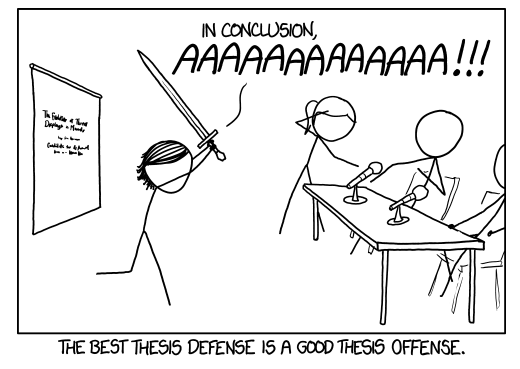
\includegraphics[width = 4.5in]{5_Appendices/Appendix_B/Figures/Thesis_Defence.png}
		\caption{You must prepare to defend your thesis \cite{xkcdThesis}} 
		\label{fig:DEFENCE}
	\end{figure}
\clearpage


% %*******************************************************************************
% % 0.9.2 - INDEX
% %*******************************************************************************
% % Creates the index
% % Uncomment if an INDEX should be created

% \printindex


%*************************************************************************************************************
% 1.0 - END OF DOCUMENT
%*************************************************************************************************************
\end{document}
